\chapter{Results \& Discussion}
\section{Introduction}
In this section, the results of the model discussed in Chapter 4 will be presented. In doing so, these results will answer the research question and sub-questions that were formulated in Chapter 1. Since this Thesis attempts to provide qualitative insights into CPT in an ABM framework and is less focused on forecasting a specific case study, the discussion of the results will emphasize on insights into the inner mechanics of the model. With the insights in this model, recommendations can be made with regards to the effect of different policies on the households' DER adoption and utility death spiral. As will become clear from the discussion in the subsequent sections, different policies will have very diverging effects on the adoption rate of PV and battery technologies as well as the network charge evolution. Depending on the goal of policy makers, therefore, different policies can be recommended. In Section \ref{compar}, the different policies will be evaluated by comparing the adoption rates, cumulative capacity, configuration adoption and utility death spiral for each of these policies. Subsequently, in Section \ref{analysis}, some deeper insights in the model shall be provided by analyzing the sensitivity of certain important parameters in the model. These parameters include the loss aversion, residual load and battery subsidy. The effect of the network charge on the model dynamics will also be a point of discussion. In Section \ref{EUTcompar}, the results of the CPT shall be compared with the EUT to discuss the advantages and/or drawbacks of these decision making theories. This chapter will be concluded with Section \ref{future}, where the results will be discussed, concluded and put in the context of broader research and future work.
\newline \newline \noindent
The presented results all come from code implemented in the JuMP environment that is part of Julia 1.1.1 \cite{julia}. The optimization problems were solved using the Gurobi package \cite{julia2}. All plots were generated using the PyPlot extension in the Julia environment.
\section{Policy Comparison}
\label{compar}
The main goals of this Thesis is to determine how different policies influence the adoption of DERs on a residential level. This adoption is to be considered both on a macroscopic level (i.e. what the overall adoption trend is) as well on a more microscopic level (i.e., how the adoption varies between the different configurations discussed in Table \ref{tab:config}). In addition to the adoption of the different configurations, the extent of the utility death spiral (i.e., the evolution of the distribution tariff) will be examined. The policies under evaluation are annual net metering, annual capacity offtake, net billing and battery subsidies (combined with annual net metering). The specifications for each of these policies are:
\begin{itemize}
\item \textbf{Annual net metering}: The prosumer will be able to sell his electricity to the grid at the same rate that he purchased it at. With the intention of decreasing noise in the model as much as possible, the energy price is assumed to be constant at a rate of 0.06 \EUR{}/\textit{kWh} (see Section \ref{development}). The price at which the household will sell his excess electricity will, therefore, also be a constant value of 0.06 \EUR{}/\textit{kWh}. The distribution cost to the prosumer will be determined by means of the net volumetric demand $q_{net}$ and a fixed distribution tariff $dist_{net}$.
\item \textbf{Annual capacity offtake}: Contrary to the previous policy, the annual capacity offtake will charge prosumers according to the peak capacity he will draw from the grid. This peak demand is selected on an annual basis. To make the starting point comparable for both the distribution and capacity tariff, the DSO revenue is assumed to be constant and the same in both cases, since the infrastructure that needs maintenance is the same. Since the DSO revenue for the distribution tariff is calculated as:
\begin{equation} \label{vol}
    Rev = dist_{net}*\sum^{households}_{i=1} q_{net,i}
\end{equation}
		and for the capacity tariff as:
\begin{equation} \label{cap}
    Rev = dist_{cap}*\sum^{households}_{i=1} q_{peak,i}
\end{equation}
Equations \ref{vol} and \ref{cap} can be combined to calculate the capacity tariff:
\begin{equation}
    dist_{cap} = dist_{net}*\frac{\sum^{households}_{i=1} q_{net,i}}{\sum^{ households}_{i=1} q_{peak,i}}
\end{equation}
Which results in a value of 465 \EUR{}/$kWh$. Combining this value with the peak demand of the household $q_{cap}$, the distribution component of the electricity bill can be computed. With regards to the energy component, the prosumer will be compensated and charged equally for the electricity injected into and consumed from the grid. 
\item \textbf{Net billing}: For this policy, the household will get a lower compensation for the electricity he injects into the grid. The tariff that will be used for this policy is a constant value of 0.05 \EUR{}/\textit{kWh}. This difference in tariffs will cause the household to have more incentive to save consumed electricity rather than sell injected electricity onto the grid. This policy will be combined with the net volumetric distribution tariff (similar to that of the annual net metering policy). 
\item \textbf{Battery subsidy}: Contrary to the previously discussed incentives, this policy helps in reducing the investment cost of a DER rather than increasing its operational revenue. This is done in order to encourage the adoption of batteries combined with PV. Since battery adoption has not achieved widespread scalability yet (see Section \ref{Trends}), some subsidies are required to make the technology affordable. In accordance with a recent incentive proposed by the Flemish government, a subsidy of 250 \EUR{} for each \textit{kWh} of residential battery capacity adopted will be introduced into the system \cite{subsidy}. Note that this subsidy is combined with the annual net metering policy in this Thesis. This is done since annual net metering is the most common policy up until now. 
\end{itemize}
These different policies will be evaluated. This will be done by considering the overall adoption, the adoption of the different configurations and the evolution of the network charges to examine the extent of the utility death spiral. 
\subsection{Technology adoption}
\subsubsection{PV}
For the different policies, the overall adoption of PV  technology can be seen in Figure \ref{Figure:PVvolpolicies}. This adoption is given both as a fraction of the entire population and as total capacity adopted. Note that the population consists of 6000 households, 3000 of which have the possibility to adopt DERs, meaning that a 50\% adoption fraction is equivalent to full adoption. The adoption processes of the different policies all follow the S-shaped adoption process like Rogers' innovation theory dictates: the adoption kicks off with a slow adoption (by innovators), followed by a period of steady adoption (when the majority of all actors adopt), only to finish by a saturating adoption by the end of the process, when the laggards will be involved in the adoption process. 
\begin{figure}[h!]
\centering
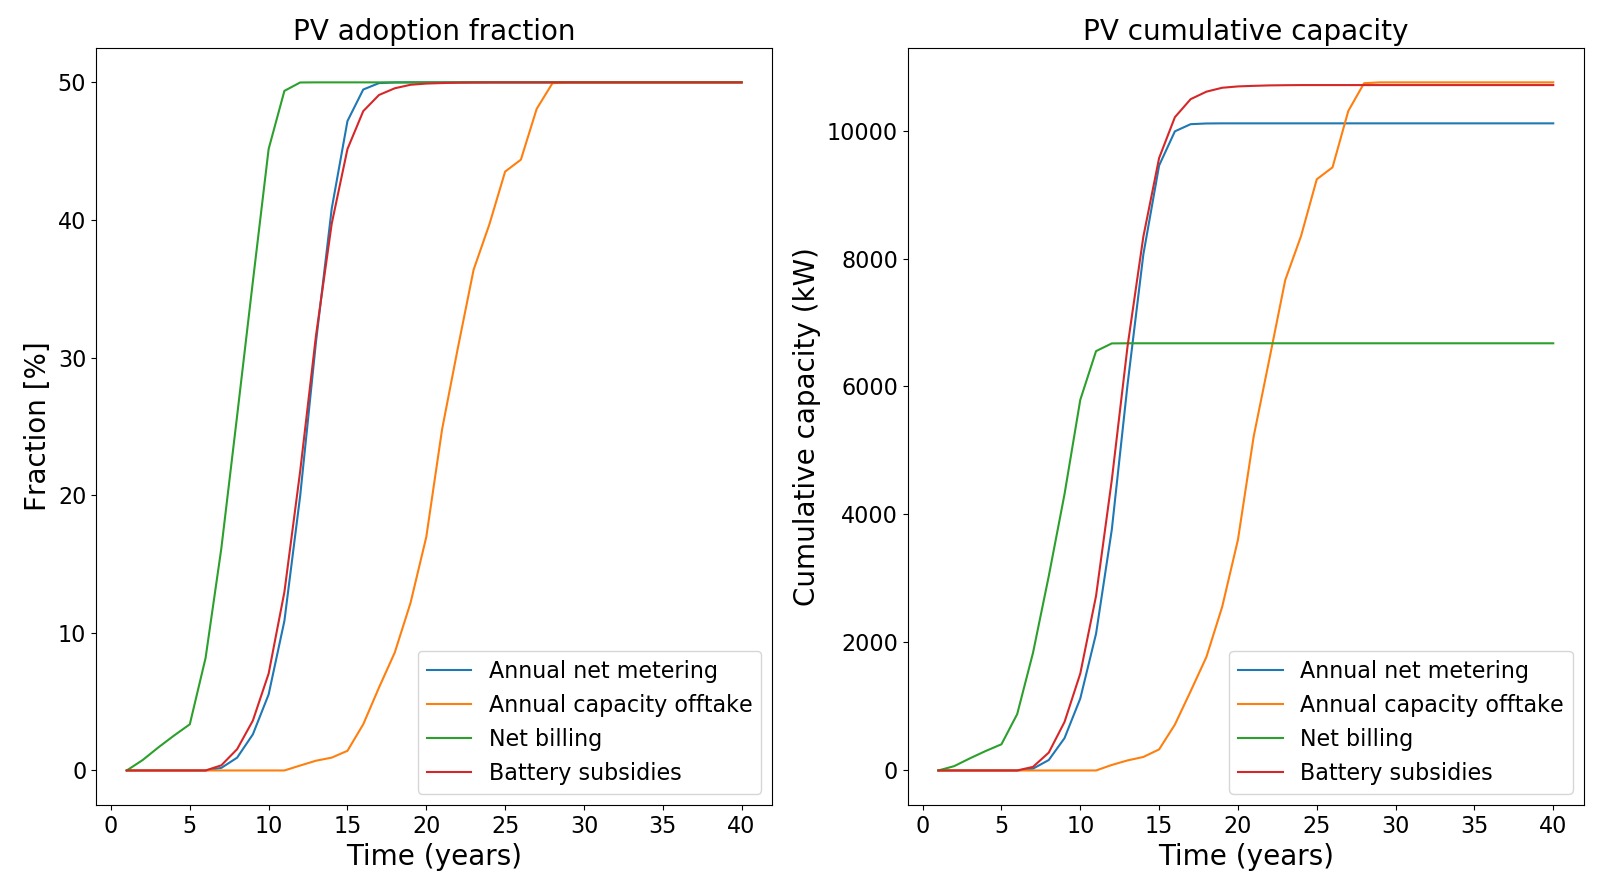
\includegraphics[width=12cm]{Policies/PV.png}
\caption{PV adoption for different policies}
\label{Figure:PVvolpolicies}
\end{figure}
\noindent
The PV adoption kicks off the latest for the capacity offtake tariff. The main reason for this later initiation of the adoption is the lower savings in the case of the capacity offtake tariff (see Section \ref{distanal}). Since the savings realised by the DER are lower, the households will have less incentive to invest. As time goes by, however, the configurations become cheaper. At a certain moment, therefore, the system cost will have sufficiently decreased to make the investment attractive despite the lower savings. Since the adoption in the capacity offtake case occurs almost 10 year later than in the volumetric tariff cases, the technologies are significantly cheaper. This will cause the larger configurations (and large PV panels in particular) to be the preferred option. This is why the overall capacity will be slightly higher for the annual capacity offtake case, even though full adoption is reached more than 15 years later than in the volumetric tariff cases. 
\newline \newline \noindent
The net billing policy will encourage households to become self-sufficient in their energy consumption by adopting DERs. The main reason for this trend in the adoption is the difference between the offtake and injection price of electricity. Since the households must pay 0.06 \EUR{} to consume a \textit{kWh} of electricity from the grid but receives only 0.05 \EUR{} for a \textit{kWh} of electricity injected into the grid, there is an opportunity cost for the household in injecting electricity into the grid. More money can be saved by avoiding electricity consumption than there can be made by injecting the same electricity into the grid. The selection of PV-battery installations will, therefore, mainly happen according to the optimal balance between the investment cost and the electricity savings the installation can bring about. This will make the households more prone to invest in the smaller installations that can supply most of their residential demand without injecting vast amounts of electricity into the grid. 
\newline \newline \noindent
The net metering policy, on the other hand, remunerates the households at the same rate for grid injection as it does for grid offtake. This makes it indifferent to the household whether their PV-battery installation avoids electricity consumption from the grid or whether the PV-battery installation consistently injects electricity into the grid. This will encourage households to install configurations that can maximize the benefits accordingly: the preferred configuration is one that avoids residential consumption while also injecting electricity into the grid. Larger configuration will be more suitable to fulfill this purpose. This will cause the overall adoption PV capacity to be larger for the net metering policy. Since these configurations will be more expensive, their adoption threshold will only be reached after 5 to 6 years, causing the adoption to kick off later for the annual net metering policy compared to net billing.
\newline \newline \noindent
By adding battery subsidies to the net metering policy, the PV adoption shows a similar trend. Although these subsidies do not directly affect the cost of the PV panels, the reduced cost of the batteries will cause the combined cost of several configurations to decrease, thereby making them more attractive to investors. Indirectly, therefore, the battery subsidies will make the PV technology more popular. Note that the overall adopted PV capacity in the case of the battery subsidies will be higher than for the net metering case without battery subsidies (about 5.9\%). At the same time, the adoption fraction for both annual net metering with or without battery subsidies is the same. This is because the battery subsidies will indirectly make larger PV panels in particular more popular. Since larger residential batteries tend to be installed together with larger PV panels (like the 4\textit{kW}/5\textit{kWh}), these configurations will become relatively much cheaper due to the subsidies. This will make the larger PV panels more popular among adopters, causing the average adopted PV size to increase, which results in a higher cumulative PV capacity for the battery subsidy policy. 
\newline \newline \noindent
%\noindent
%\begin{table}[h]
%\centering
 %\begin{tabular}{||c|c|c|C||} 
 %\hline
 %\textbf{Policy} & \textbf{Adopters} & \textbf{Capacity (\textit{kW})} & \textbf{PV
 %/Adopter (\textit{kW})}\\
 %\hline \hline
 %Annual net metering & 3000 & 10,112 & 3.37 \\
 %Annual capacity offtake &3000 & 10,752 & 3.58\\
 %Net billing & 3000 & 6,675 & 2.23\\
% Battery subsidies & 3000 & 10,710 & 3.57\\
% \hline
% \end{tabular}
% \caption[Overview PV adoption data]{Overview PV adoption data}
% \label{table:threshold}
%\end{table}
%\noindent
Due to the difference in incentives between the different policies, the adoption patterns will be different. The annual offtake policy will cause a late kick-off in the adoption but due to the decreased costs, full adoption is reached (i.e. 3000 households) and the cumulative PV capacity even surpasses that of the volumetric tariffs, at a value of 10,752\textit{kW} . This results in a PV capacity of 3.58\textit{kW} per household. Since the smaller, less expensive configurations will be more popular in the net billing case, the adoption threshold for these configurations will be reached quite early in the simulation (year 2-3). The adopted capacity, however, will converge to a value of  6675\textit{kW}. This means that the average adopted PV capacity (among the 3000 households) is 2.23\textit{kW}. Given the fact that the possible PV sizes are 1.5, 2.5 and 4\textit{kW}, the majority of the adopted PV panels will be of the 1.5\textit{kW} kind. For the net metering case, full adoption will also be reached, but this process will be slightly delayed compared to the net billing policy, since the preferred configurations (that can inject significantly into the grid) will only reach the adoption threshold later on in the simulation, mainly due to the cost reduction effects. Compared to the net billing policy, however, the overall adopted capacity will be higher. The final adopted capacity is 10,112 \textit{kW}. Given the fact that 3000 households will adopt PV panels, the average PV capacity installed is 3.37\textit{kW}. Since possible PV configurations are 1.5, 2.5 and 4\textit{kW}, a large amount of 4\textit{kW} panels will be adopted in the annual net metering policy. When subsidies are added to the net metering policy, the aggregate capacity increases to 10,710\textit{kW}. Since the adoption fraction also is 50\% in this policy, 3000 households will adopt PV panels, bringing the average per household to 3.57\textit{kW}. The average PV capacity per household will, therefore, be 5.9\% higher with battery subsidies. A summary of these results can be found in Figure \ref{Figure:pvav}. 
\begin{figure}[h!]
\centering
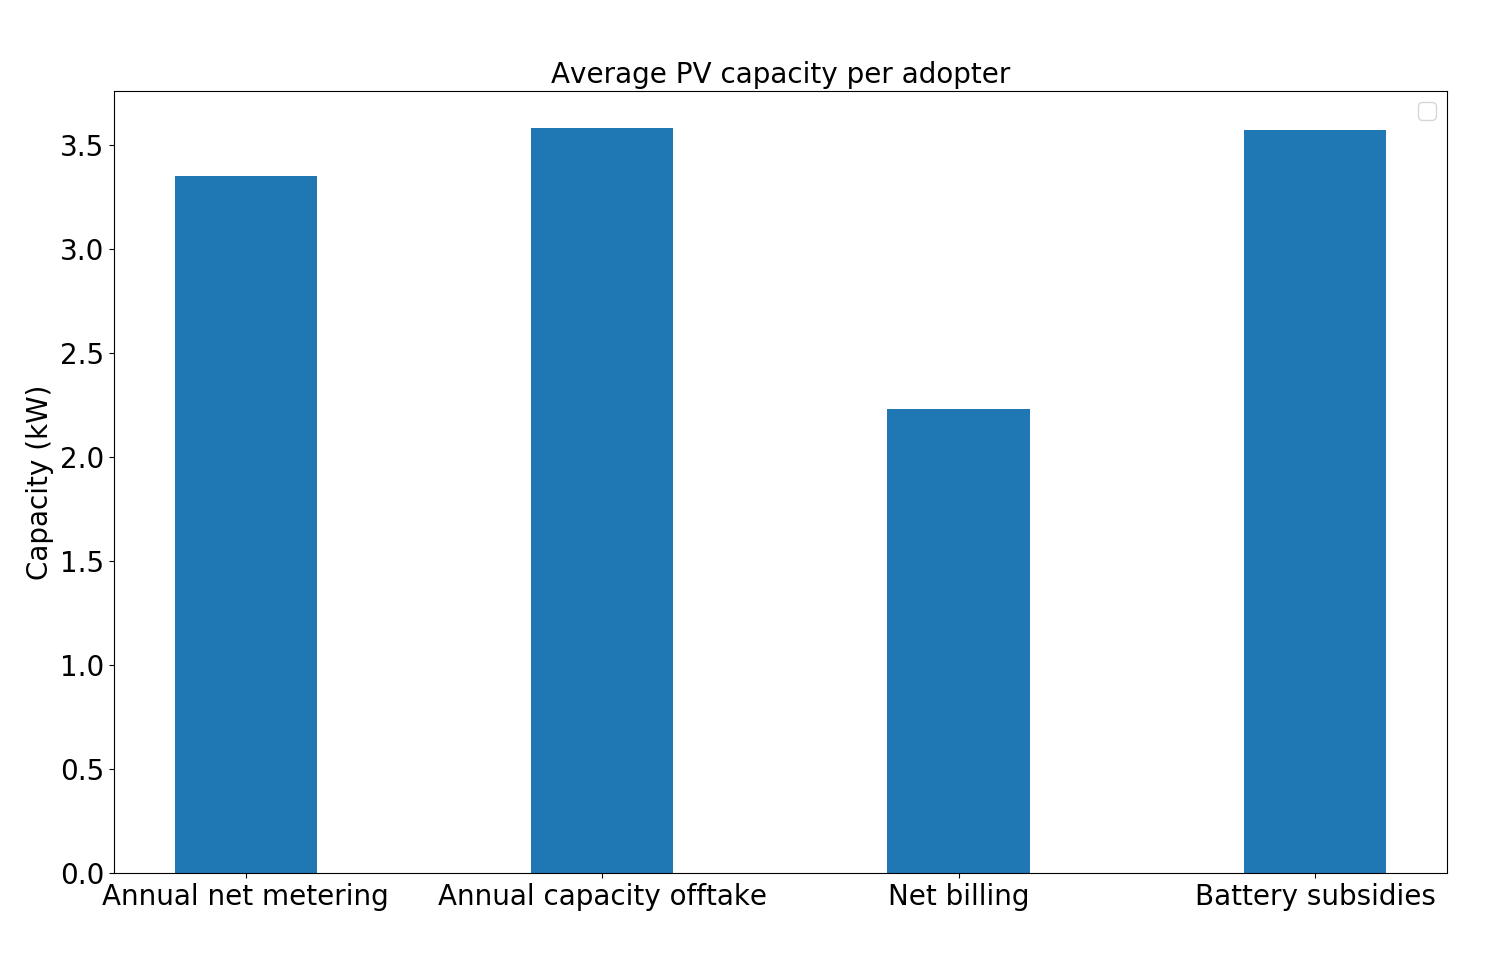
\includegraphics[width=10cm]{Policies/AvPV.png}
\caption{Average PV capacity per household}
\label{Figure:pvav}
\end{figure}
\subsubsection{Batteries}
The battery adoption evolution can be found in Figure \ref{Figure:batpolvol}. The adoption of this technology also follows the S-shaped curve dictated by Rogers' Innovation Theory. Contrary to the PV adoption data, the battery technology adoption is relatively low for the annual capacity offtake tariff. This is due to the difference in costs between PV and batteries: PV panels are a cost competitive technology but batteries still are in heavy development. The latter technology remains expensive compared to the former: note how PV subsidies no longer exist but battery subsidies are a recent government incentive to encourage adoption of this technology \cite{subsidy,Zonnepanelen}. Since the households will realize lower savings under the annual capacity offtake policy, there will be less incentive to invest in expensive batteries. This will cause the cumulative battery adoption capacity to be relatively low compared to the PV adoption levels of the policy.
\newline \newline \noindent
As was the case with the PV adoption data, the battery adoption capacity is relatively low for the net billing case. The battery adoption fraction, however, is also very low compared to the other policies. This is because the preferred configurations are those that save the household the most money due to avoided electricity consumption rather than vast grid injections at minimal investment cost. Since this will cause the total savings the household can realize to be lower, the smaller configurations (i.e. standalone PV panels or panels with a 2\textit{kWh} battery) will be the most popular candidates to fulfill this requirement. Due to these lower savings, the expensive batteries will be less popular among adopters, causing the overall adoption fraction and capacity to be lower. Since the cheaper configurations are the preferred ones, the adoption threshold for these configurations will be reached very early on in the model, causing the net billing adoption process to start the quickest for battery technologies.
\begin{figure}[h!]
\centering
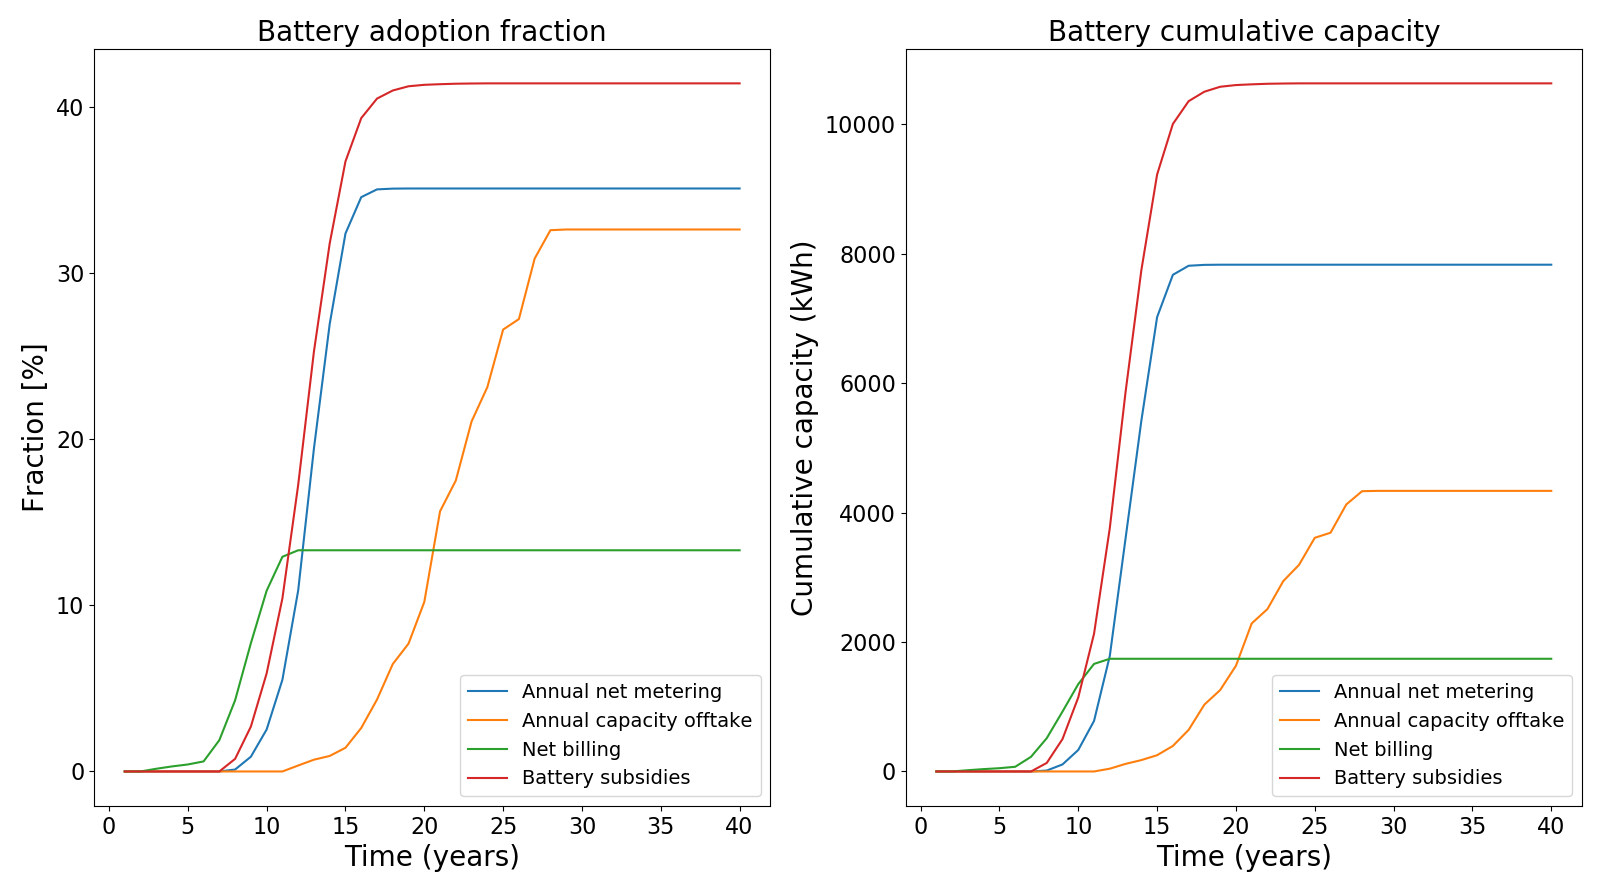
\includegraphics[width=12cm]{Policies/Battery.png}
\caption{Battery adoption for different policies}
\label{Figure:batpolvol}
\end{figure} 
\noindent
For the net metering case, on the other hand, the battery adoption fraction and capacity adopted will be higher than in the net billing case. This is mainly because net metering encourages households to adopt DER for both avoiding grid offtake and increasing grid injection. Larger configurations, therefore, can serve as a means to increase the revenue from continuous grid injection. 
\newline \newline \noindent
The effect of the battery subsidies on the adoption levels is visibly positive. Compared to the net metering case, upon which policy these subsidies are added, the battery subsidy policy shows cumulative adoption capacities that are 35.7\% higher than the case without batteries. Note that the adoption process in the case of the battery subsidies will also happen slightly faster than the case without any financial aid. Battery subsidies will, therefore, incentivize a slightly smaller number of households to adopt larger, more expensive technologies. To accelerate the adoption of large batteries, the battery subsidies can help significantly. When looking into the data of the different policies, the effect of the different policies on the technology adoption becomes even more clear. Since the adoption rate for the annual capacity offtake policy is 32.6\% (i.e. 1956 households) for a cumulative capacity of 4337\textit{kWh}, the average battery capacity per adopter under this policy will be 2.22\textit{kWh}. Since the available options for the batteries are either a 2\textit{kWh} or 5\textit{kWh} module, the average capacity per adopter suggest that the overwhelming majority of adopters will opt for the 2\textit{kWh} alternative.	Since the net billing policy will inherently favor smaller configurations, the average battery capacity per adopter also is smaller: 2.18\textit{kWh}. This is the result of a 13.3\% adoption fraction (which accounts for 798 households) for a cumulative capacity of 1742\textit{kWh}. The annual net metering policy, on the other hand, will make the households prefer larger configurations to increase the benefits of grid injection. Since the adoption fraction is 35.1\% (i.e., 2100 households) and the cumulative capacity is 7832\textit{kWh}, the average battery capacity for each adopter will be 3.73\textit{kWh}, which is significantly higher than the other cases. When considering the available options (2\textit{kWh} \& 5\textit{kWh}), it becomes clear that the average adoption trend has clearly shifted towards the larger alternative. Introducing battery subsidies on top of the annual net metering will cause the overall capacity to increase by 24.7\% to 10,635\textit{kWh} while the adoption fraction will increase from 35.1\% to 41.4\% (2484 households), causing the average battery capacity per adopter to increase by 14.7\% to 4.28\textit{kWh}. This clearly shows how the battery adoption trend will be shifted even more to the larger configurations when battery subsidies are added. A summary of this data can be found in Figure \ref{Figure:batav}.
\begin{figure}[h!]
\centering
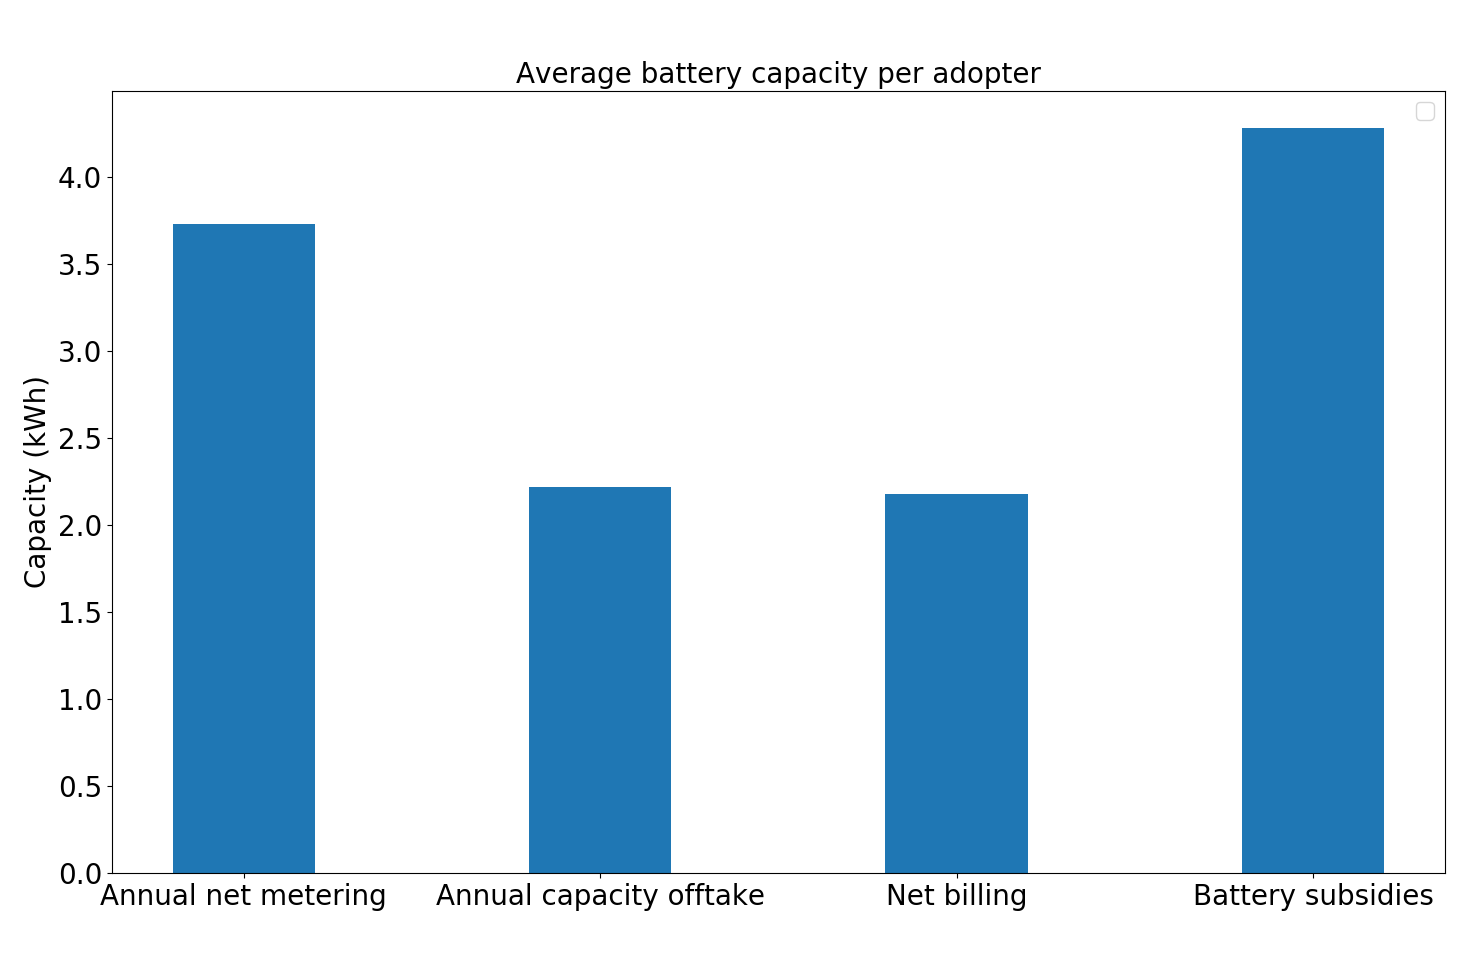
\includegraphics[width=10cm]{Policies/AvBat.png}
\caption{Average battery capacity per household}
\label{Figure:batav}
\end{figure}
\subsection{Configurations}
Besides examining the overall adoption trend, a look into the adoption of the different configurations is also a useful insight into the evaluation of different policies. Figure \ref{Figure:configpol} shows how the different policies drive the popularity of different configurations. Both annual net metering and the same policy combined with battery subsidies favor the larger, more expensive configurations since grid injection can bring substantial benefits to the prosumer. The annual capacity offtake and net billing policy, on the other hand, will make the small and medium-sized configurations more popular. Since the injection tariff is lower than the offtake tariff for the net billing case, self consumption is encouraged and grid injection is discouraged, causing the smaller/less expensive configurations to become more popular.  For the annual capacity offtake case, the combined effects of lower savings and cheaper configurations due to delayed adoption will make the smaller medium-sized installations slightly more popular, with a focus on the larger standalone PV panels (2.5\textit{kW} and 4\textit{kW}) and larger PV panels with a smaller battery (2.5\textit{kW}/2\textit{kWh} and 4\textit{kW}/2\textit{kWh}).  
\begin{figure}[h!]
\centering
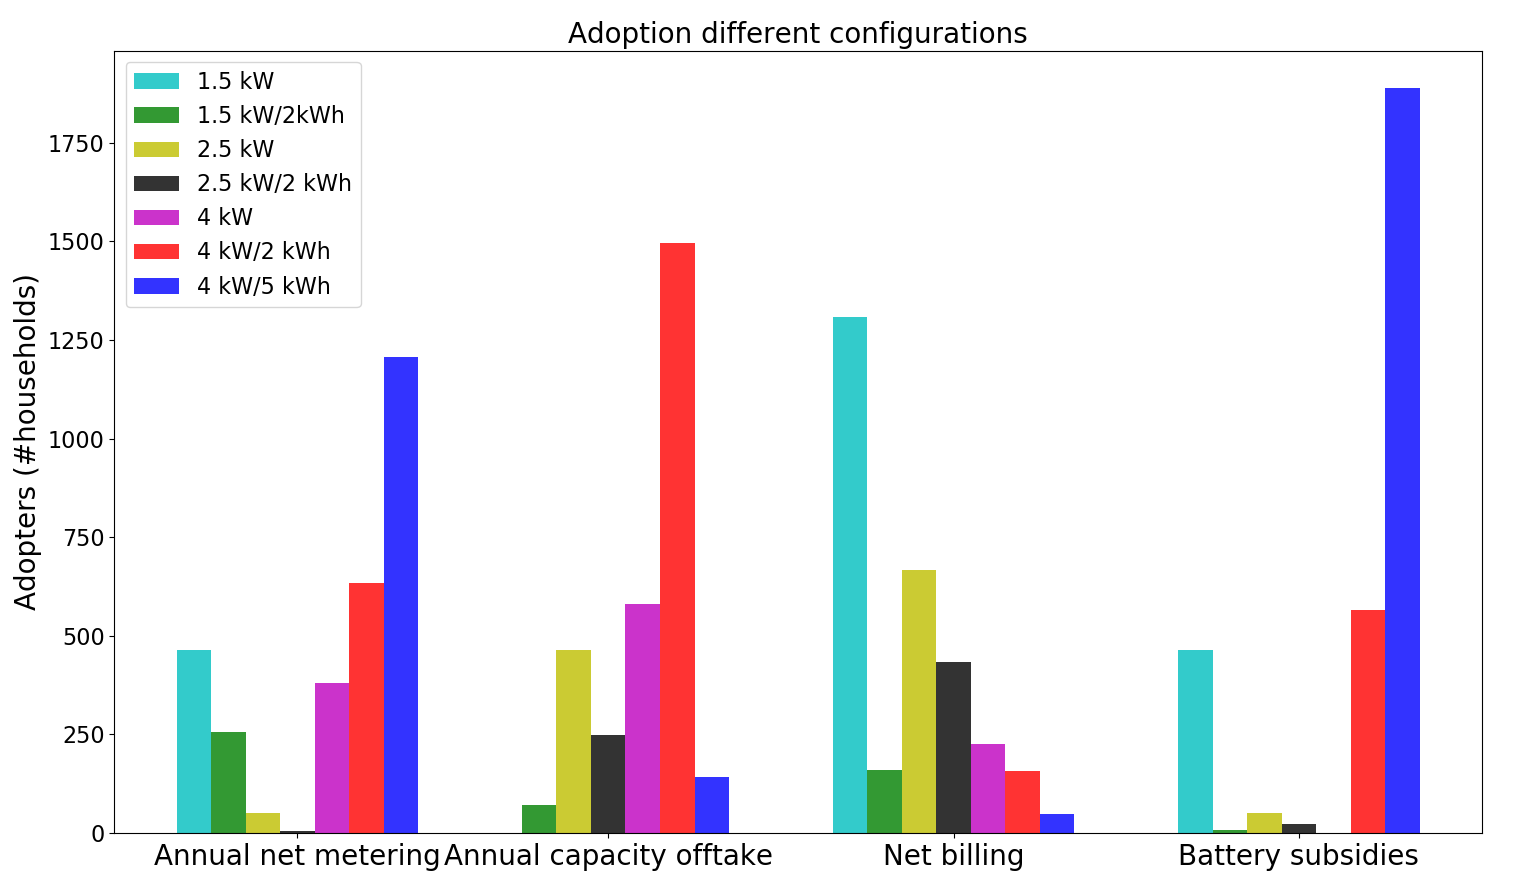
\includegraphics[width=12cm]{Policies/Configurations.png}
\caption{Configurations adoption for different policies}
\label{Figure:configpol}
\end{figure}
\noindent
This adoption data, combined with the adoption processes discussed in the previous section, already gives some insights into the value of different policies to encourage DERs adoption. Policy makers, therefore, should consider these different policies depending to their priorities. 
\newline \newline \noindent
If the goal of the policy makers is to make households adopt PV panels with an optional battery to fulfill their own residential demand, the net billing policy is the most effective. The pricing strategy implied in this renewables scheme will make households adopt PV-battery systems that provide sufficient electricity to supply the majority of the residential demand of the prosumer. The households will be less motivated by the possibility to export excess electricity into the grid. This policy, therefore, implicitly mitigates the widespread injection of residential PVs into the grid, thereby avoiding many grid stability issues.
\newline \newline \noindent
Besides limiting the utility death spiral (see next section), the annual capacity offtake tariff can also help in making the adoption of the different configurations more distributed across the small and medium-sized configurations, with a slight bias toward the standalone 4\textit{kW} and 4\textit{kW}/2\textit{kWh} configuration. The combination of slightly lower savings that the household will be able to realize and the cheaper configurations due to delayed adoption will give him less incentive to adopt the largest configurations (as the net metering and battery subsidy policy do). If policy makers want to change the network charge in the grid while at the same time ensuring a reasonably distributed adoption of different adoptions, the annual capacity offtake policy is a promising candidate. 
\newline \newline \noindent
If, on the other hand, policy makers want to encourage a widespread adoption of larger DER configurations on a residential level to increase the overall produced energy, net metering is the preferred policy. This policy will encourage households to adopt both to supply their residential demand and sell excess electricity to the grid. Although this policy increases the overall adopted DERs capacity and the energy produced by them, it can also bring about grid stability issues. If policy makers want to amplify this effect, battery subsidies can be added to the mix to encourage further adoption of large batteries. 
\subsection{Utility death spiral}
Due to the adoption of the DER on a residential level, the aggregate energy demand of the households will gradually decrease. This will cause the DSO revenue to come under threat, which could make it difficult for the grid operator to maintain and upgrade his infrastructure. As a reaction, the DSO will adapt his pricing towards the end customers. In the case of the annual capacity offtake tariff, the DSO will also need to adapt its pricing since the DER adoption will cause the aggregate peak demand taken from the grid to decrease (a further discussion of these interactions in the model can be found in Section \ref{distanal}). Since the evolution of two different network charges is to be evaluated, the normalised values will be compared. The evolution of these normalised values for the different policies can be seen in Figure \ref{Figure:distpol}. 
\begin{figure}[h!]
\centering
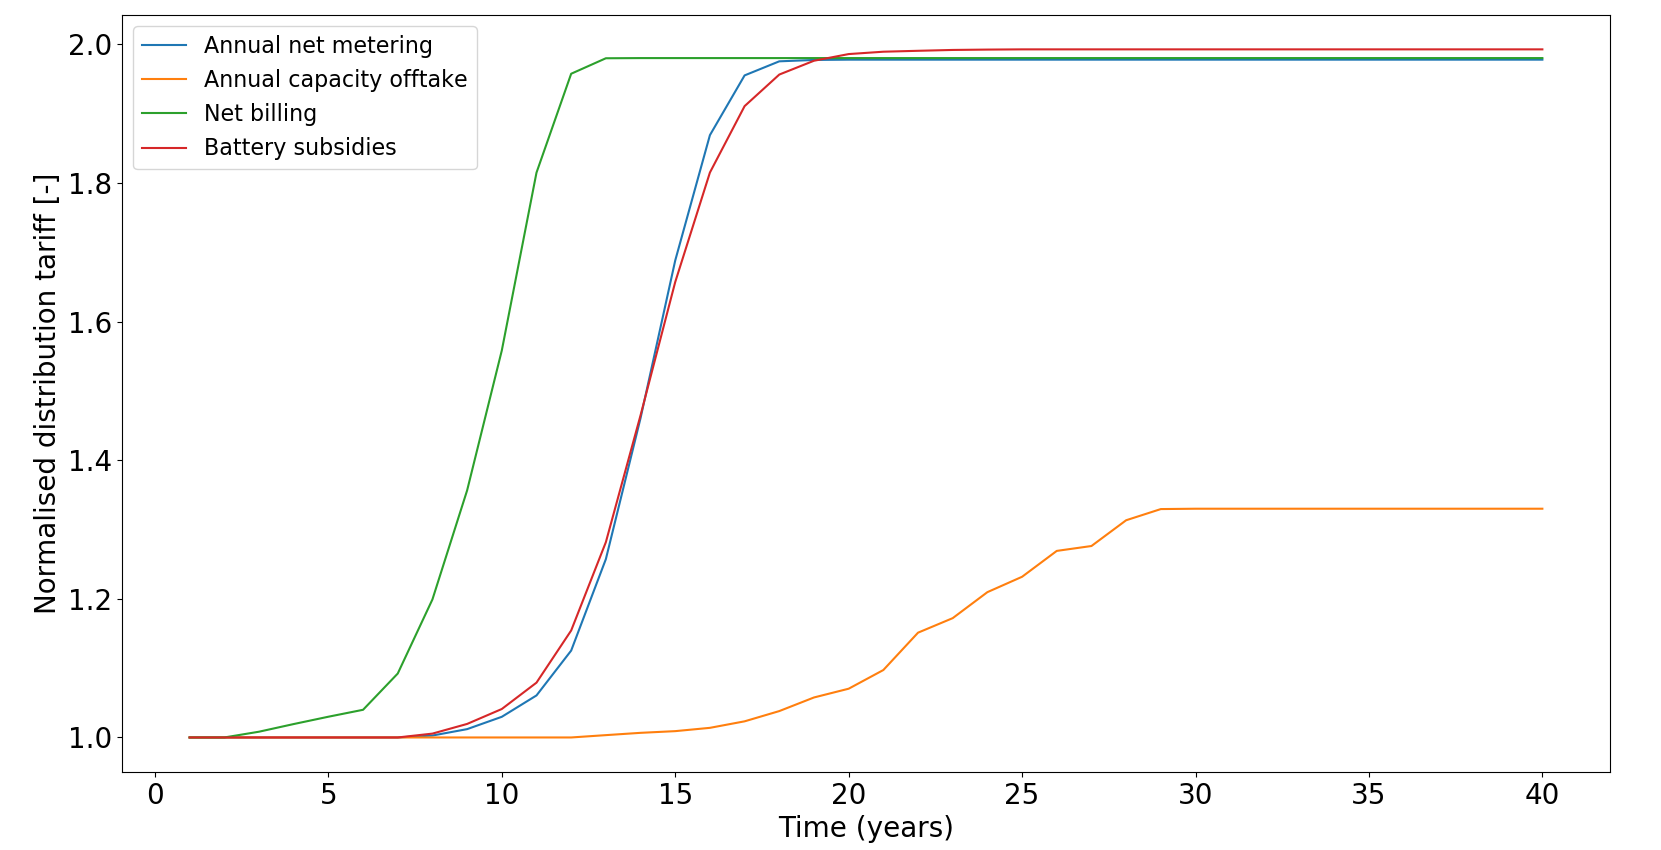
\includegraphics[width=6cm]{Policies/Dist.png}
\caption{Normalized distribution tariff evolution for different policies}
\label{Figure:distpol}
\end{figure}
\noindent
The evolution of the distribution tariff shows a trend that runs in parallel with the DERs adoption: for the quick adoption of the net billing policy, the distribution tariff increases more quickly than for the annual net metering and supplementary battery subsidies case, where DER adoption occurs less quickly. The contrast of the evolution for the volumetric tariff policies with the capacity tariff, however, is the most important trend that can be spotted in this figure. Whereas the distribution tariff increases by  97.8\% in the case of the annual net metering, 98.0\% in the case of net billing and 99.3\% for the battery subsidies case, this increase will only be by 33.0\% in the capacity offtake case. This is a significant difference in tariff evolution. Considering the PV adoption levels for the annual capacity offtake policy, which exceed those of all volumteric tariff-based policies, this limited increase in network charge shows the potential benefits of the annual capacity offtake tariff. 
\newline \newline \noindent
The utility death spiral is, therefore, a phenomenon that will clearly demonstrate itself when a DSO is faced with large DER adoption rates among his customers. Whereas this vicious process will be very clear in the volumetric distribution tariff policies, the capacity offtake tariff will be able to mitigate this effect significantly. 
\subsection{Preliminary analysis \& Conclusion}
The data presented in this section shows how the DER adoption and utility death spiral manifest themselves for different energy-related policies. These results can already lead to certain preliminary conclusions, comparisons and reflections. These will be the main point of discussion for the remainder of this section. 
\newline \newline \noindent
Since the most common policy concerning residential PV is annual net metering, the presented results challenge this choice of policy. Other policies like net billing and the annual capacity offtake show a very different adoption and network charge profile. Among these different alternatives, the efficiency of each one can be evaluated. An adequate DER policy enhances the adoption of these technologies while minimizing the effects/damage to actors other than the households involved or implicated in the adoption process. The most important actor in this aspect is the DSO\footnote{There are many additional actors in this process like the TSO and BSP, but to keep the discussion straightforward, the DSO is a "representation" of the different grid actors}. The important aspects to judge a policy are:
\begin{itemize}
    \item \textbf{Adoption:} The main objective of a DER policy is the diffusion and widespread adoption of PV and battery technology. This adoption should happen quickly (i.e., within an acceptable period of time) and should result in sufficient generation capacity to provide the majority of the residential household electricity demand. 
    \item \textbf{Utility death spiral}: The adoption of the DER should not cause the revenues of the DSO to drop dramatically, since this would make it challenging for the latter to maintain and upgrade his infrastructure, forcing him to adapt the network charges, creating a vicious process that is the utility death spiral. This factor should also be accounted for in the policy choice. 
    \item \textbf{Grid injection \& other}: Although this Thesis mainly focuses on the two aforementioned evaluation parameters, grid injection and the subsequent grid stability issues should also be selection criteria for a policy. Since continuous grid injection by residential DER makes the grid less stable and reliable unless additional reserve and storage capacity is provided, a great deal of costs and headached on behald of the grid operator can be avoided by putting a policy into action that encourages households to adopt DER that limits the amount of grid injection. In the context of this Thesis, the policy must make the households on average prefer smaller configurations over larger configurations.
\end{itemize}
When considering all the available policies (and all possible permutations that could be composed), a few things become clear. The current policy, being annual net metering, scores relatively poorly when considering the evaluation parameters. Although this policy will cause the cumulative adopted DER capacity and subsequent renewable energy produced to be substantial, the adoption process that leads up to this capacity will be relatively slow. For the first evaluation parameter, therefore, the annual net metering will score reasonably well. The next two parameters, however, will perform poorly under this policy: judging by Figure \ref{Figure:distpol}, the utility death spiral effects will be substantial. Since the average adopted DER capacity is large, the grid injection will also be significant. For both criteria, better alternatives have emerged from the results. With regards to the utility death spiral, the annual capacity offtake certainly is the favored candidate (see Figure \ref{Figure:distpol}). By introducing a capacity-based network charge, this vicious circle of DER adoption can be partially avoided. This policy does, however, show the slowest adoption for both PV and battery configurations. The adoption for this policy kicks off ten years later compared to net billing. Judging by Figures \ref{Figure:batpolvol} and \ref{Figure:batav}, the net billing policy will cause the adoption to occur more rapidly. Since the average adopted DER capacity also is lower for this policy, the grid injection will be lower. 
\newline \newline \noindent
The presented results do bear some similarities with previous work in this domain. Previous work attempted to simulate the PV adoption using the EUT. In doing so, many different utility attributes were used, such as advertisement, income and environmental factors \cite{ABMPV,ItalyAdoption}. The adoption results of these studies will be compared to the model developed in this Thesis. The results of the PV adoption by Palmer et al. can be found in Figure \ref{Figure:italyadoption}: 

\begin{figure}[!tbp]
  \centering
  \begin{minipage}[b]{0.4\textwidth}
    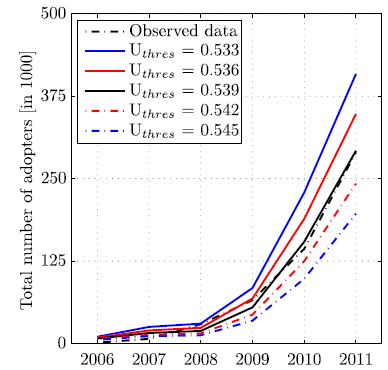
\includegraphics[width=6cm]{Policies/Italyadoption.PNG}
    \caption[PV adoption data Palmer et al.]{PV adoption data Palmer et al. \cite{ItalyAdoption}}
    \label{Figure:italyadoption}
  \end{minipage}
  \hfill
  \begin{minipage}[b]{0.4\textwidth}
    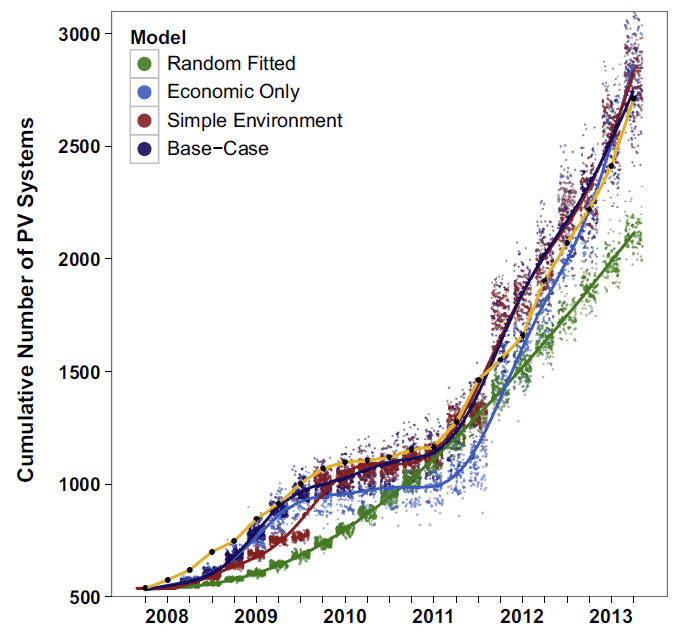
\includegraphics[width=6cm]{Policies/robinsonadoption.PNG}
    \caption[PV adoption data Robinson and Vai]{PV adoption data Robinson and Vai \cite{spatiotemp}}
    \label{Figure:spatiotemp}
  \end{minipage}
\end{figure}
\noindent
In addition, the adoption data obtained by Robinson and Vai can be found in Figure \ref{Figure:spatiotemp}. When comparing this data to the adoption data of this Thesis, as can be seen in Figure \ref{Figure:adopters}, there is a clear similarity with all policies, with the exception of the annual capacity offtake program. All other policies show how the PV adoption kicks off at initially slow rates, followed by a ramp-up in the adoption (which represents an exponential adoption trend). Note how the annual net metering and battery subsidies show the biggest similarity. This data is a good illustration of how new technologies like PV and batteries will emerge. 
\noindent
Note that the time between no adoption and the exponential adoption take between four and five years for both works: For Palmer et al., the adoption starts in 2006 and ramps up exponentially until 2011, while for Robinson and Vai the adoption starts in 2008 and ramps up exponentially until 2013. The data in Figure \ref{Figure:PVcompar} shows a similar trend: for both the annual net metering and battery subsidies, the adoption kicks off in year 6 and has become an exponential by year 10. For the net billing, the adoption kicks off in year 4 and also becomes exponential by year 10. 
\begin{figure}[h!]
\centering
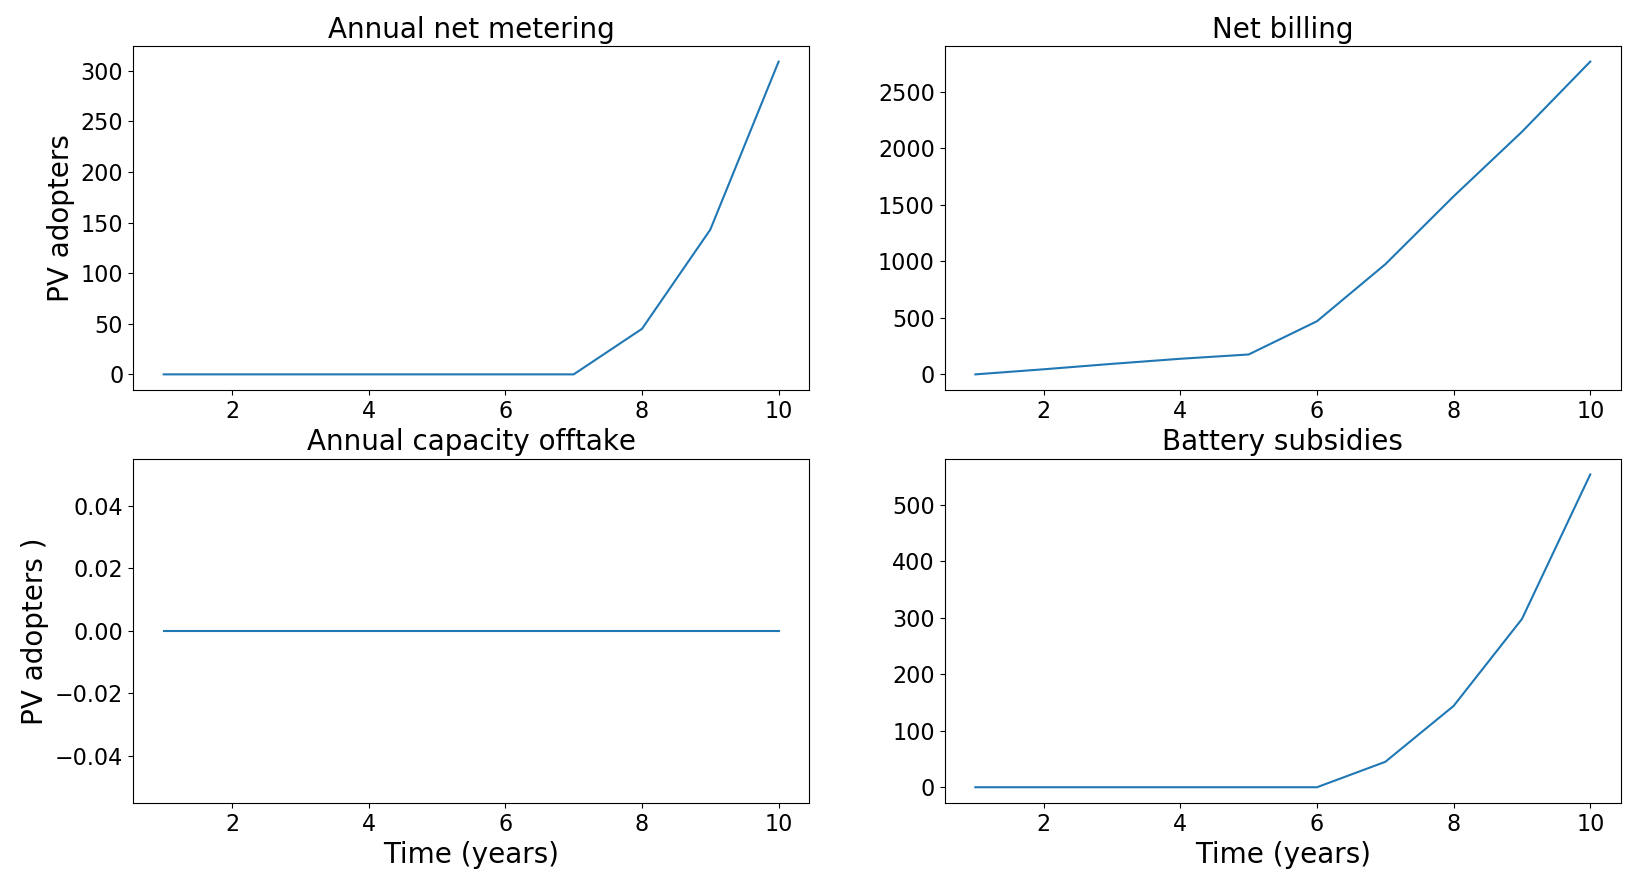
\includegraphics[width=12cm]{Policies/AdoptersCompar.png}
\caption{First ten periods adoption data different polices}
\label{Figure:adopters}
\end{figure}
\noindent
When comparing the data tot that of Zhao et al., as can be seen in Figure \ref{Figure:zhao}, the adoption is considered over a longer period.
%\begin{figure}[h!]
%\centering
%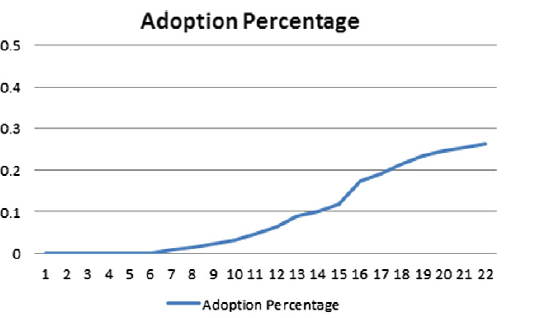
\includegraphics[width=6cm]{Policies/Zhao.PNG}
%\caption[PV adoption Zhao et al.]{PV adoption Zhao et al.  \cite{ABMPV}}
%\label{Figure:zhao}
%\end{figure}
%\noindent
The adoption shows an S-shaped profile, as Rogers' Innovation Theory dictates. This adoption process takes 16 years. When comparing this to the overall adoption data in Figure \ref{Figure:PVvolpolicies}, the PV adoption for the case of net metering starts in year 6 and converges to its final adoption fraction in year 18. The adoption period, therefore, takes 12 years, which slightly lower compared to the adoption period determined by Zhao et al.. Both for the start of the adoption and the entire adoption period, therefore, the results from this Thesis bear many similarities with related works. 
\newline \newline \noindent
The data obtained in this Thesis does, however, show a slightly more uniform trend than the results of the related works. This is due to the lower amount of households considered in this Thesis (3000 vs. 100,000s in other works), causing the heterogeneity of the system to be smaller. This will inevitably cause less values to deviate from the general trend. Since the utility attributes in this Thesis are limited to the welfare and peer effect (since the main purpose was to examine the effects of using CPT in the DER adoption process), the results will behave according to these attributes. The more of these attributes are added, the more complex the behavior of the results will be. Nevertheless, the overall trend of the data obtained in this Thesis is very similar to the one presented in the works by Palmer et al., Robinson and Vai and Zhao et al.. As was discussed in Chapter 3, CPT still faces many challenges before being accepted as an operationalizable model. The main challenge is a general convention for the values of the loss and risk aversion as well as an adequate selection of the reference level to the decision maker. These values, therefore, had to be estimated using both common sense and trial and error in the simulations, since there is no literature available to select generally accepted values. Despite this approach, the results of the model make a lot of sense when comparing them to the Innovation Theory developed by Rogers and the results of other works in this domain of science. 
\newline \newline \noindent
Despite these findings, the results of the model should be treated with a level of scrutiny. Since the utility in this model only considers the welfare and peer effect utility to a certain decision, several aspects of decision making are not accounted for. If the households also incorporate environmental, communication or advertisement effects into their decision making, the decisions influenced by these factors cannot be captured by this model. In addition, the weighting coefficients of Equation \ref{eq:ut} are assumed to be constant throughout the simulation. This gives a level of staticity to the model, despite the intention of this model being to capture the dynamics of the DER adoption process. In next stage, the weighting coefficients should be made endogenous to the model. The author of this Thesis shares this concern with Palmer et al. \cite{ItalyAdoption}. In this work, the authors opted for constant weighting coefficients since they found no mechanism to include this coefficient change into the model. In the setting of this Thesis, however, some recommendation for this change in coefficients can be made. Since the adoption will initially be driven by economic incentives, the economic coefficients should be higher in the beginning of the model. Subsequently, as the adoption increases and the peer effect starts to manifest itself, the economic weighting coefficient of the utility decreases. In parallel, the social weighting coefficient increases. The exact values of this increase and decrease are difficult to postulate and have to be determined by careful analysis and comparison of the model results with actual adoption data. 
\newline \newline \noindent
Another limitation of the model is the strict segregation between the different policies, with the exception of the battery subsidies. From the results discussion, it became clear that every policy has its specific characteristics, like the quick adoption for net billing or higher average capacity for net metering. In reality, however, the potential solution will be a combination of all available options. In a further stage, therefore, different combinations of the policies must be tested to determine the optimal policy combination. 
\section{Model Analysis} \label{analysis}
Given the overall adoption trends, some elements need further discussion. A few key parameters embedded in the model require further analysis. To understand their role in the model, a sensitivity analysis will be performed of these parameters. This sensitivity analysis will be performed for the loss aversion and battery subsidies\footnote{Since the author was constrained by the size of this Thesis, the discussion of the residual load and network charge could not be included in the report but can be found on: }.
\subsection{Loss aversion}
Since this Thesis uses a novel approach of CPT in an ABM to simulate the adoption of DERs, a deeper study into the sensitivity of the parameters governing the prospect value computation is to be performed. The most important variable in prospect theory, besides the prospect value, is the loss aversion parameter $\lambda$. This parameter will indicate how strong the convexity of the loss-facing part of the value function will be (see Figure \ref{Figure:value}). The higher the loss aversion coefficient, therefore, the more negative the prospect value of a negative prospect will be, making the decision maker more willing to take risks to make up for his losses. The inverse is true for a lower value of the loss aversion coefficient. To test this consistency of the model, different values for the loss aversion will be tested to see what effect this has on the model output. Since the value used in this Thesis is $\lambda = 1.5$, variations on this base case can be tested and compared with each other. A first interesting value would be a case where the loss aversion does not amplify the prospect value in the negative domain (i.e., $\lambda = 1$). The second value that will be tested is a loss aversion coefficient larger than the one in the base case, which will be chosen at $\lambda = 2$.  All simulations will be done with the same value for the risk aversion (i.e., $\alpha = \beta = 0.6$). This analysis will be discussed for the net metering policy in this section. The other policies can be found in Appendix \ref{app:2}. 
\newline \newline \noindent
The PV adoption results for the different loss aversion values can be found in Figure \ref{Figure:PVlossvol}: 
\begin{figure}[h!]
\centering
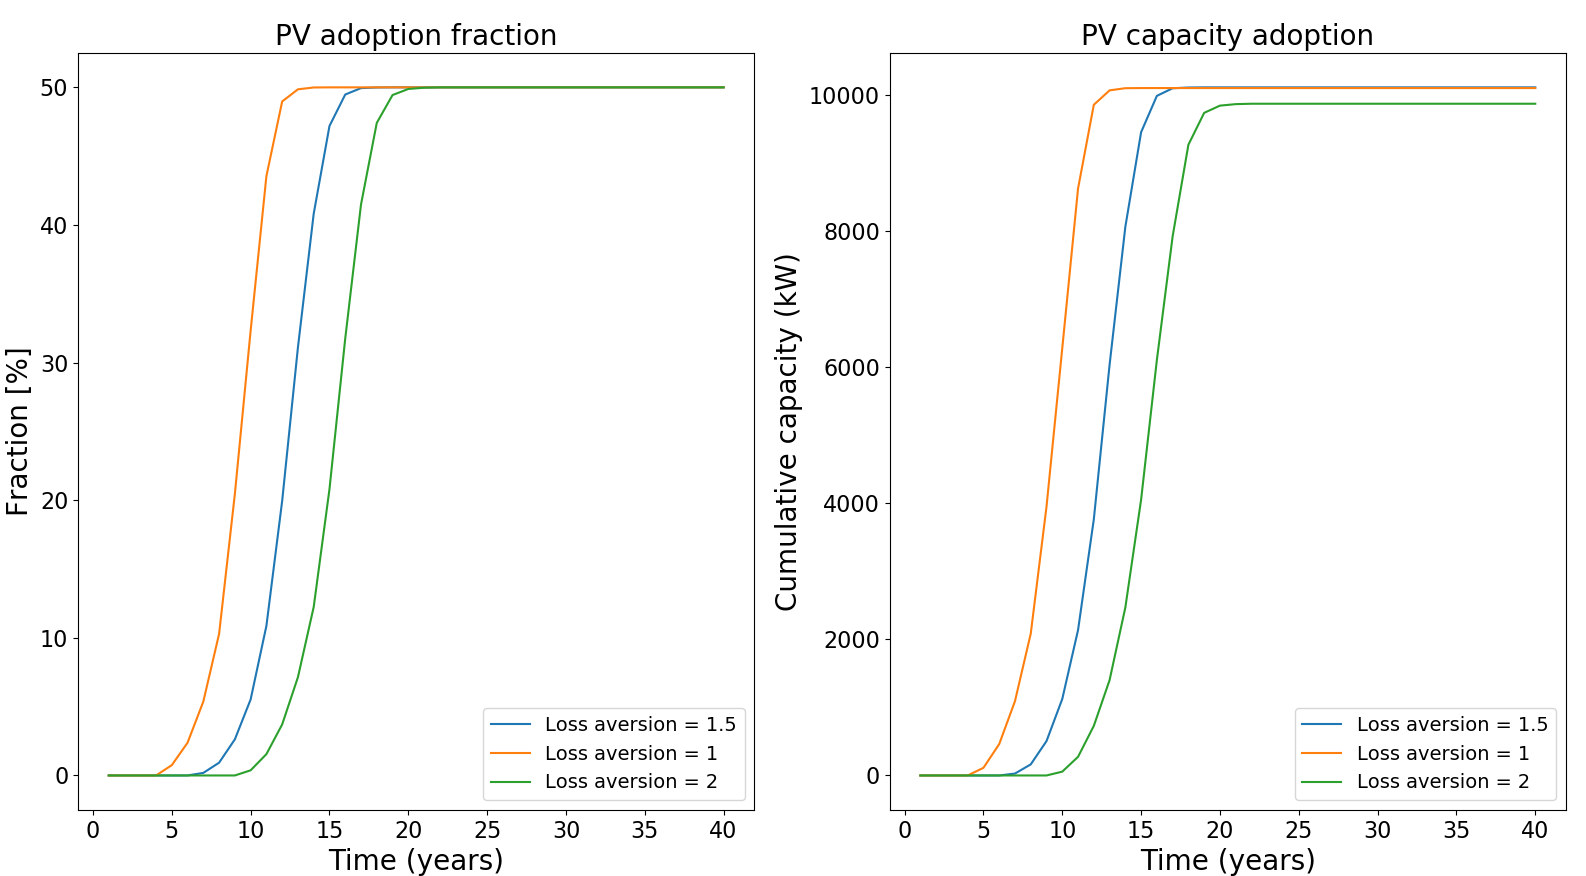
\includegraphics[width=12cm]{ModelAnalysis/PVloss.png}
\caption{PV adoption for different loss aversions}
\label{Figure:PVlossvol}
\end{figure}
\noindent
In this figure, the effect of the loss aversion on the output can be clearly seen: for lower loss aversions, the adoption happens more quickly: whereas in the normal simulation the adoption kicks of in year 7, this already happens in year 4 for the low loss aversion. For the higher loss aversion, the adoption starts later (year 10) and will converge to a slightly lower value. The adoption data for the high loss aversion will show a slightly lower PV capacity than the low loss aversion case. The battery adoption data can be found in Figure \ref{Figure:batlossvol}. 
\begin{figure}[h!]
\centering
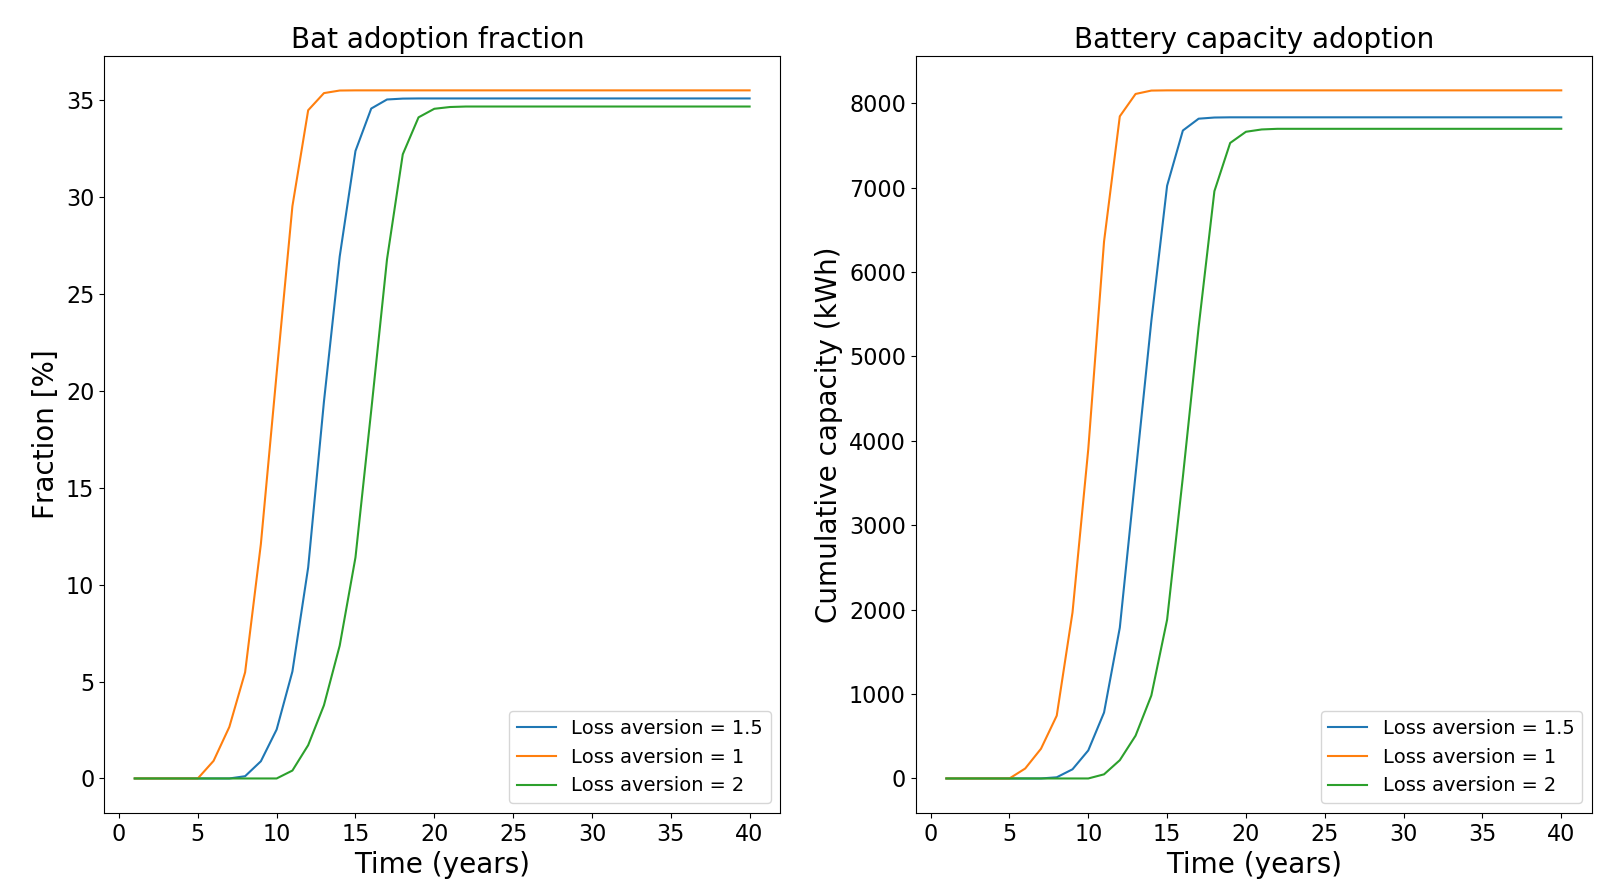
\includegraphics[width=12cm]{ModelAnalysis/Batloss.png}
\caption{Battery adoption for different loss aversions}
\label{Figure:batlossvol}
\end{figure}
\noindent
The battery adoption shows a similar trend as the PV adoption: for the lower loss aversion, the adoption of the technologies happens earlier and to a higher cumulative capacity level. The higher loss aversions will cause the adoption to occur later and at much lower levels. Contrary to the PV data, however, the adoption fraction will also vary as a function of the loss aversion. This analysis shows that the adoption of capital goods like PV panels and batteries are susceptible to a variation in loss aversion. Indeed, when thinking about the connotation of loss aversion, it stands to logic that actors showing high loss aversion will be less likely to invest in these technologies. This effect can be further seen in the configuration distribution, which is presented in Figure \ref{Figure:configlossvol}. 
\begin{figure}[h!]
\centering
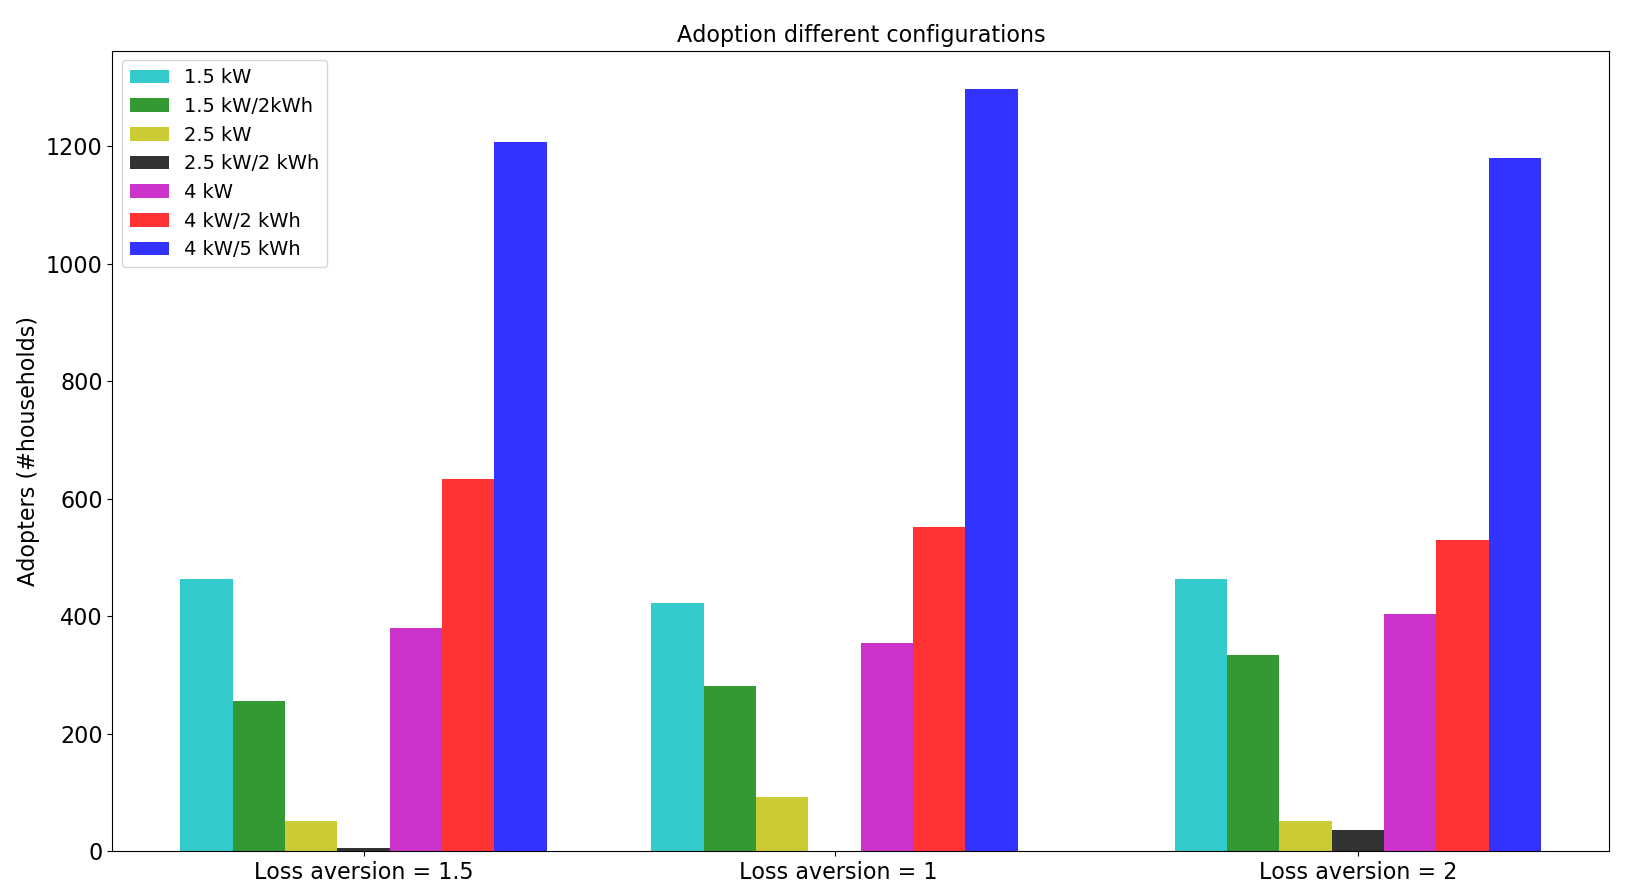
\includegraphics[width=12cm]{ModelAnalysis/Config.png}
\caption{Configurations for different loss aversions}
\label{Figure:configlossvol}
\end{figure}
\noindent
In accordance with the PV and battery adoption rates, the adoption of different configurations shows a slight difference for the different values of the loss aversion. The lower loss aversion values will make the most expensive technology ($4kW/5kWh$) the most popular. Concurrently, the less expensive technologies become less popular. For the higher loss aversion, the opposite will apply: large configurations become less popular whereas small configurations become more popular. The 1.5\textit{kW}/2\textit{kWh} in particular will be more popular for the higher loss aversion. 
\newline \newline \noindent
The utility death spiral that will result from this variation in the loss aversion can be found in Figure \ref{Figure:distlossvol}. Since the adoption happens earlier for the low loss aversion and later for the higher loss aversion, the utility death spiral will manifest itself accordingly.  
\begin{figure}[h!]
\centering
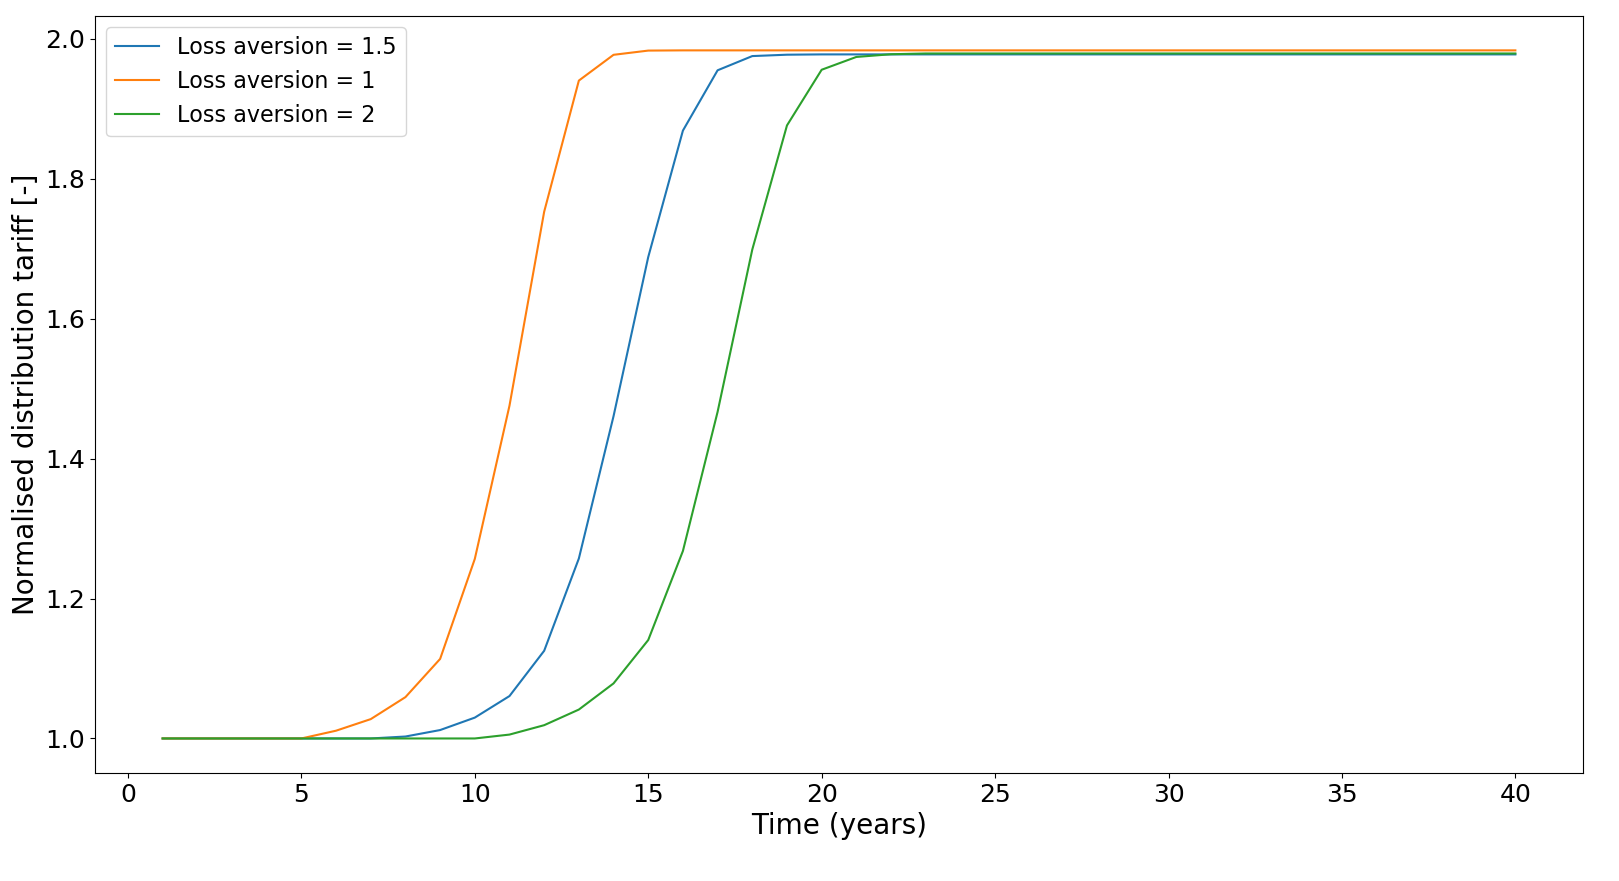
\includegraphics[width=10cm]{ModelAnalysis/Dist.png}
\caption{Distribution cost for different loss aversions}
\label{Figure:distlossvol}
\end{figure}
\noindent
Since CPT is not yet operationalizable as a decision-making theory, performing a sensitivity analysis of the loss aversion is not frequently done. Inversely, obtaining values for the loss and risk aversion will be the ultimate goal of most of the research in this field of research. This analysis, nevertheless, serves as a "stress test" to the model to control whether using the CPT makes sense in this setting. From the results discussion in this setting, there is a clear effect of the loss aversion coefficient on the adoption data. Since these results show a consistent trend for all configurations and technologies, this sensitivity analysis showed how research into CPT as a decision-making theory for simulating DER adoption in a consumer-centric energy system can be add valuable insights. 
%\subsection{Residual load}
%Since the utility death spiral depends on the amount of revenue changes the DSO has to recuperate when a portion of its customers start adopting DER, the residual load of the environment will be the driving force behind this utility death spiral. The higher the residual load as a fraction of the total load, the more recurring revenue the DSO can rely on. This will make it easier for the DSO to pay for all the costs he must incur to maintain and upgrade his infrastructure. A lower residual load, however, will force the DSO to increase his tariffs more to maintain his revenue. The extent of a difference in residual load will be discussed in the subsequent paragraphs. Besides the standard residual load case, where $Resid.\: load = Repl. \:load$, two additional scenarios will be tested. The first one will be for a lower residual load ($Resid. \: load = 0.33*(Repl.\: load)$) and a higher residual load  ($Resid. \: load = 3*(Repl. \: load)$)
%\newline \newline \noindent
%The PV adoption for different residual load cases can be found in Figure \ref{Figure:pvresid}. 
%\begin{figure}[h!]
%\centering
%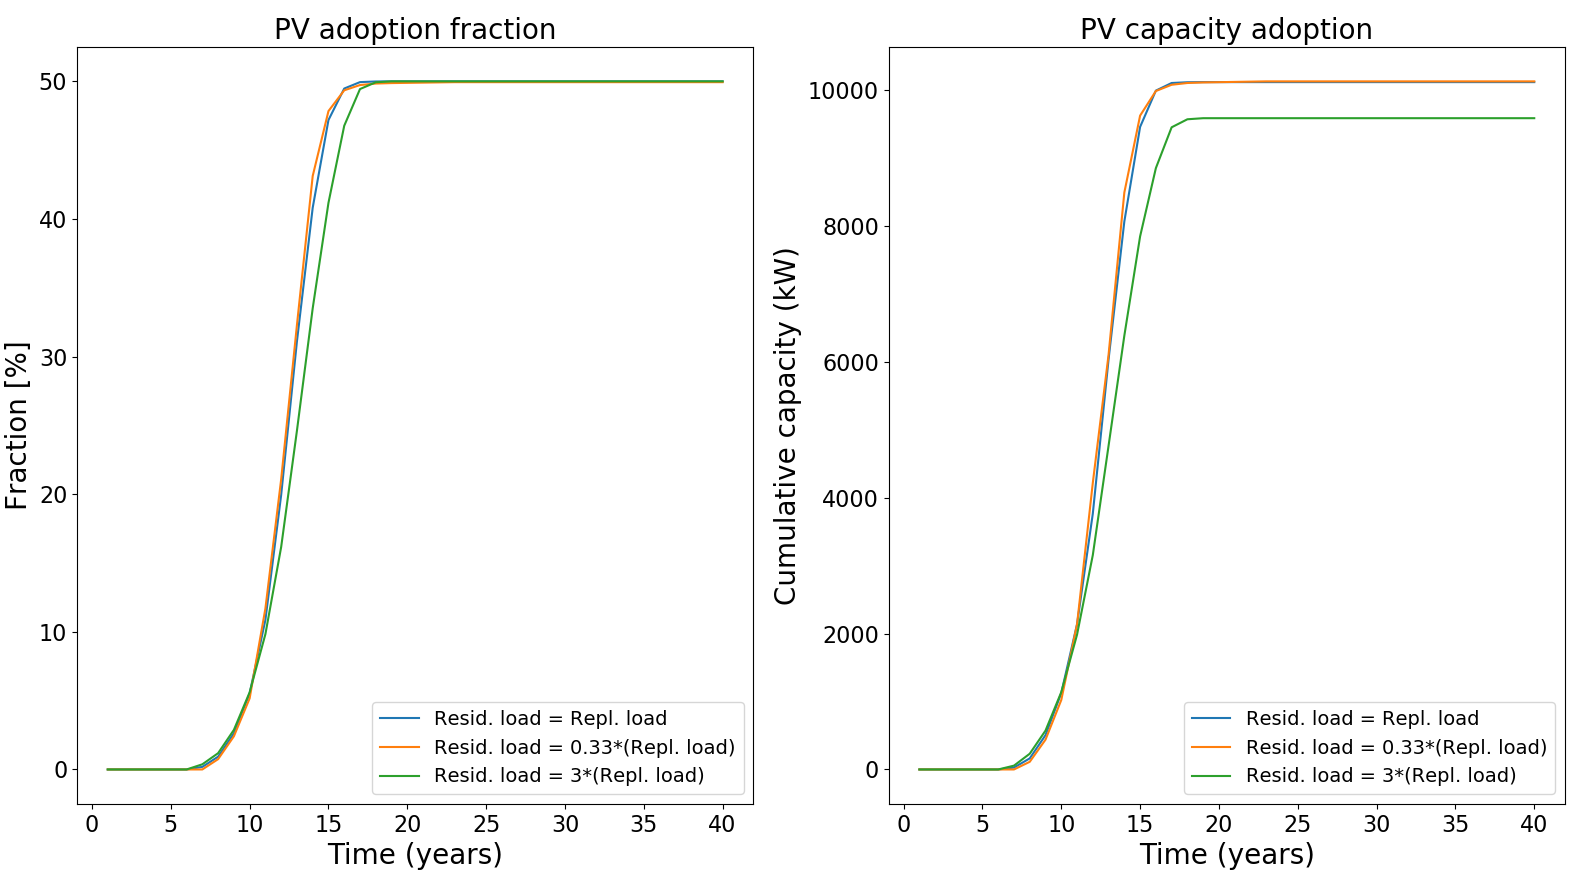
\includegraphics[width=12cm]{ModelAnalysis/PVresid.png}
%\caption{PV adoption for different residual loads}
%\label{Figure:pvresid}
%\end{figure}
% \noindent
%Here, the effect of different residual loads is quite subtle. The results for the three residual loads are quite similar, both in adoption fraction and in cumulative PV capacity adopted. The only exception is the cumulative PV capacity for the higher residual load, which will be slightly lower due to the lower savings. This also applies to the battery technology, although the cumulative capacity does show some more variation, as can be seen in Figure \ref{Figure:batresid}. For both technologies, the cumulative adopted capacity for the higher residual load will be lower since the savings will be lower. These savings will be lower because the DSO will have less recurring revenue to rely on, which will force him to adapt his tariffs more rapidly. For the higher residual load, the opposite effects will play. 
%\begin{figure}[h!]
%\centering
%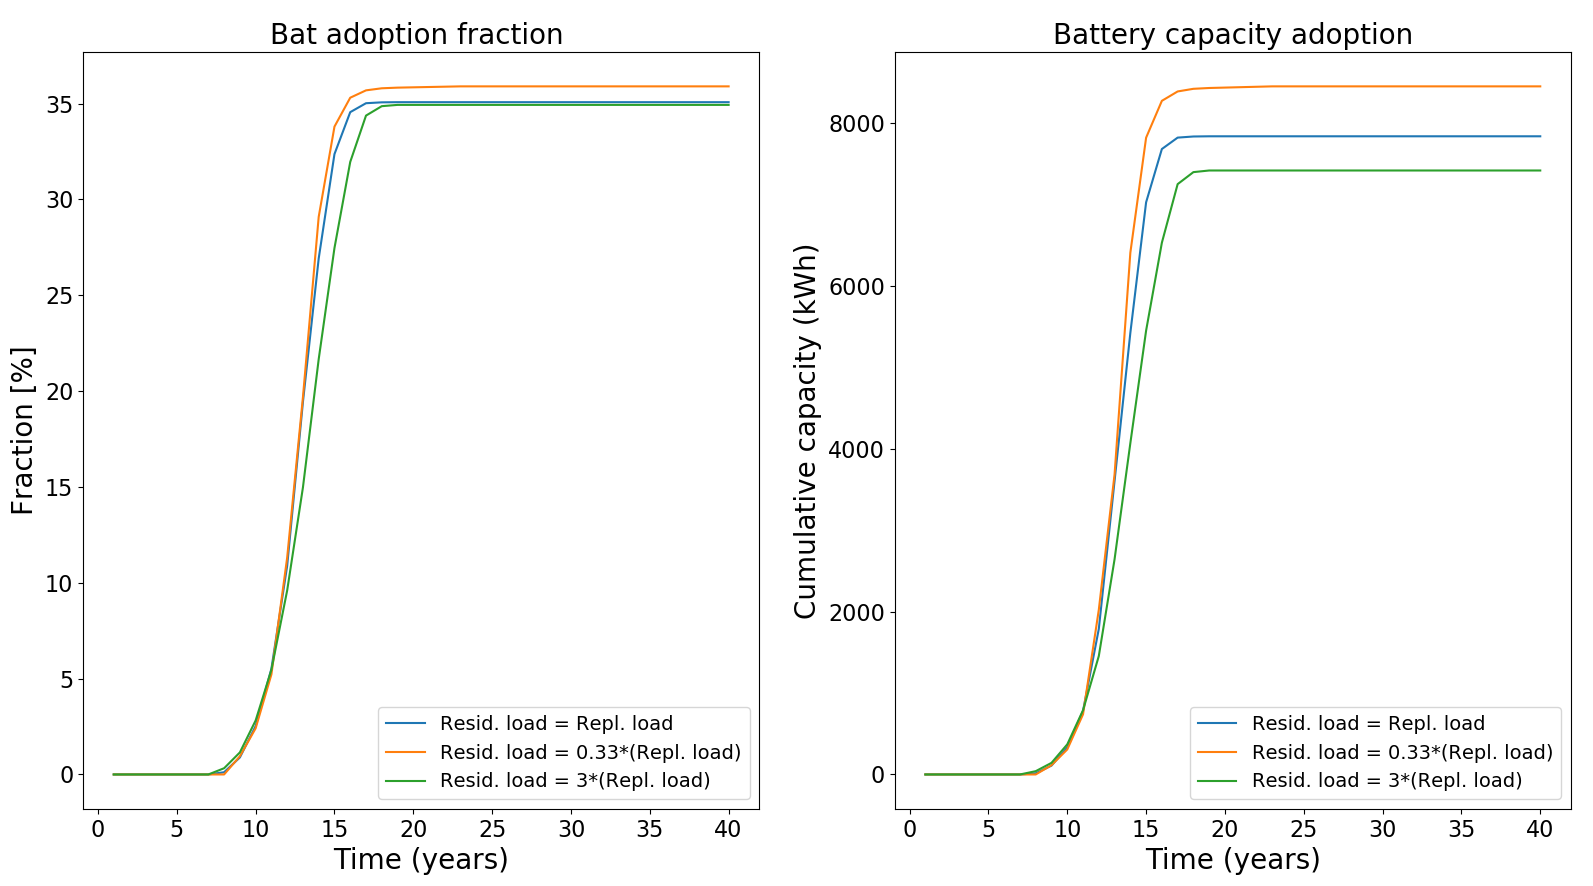
\includegraphics[width=12cm]{ModelAnalysis/BatResid.png}
%\caption{Battery adoption for different residual loads}
%\label{Figure:batresid}
%\end{figure}
 %\noindent
%The resulting configuration distribution can be seen in Figure \ref{Figure:configresid}. Here, the effect of different residual loads becomes more visible. For the lower residual loads, which translates into higher tariffs and savings, the largest configuration (4\textit{kW}/5\textit{kWh}) will become more popular. For the higher residual load, the tariffs and savings will be lower, making this configuration less popular. In fact, the change in battery adoption that can be seen in Figure \ref{Figure:batresid} is mainly due to the variation of this 5\textit{kWh} configuration.
%In addition to the largest configuration, the variation of the residual load will also have an effect on smaller configurations, most notably the 1.5\textit{kW}/2\textit{kWh} installation. Contrary to the larger configurations, this one will become more popular in the high residual load case, when savings are lower, while being less popular in the low residual load case, when savings are higher. The resulting distribution tariff can be found in Figure \ref{Figure:distresid}. In parallel with the adoption levels, the distribution tariff will increase by more than 300\% in the low residual load case, while this increase will only be 33.1\% in the case of a higher residual load. 
%\begin{figure}[h!]
%\centering
%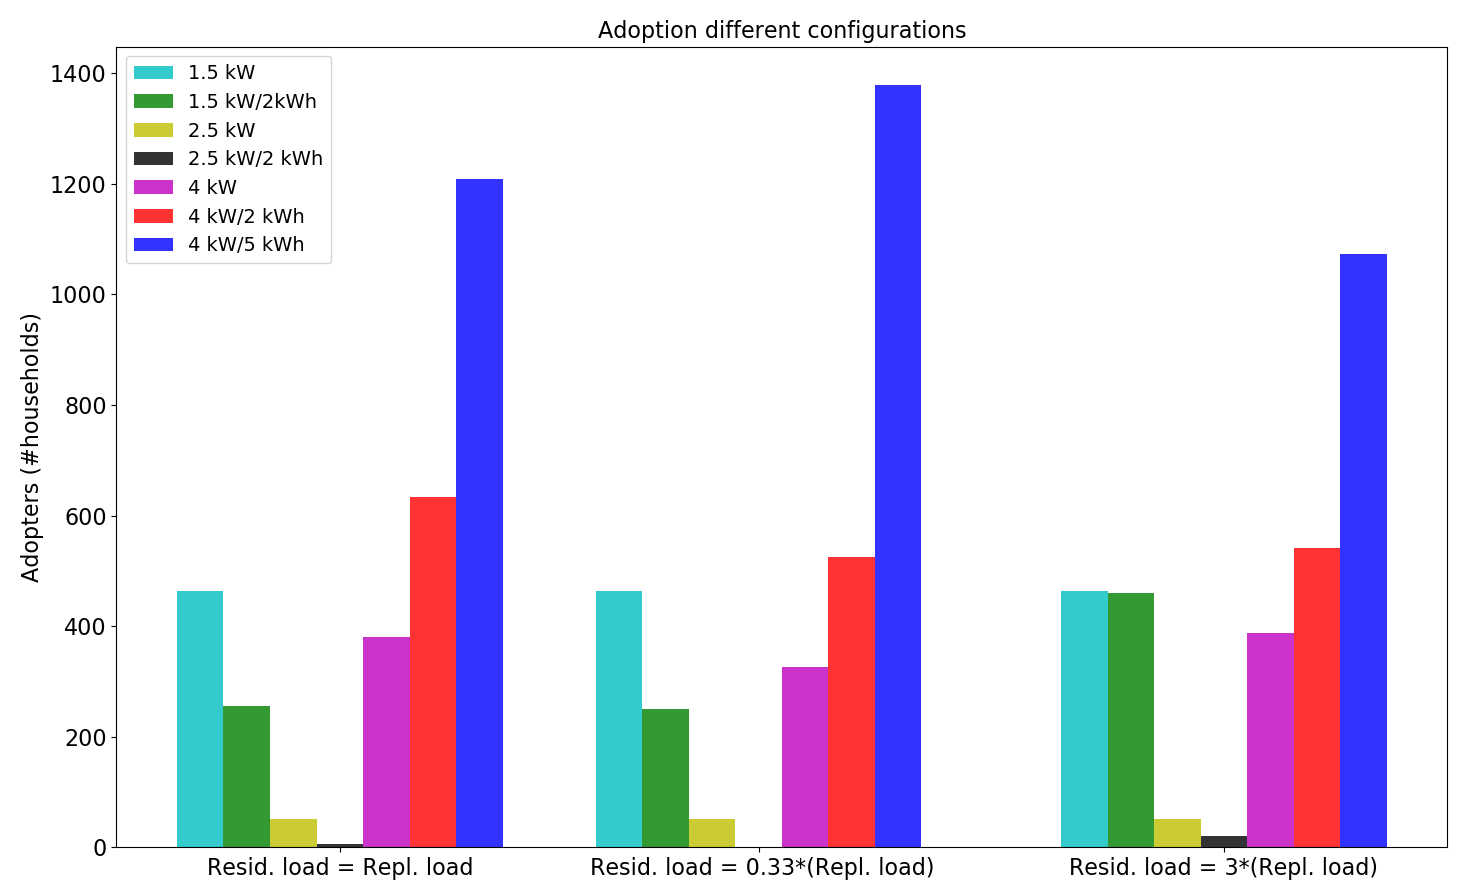
\includegraphics[width=12cm]{ModelAnalysis/ConfigResid.png}
%\caption{Configurations for different residual loads}
%\label{Figure:configresid}
%\end{figure}
% \noindent
 %The resulting configuration distribution can be seen in Figure \ref{Figure:configresid}. Here, the effect of different residual loads becomes more visible. For the lower residual loads, which translates into higher tariffs and savings, the largest configuration (4\textit{kW}/5\textit{kWh}) will become more popular. For the higher residual load, the tariffs and savings will be lower, making this configuration less popular. In fact, the change in battery adoption that can be seen in Figure \ref{Figure:batresid} is mainly due to the variation of this 5\textit{kWh} configuration.
%In addition to the largest configuration, the variation of the residual load will also have an effect on smaller configurations, most notably the 1.5\textit{kW}/2\textit{kWh} installation. Contrary to the larger configurations, this one will become more popular in the high residual load case, when savings are lower, while being less popular in the low residual load case, when savings are higher. The resulting distribution tariff can be found in Figure \ref{Figure:distresid}. In parallel with the adoption levels, the distribution tariff will increase by more than 300\% in the low residual load case, while this increase will only be 33.1\% in the case of a higher residual load. 
%\newline \newline \noindent
%The resulting distribution tariff can be found in Figure \ref{Figure:distresid}. In parallel with the adoption levels, the distribution tariff will increase by more than 300\% in the low residual load case, while this increase will only be 33.1\% in the case of a higher residual load.  
%\begin{figure}[h!]
%\centering
%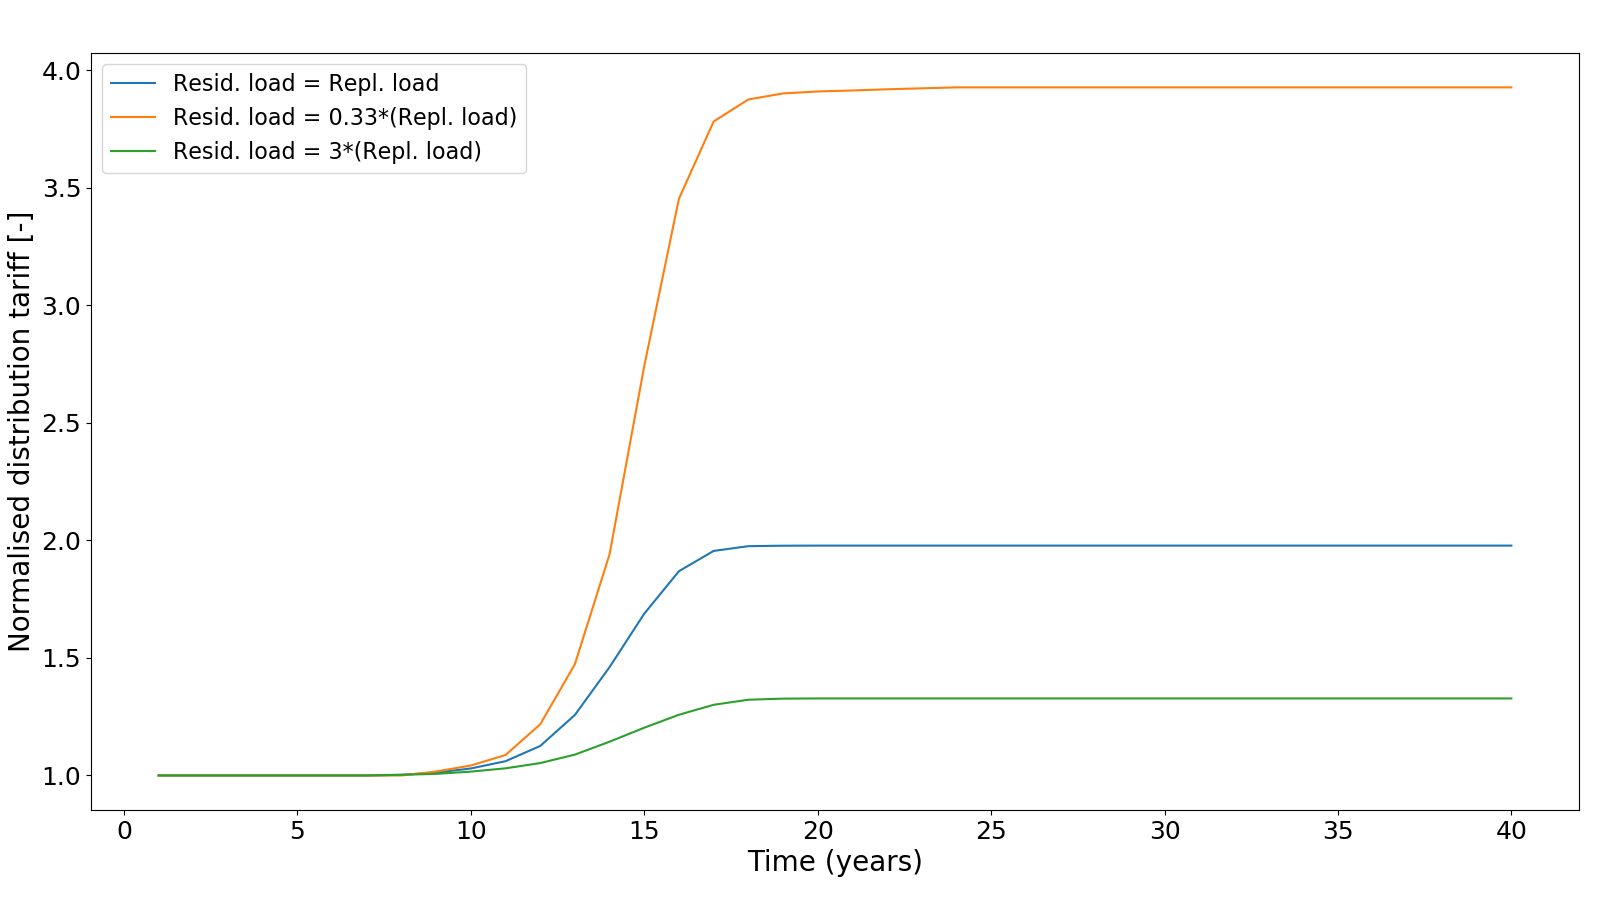
\includegraphics[width=10cm]{ModelAnalysis/distresid.png}
%\caption{Distribution tariff for different residual loads}
%\label{Figure:distresid}
%\end{figure}
%\noindent
%Judging by the data presented in this section, the residual load has an effect on the adoption of certain configurations. Most notably, the adoption of the 1.5\textit{kW}/2\textit{kWh} and 4\textit{kW}/5\textit{kWh} configurations will change as a function of the residual load. This is mainly due to the effect of a change in the network charge on the savings. The lower the residual load, the more popular the large configurations and the less popular the small configurations will be. The higher the residual load, the more popular the smaller configurations are and the less popular the larger configurations. This adoption shift between different configurations will cause the effect on the aggregate adoption fraction and capacity adopted to be rather limited, with the exception of the battery capacity adopted. In parallel with the DER evolution, the network charges will increase in the utility death spiral process. 
\subsection{Battery subsidies}
Since the battery subsidy can decrease the capital requirements for a battery, this incentive could make the technology significantly more popular. An analysis of how different subsidy levels can have an influence on the adoption levels can provide additional insights into this specific policy. Since the policy used in this Thesis is based on the program of the Flemish government for residential battery subsidies, the base case value is 250 \EUR{}/\textit{kWh}. Battery costs, though, are decreasing rapidly and are expected to continue to do so in the future (see Figure \ref{Figure:bloom}). This will most likely cause subsidies to decrease. The different battery subsidy levels that will be tested, therefore, are 150 \EUR{}/\textit{kWh} and 50 \EUR{}/\textit{kWh}.
The PV adoption data for the different subsidies can be found in Figure \ref{Figure:PVsubsvol}:
, \ref{Figure:batsubsvol}, \ref{Figure:configsubsvol} and \ref{Figure:distsubvol}. 
\begin{figure}[h!]
\centering
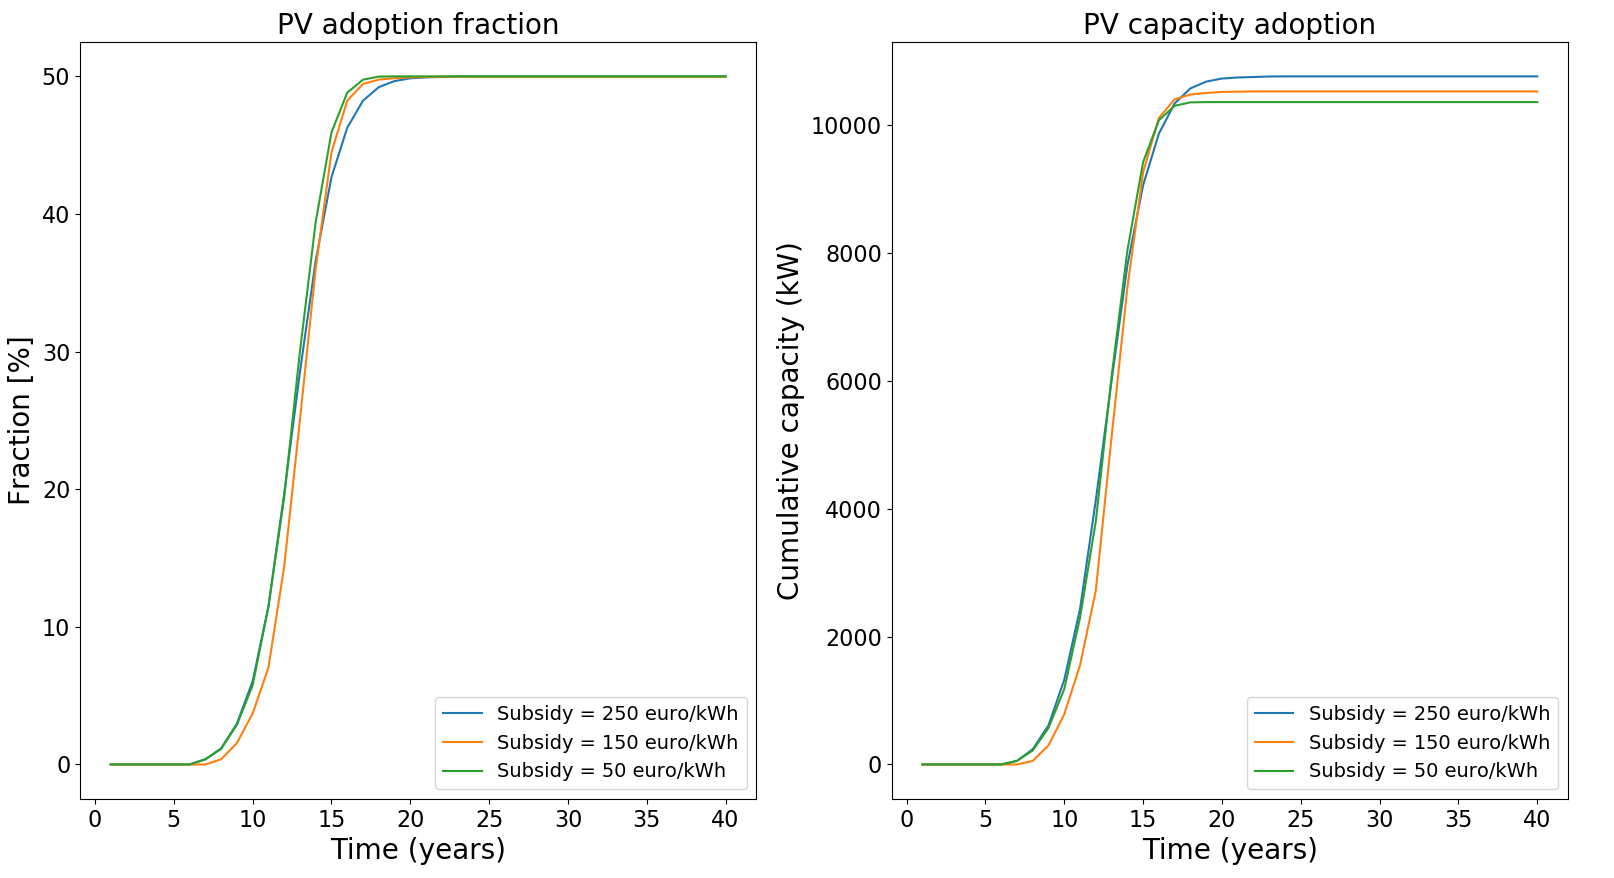
\includegraphics[width=12cm]{ModelAnalysis/PVsubs.png}
\caption{PV adoption for different battery subsidies}
\label{Figure:PVsubsvol}
\end{figure}
 \noindent 
Interestingly, the higher subsidies do not show a visibly higher adoption of PV adopters or capacity. Since higher battery subsidies make the capital costs and payback period of several configurations lower, this should make the adoption incentive for PV-battery systems and PV panels themselves higher. The data in Figure \ref{Figure:PVsubsvol},  however, shows that the difference between the different policies is small. As will become clear from Figure \ref{Figure:configsubsvol}, this is mainly due to a shift in preferences among the three different 4\textit{kW} configurations, which will cause the overall adopted PV capacity to change very little. Between the highest and lowest subsidy, the difference in PV capacity adopted is 3.9\% . 
\begin{figure}[h!]
\centering
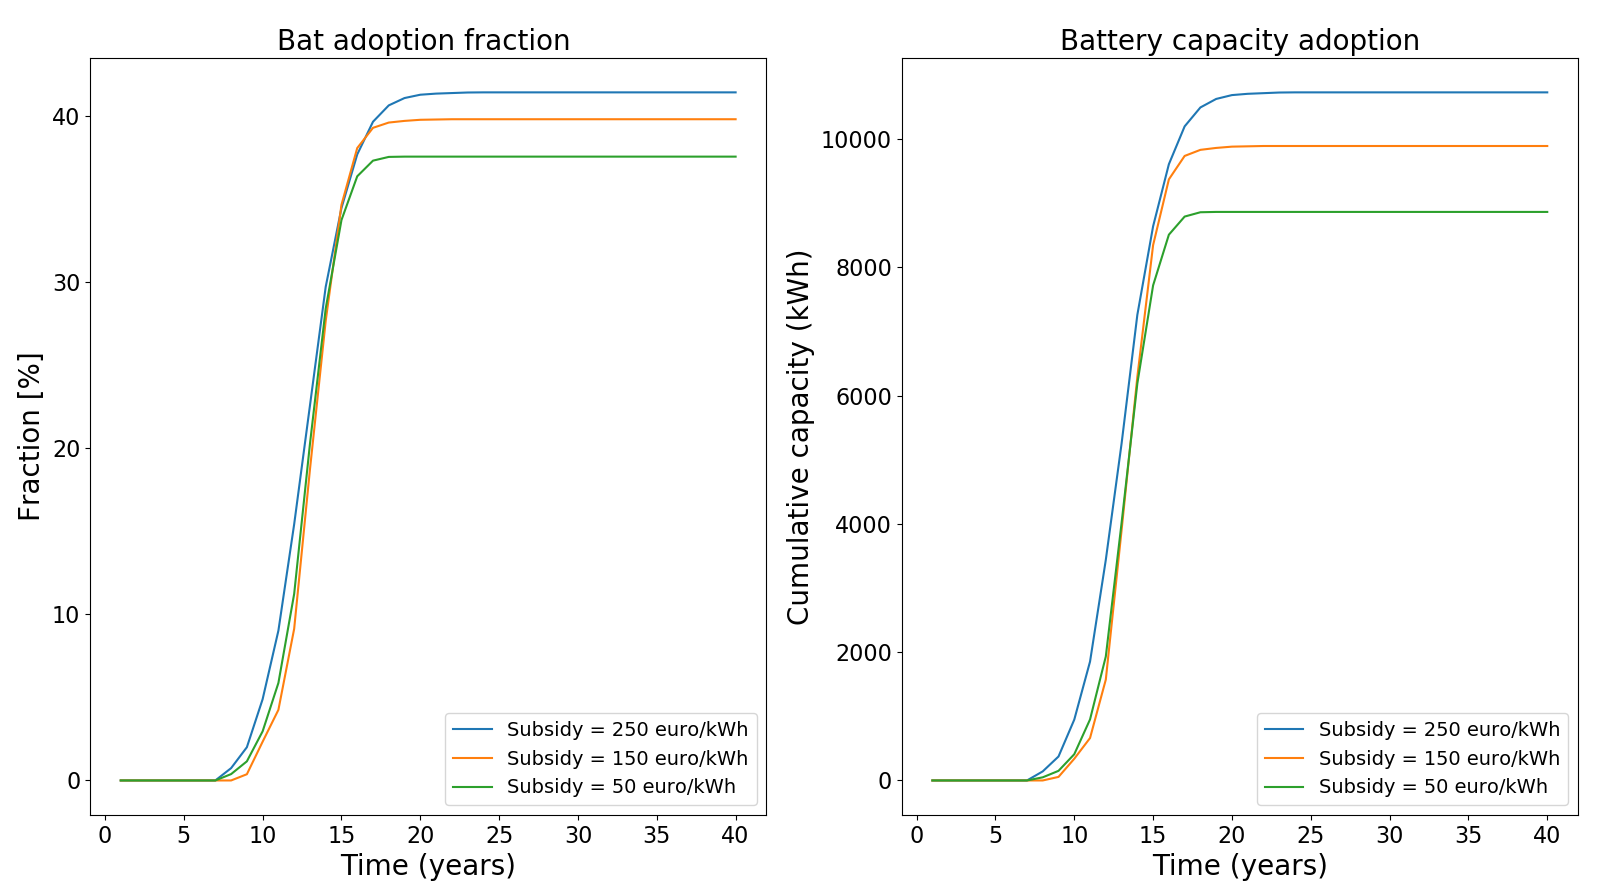
\includegraphics[width=12cm]{ModelAnalysis/Batsubs.png}
\caption{Battery adoption for different subsidies}
\label{Figure:batsubsvol}
\end{figure}
 \noindent
Contrary to the PV results, the battery subsidies show a very clear effect on the battery adoption data, as can be found in Figure \ref{Figure:batsubsvol}. The higher subsidies, the higher the adoption fraction and adopted capacity. The number of adopters for the \EUR{} 150 subsidy is 4.4\% lower than the case while being 9.9\% lower for the \EUR{} 50 subsidy. For the 150 \EUR{} option, the adopted capacity will be 7.5\% lower than in the base case, while for the 50 \EUR{} option, the adopted capacity will be 18.6\% lower than the base case. Both the adoption fraction and the adopted capacity are, therefore, increasing with an increasing subsidy. As can be seen from Figure \ref{Figure:configsubsvol}, one main trend will shape this adoption. 
\begin{figure}[h!]
\centering
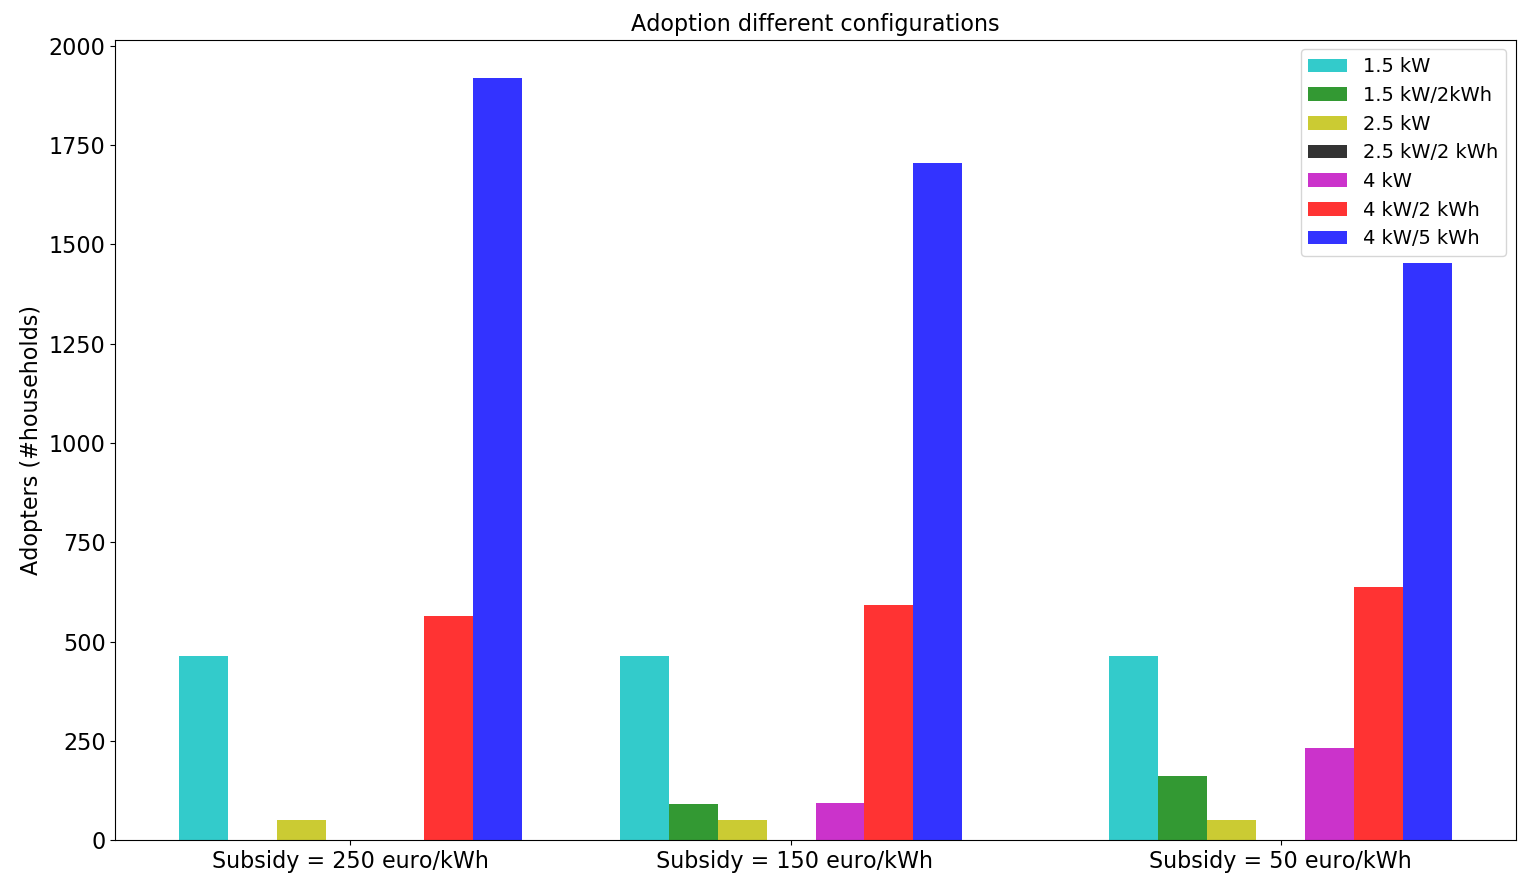
\includegraphics[width=12cm]{ModelAnalysis/Configsubs.png}
\caption{Configurations for different subsidies}
\label{Figure:configsubsvol}
\end{figure}
 \noindent
 The higher the subsidies, the more the adoption will focus on the \textit{4kW/5kWh} configuration. 
Since this configuration will experience the effect of the subsidies fivefold (since a \textit{5kWh} battery is installed), this technology will become disproportionately popular (note how the 4\textit{kW}/2\textit{kWh} adopters even decrease for higher subsidies). The other configurations will be less popular since the subsidy effects are less present. In parallel with the adoption levels, the distribution tariff evolves to higher levels for the lowest subsidies, since the PV adoption levels are the highest for this specific policy. For the higher subsidies, the PV adoption is higher, causing the utility death spiral to manifest itself to a fuller extent.  
\begin{figure}[h!]
\centering
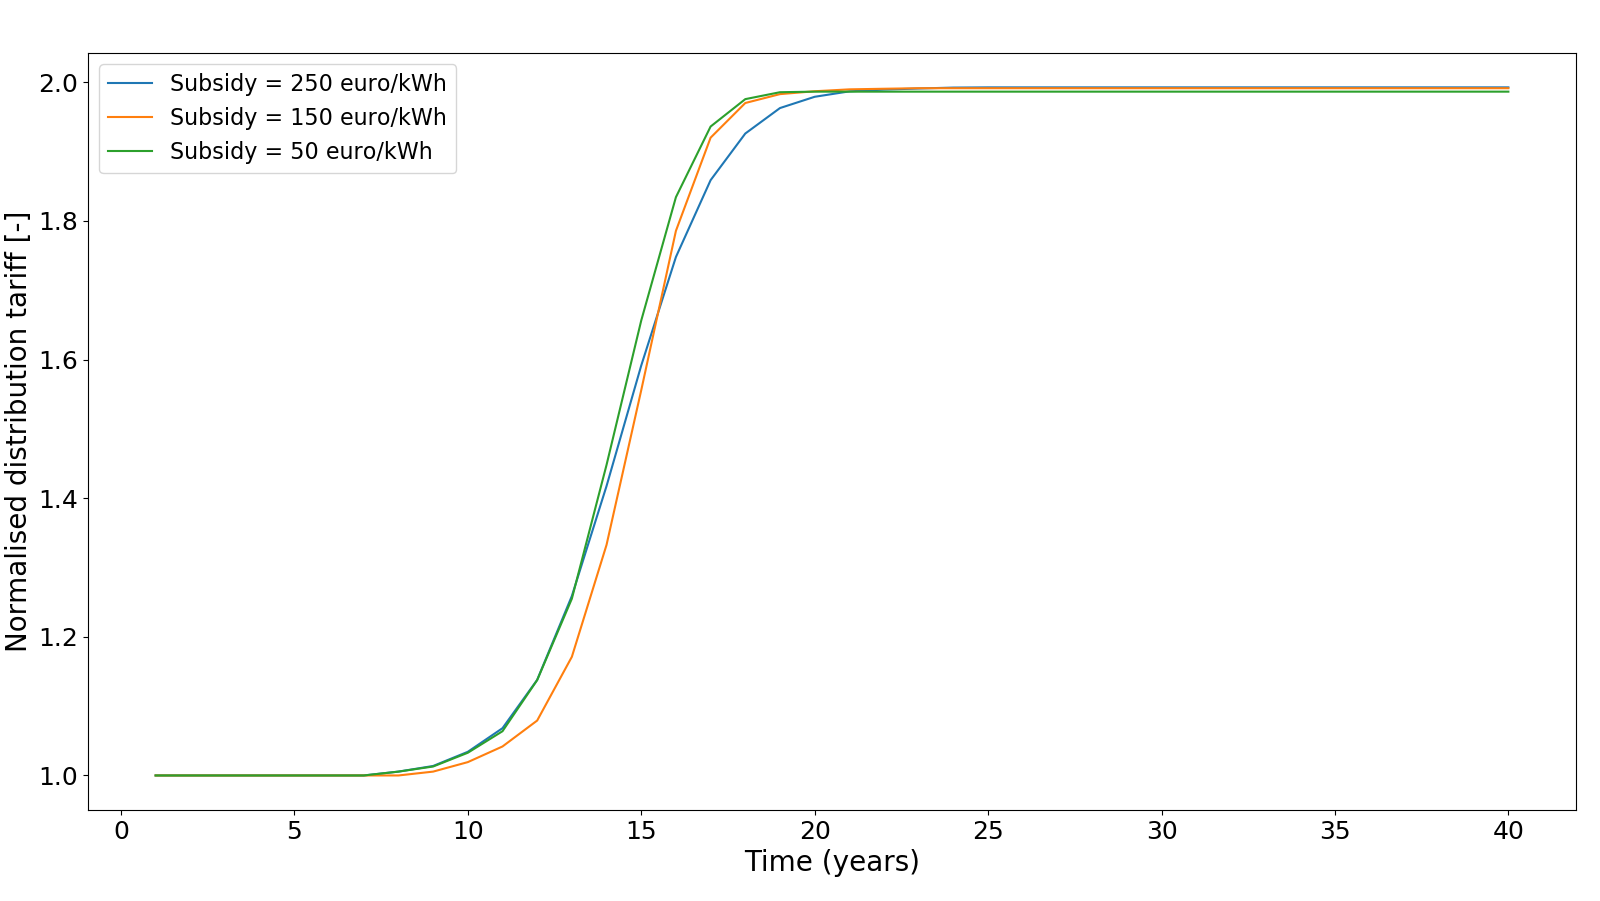
\includegraphics[width=6cm]{ModelAnalysis/Distsubs.png}
\caption{Distribution cost for different subsidies}
\label{Figure:distsubvol}
\end{figure}
 \noindent
Higher battery subsidies will, therefore, cause the adoption of the largest PV/battery systems to be encouraged. Lower subsidies can still encourage higher battery adoption without causing the adoption to be focused on one single configuration.
%\subsection{Network charge}
%\label{distanal} As was already discussed in Section \ref{compar}, the different network charges have a different effect on the savings and, therefore, the overall adoption and subsequent utility death spiral. The main driver for this difference in adoption between the net volumetric tariff and annual capacity offtake tariff is the difference in savings between the two tariffs. Both the way in which savings are created as well as the effect of this change in savings on the adoption of DER will be discussed in the next few paragraphs.
%\newline \newline \noindent
%Since the savings for a household due to the adoption of DER consist of both energy costs and (some) distribution costs, the overall savings will evolve with these components. In the case of the net volumetric distribution tariff, the distribution component can be calculated using Equation \ref{distnet}. This cost formula suggest that the savings of the household can increase substantially in case $q_{net}$ reaches a value close to zero. As can be seen in Figure \ref{Figure:netdem}, $q_{net}$  of all but two configurations is equal to zero, meaning that all distribution charges are avoided. Compared to $q_{net}$ for no DER adoption, the savings of the distribution component and by extension the electricity cost are significant. 
%\begin{figure}[h!]
%\centering
%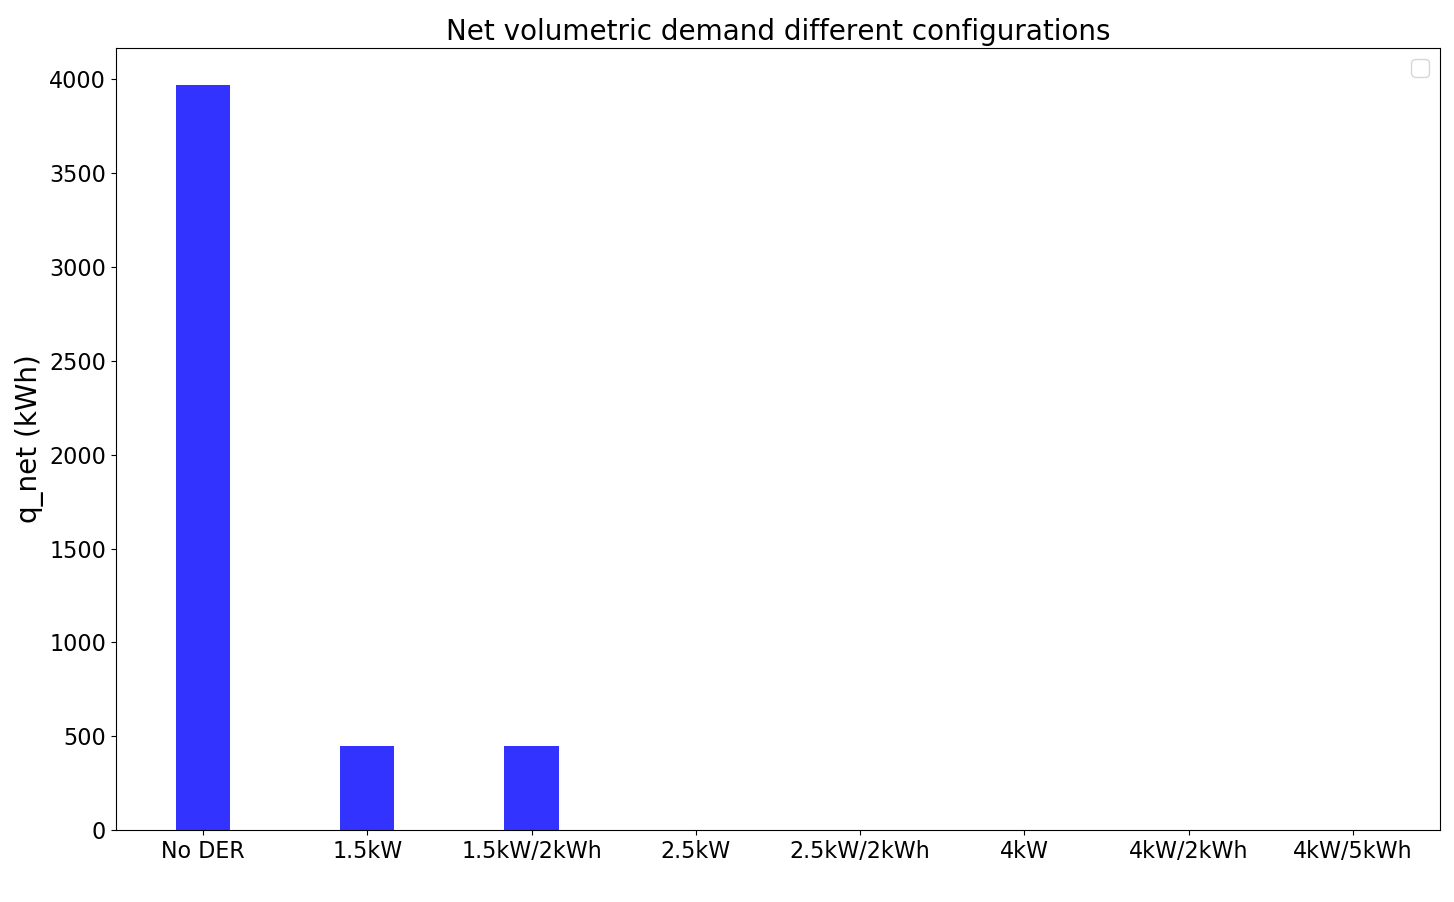
\includegraphics[width=12cm]{ModelAnalysis/Netdemand.%png}
%\caption{Net volumetric demand for different DERs %configurations}
%\label{Figure:netdem}
%\end{figure}
%\noindent
%For the annual capacity offtake tariff, the distribution cost can computed using Equation \ref{qcap}. This network charge formulation suggests that, like in the volumetric case, the distribution cost could decrease to zero. When looking at Figure \ref{Figure:peakdem}, however, it becomes clear that $q_{cap}$ and the distribution cost component will remain strictly positive for all configurations.  
%\begin{figure}[h!]
%\centering
%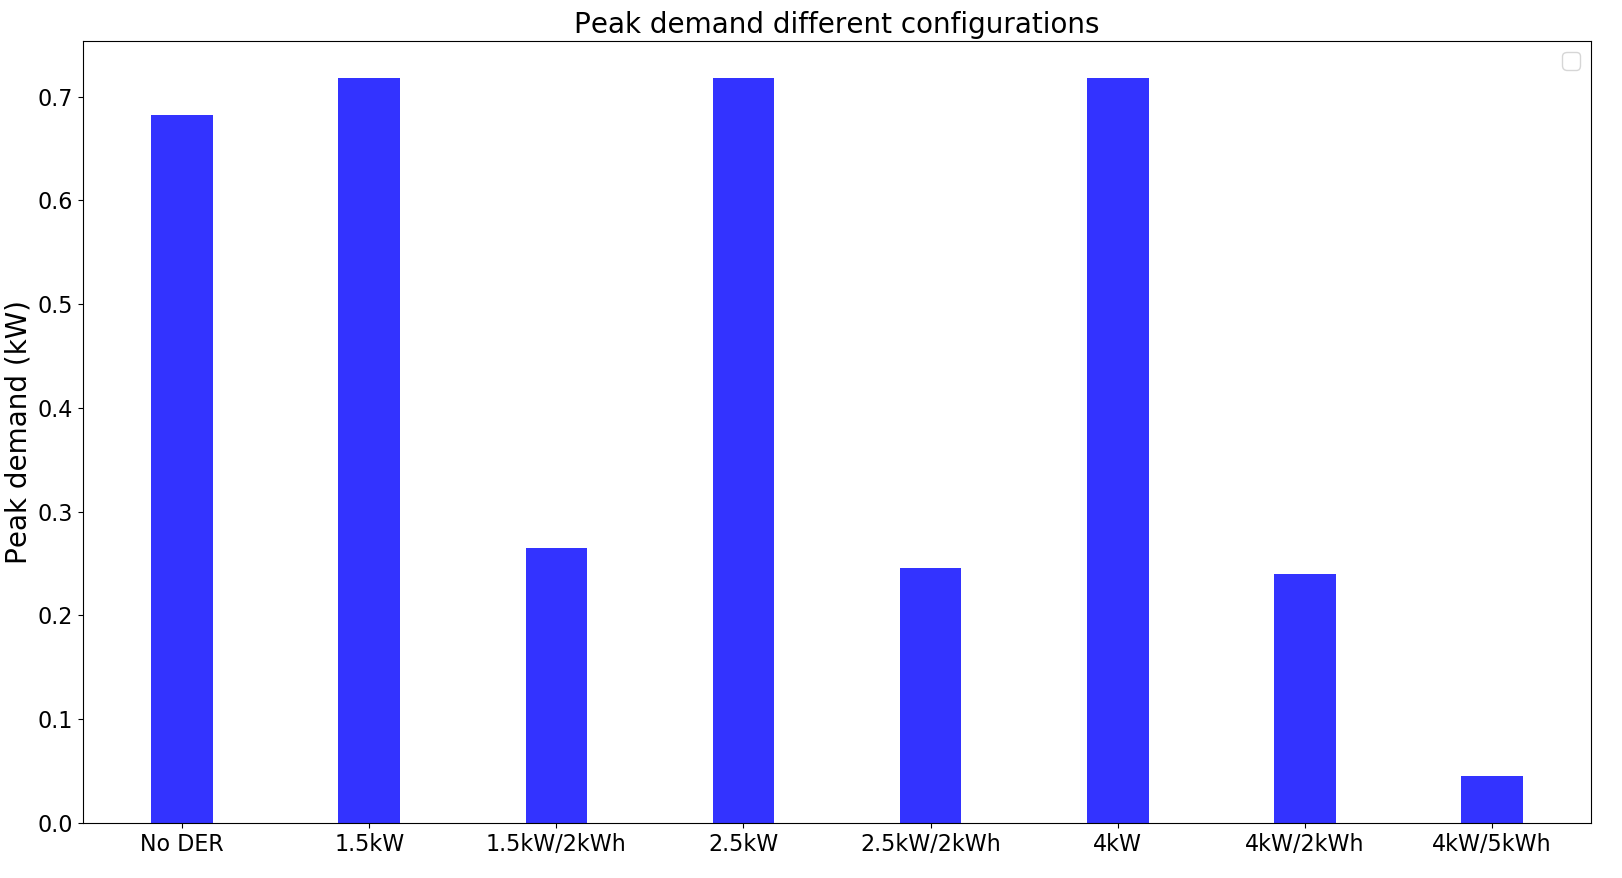
\includegraphics[width=12cm]{ModelAnalysis/PeakDemand.png}
%\caption{Different peak demands}
%\label{Figure:peakdem}
%\end{figure}
%\noindent
%Due to the previously discussed difference in distribution cost for the two different network charges, the savings will de different, as can be seen in Figure \ref{Figure:Savings} \footnote{The represented data is the average of the savings for all configurations}. Here, it can be seen how the savings realised in the case of the net volumetric distribution tariff are much higher than for the annual capacity offtake tariff. Besides having a larger initial value, the savings for the volumetric network charge also increase more streadily than those in the capacity tariff case: the volumetric savings increase by 39.6\% throughout 40 year simulation, whereas they only increase by 6.8\% in the capacity case pver the same period. This is a direct result of the higher initial value in the volumetric distribution tariff case: the higher savings cause a higher adoption incentive, causing the utility death spiral to manifest itself more clearly, which will cause the distribution tariff to increase further. The results discussed in Section \ref{compar} showed the extent of this utility death spiral for the different policies. 
%\begin{figure}[h!]
%\centering
%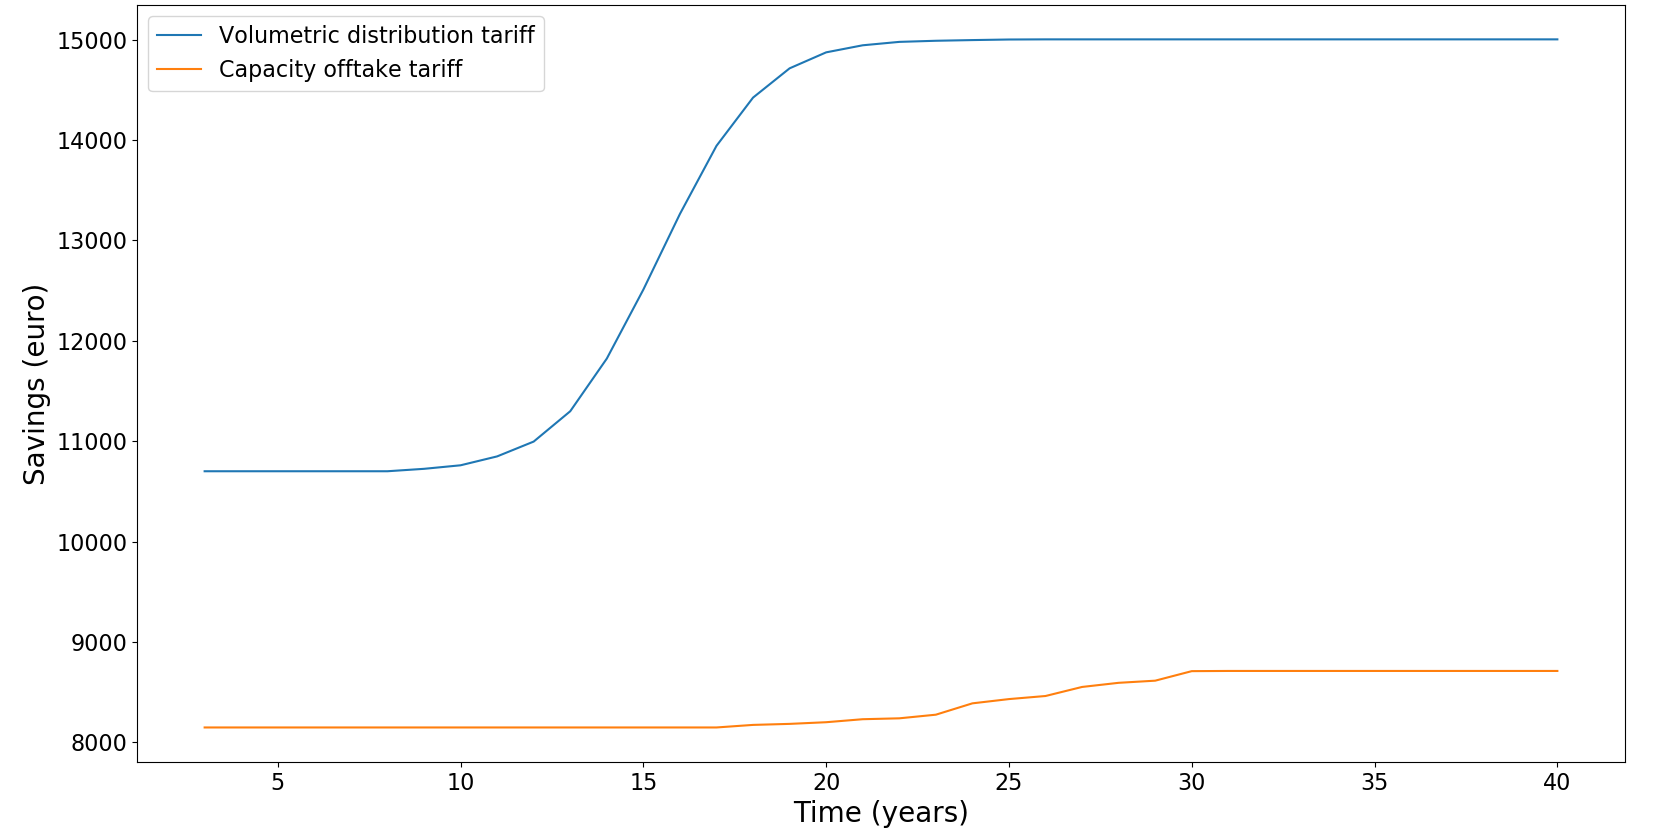
\includegraphics[width=12cm]{ModelAnalysis/Savings.png}
%\caption{Savings for the volumetric and capacity tariff}
%\label{Figure:Savings}
%\end{figure}
\subsection{Preliminary analysis \& Conclusion}
Given the analysis of different parameters in the model, several conclusions can be drawn on a preliminary basis. First and foremost, the sensitivity analysis of the loss aversion showed how the adoption data can vary. A lower loss aversion causes the adoption to kick off sooner, while a higher loss aversion will have the opposite effect. Given the consistency of these results, further research into CPT as a decision-making theory in the DER adoption process could add valuable insights. 
%What also became clear from this analysis, is the role of the residual load in the DER adoption process. Since a lower residual load causes the network charges and savings to be higher, the incentive to adopt DER becomes higher, thereby reinforcing the network charge increase once again, creating a vicious circle. Currently, the fraction of DER in the overall electricity landscape still is limited, but rising quickly. Over the next few decades, as policy makers intend to make a large portion of the households adopt DER to reduce emissions, the residual load will become a smaller portion of the overall load, which would cause the utility death spiral effects to be amplified. The distribution cost evolution for low residual loads that was presented in Figure \ref{Figure:distresid} could, therefore, materialize over the next few decades if appropriate action is not taken. As was discussed in Section \ref{compar}, the capacity-based network charge can mitigate these effects. The main reason for this, as was discussed in Section \ref{distanal}, is the change in the distribution cost component and its effects on the savings and adoption incentive. For the net volumetric distribution tariff, this cost component decreases to zero for most configurations, generating more savings to the households and encouraging DER adoption. The design of the capacity offtake tariff, however, will cause the distribution component to decrease by a smaller amount for most configurations, generating less savings to the households, thereby encouraging DER adoption to a lesser extent. 
\newline \newline \noindent
Battery subsidies can help enhancing the adoption of batteries. Higher subsidies result in a higher cumulative PV capacity, higher battery adoption fraction and significantly higher cumulative battery capacity. The main driver for this increase in adoption and capacity is the increased popularity of the 4\textit{kW}/5\textit{kWh} configuration. It is, therefore, questionable if the battery subsidy should be that high, since this configuration will cause a lot of grid injection and grid stability issues. More fundamentally, though, the question is whether battery subsidies are necessary altogether. Since the battery adoption fraction increases from 37.3\% to 41.4\% for the lowest to the highest subsidy (see Figure \ref{Figure:batsubsvol}), the efficiency of these subsidies is questionable. Since the cumulative capacity increases from about 8,600 to 10,600 \textit{kWh}, the subsidies increase from \EUR{} 430,000 to \EUR{} 2,650,000. This 516\% increase in subsidies for a 23.2\% increase in battery capacity and an 11\% increase in adoption seems like a waste of government resources. These subsidies are to be monitored closely and reduced significantly once battery costs decrease and the adoption rates start increasing, since a continuation of these subsidies could be financially wasteful. 
\newline \newline \noindent
Next to the insights gathered in this section, the analysis of different parameters embedded in the model also gives rise so several points of attention. The most important one also relates to the loss aversion. In this Thesis, the used value is the one that based on the measurements performed by Bougherare et al. \cite{lossaversions}, which was set at $\lambda = 1.5$. However, since this value is the result of experimental data, just like the values measured by Kahneman and Tversky, the transposition of the loss and risk aversion value to this Thesis is an assumption that is to be validated by performing field experiments with energy prosumers being the target. As the sensitivity analysis showed, a variation of the loss aversion causes the results to vary significantly. An incorrect estimate of the loss aversion could, therefore, cause the results to deviate significantly. 
\newline \newline \noindent
In addition, the analysis of the battery subsidies was done under the current projections for cost decrease. Since battery technology currently is in a period of rapid growth, the development of this DER can follow many different paths. A sudden change in technology or policies could, therefore, discredit the results discussed in this Thesis. In addition, the combination of constant subsidies throughout the simulation combined with the cost reduction of the battery technology could give a rather optimistic view on the battery adoption.
\newline \newline \noindent
Note that this list of parameters susceptible to a sensitivity analysis is not comprehensive. Note that one important parameter that needs further analysis in this context is the time value of money or discount factor $r$. As was discussed in Section \ref{Investmentss}, many of the characteristics of investments in DER are a function of time, like long-run uncertainties, long payback periods and investment postponement options. This makes the time preference of the investor important in the adoption process. In future work, therefore, different time preference and loss aversion configurations should be tested. 
\section{Comparison to EUT} \label{EUTcompar}
Since this Thesis uses CPT for the simulation of investments in DERs, a comparison to the most common decision-making theory, the EUT, can provide additional insights into the model. By comparing these two decision-making theories, the potential benefits or drawbacks of CPT over EUT can be discussed. This will be done for both the annual net metering and annual capacity offtake tariff. The other policies can be found in Appendix \ref{app:3}. 
\newline \newline \noindent
The decision variable for the EUT is the overall payback period of the different configurations (since this theory does not take into account a reference point of the current situation/level as CPT does). The utility of the payback period will be normalised according to the method proposed by Zhao et al. \cite{ABMPV}:
\begin{equation} \label{EUTnorms}
	NUT_{eco,i} = \frac{Max(UT) - UT_{i}}{Max(UT) - Min(UT)}
\end{equation}
Besides this difference, the implementation of the EUT in the ABM is identical to that of the CPT to guarantee both simulations are as comparable as possible. The analysis is, therefore, done on a "ceteris paribus" basis. In the following sections, the comparison of CPT with EUT will be done in the net metering case for both tariff structures.
\subsection{Annual net metering}
For the annual net metering policy, the PV adoption using EUT can be found in Figure \ref{Figure:PVeut}. This adoption shows an S-shaped adoption pattern, much like the CPT results do, except for the beginning of the adoption process. This shows that the adoption using EUT follows the sequence of innovators, early adopters all the way down to laggards, which corresponds to Rogers' theory of innovation and the results sequence of the CPT. Note that the final adoption fraction in the case of the EUT also is 50\%, meaning that all household that could have adopted DER have done so. Where the EUT simulation shows some significant differences with the CPT, as can be seen in Figure \ref{Figure:PVcompar}, is in the rate of adoption. 
%\begin{figure}[h!]
%\centering
%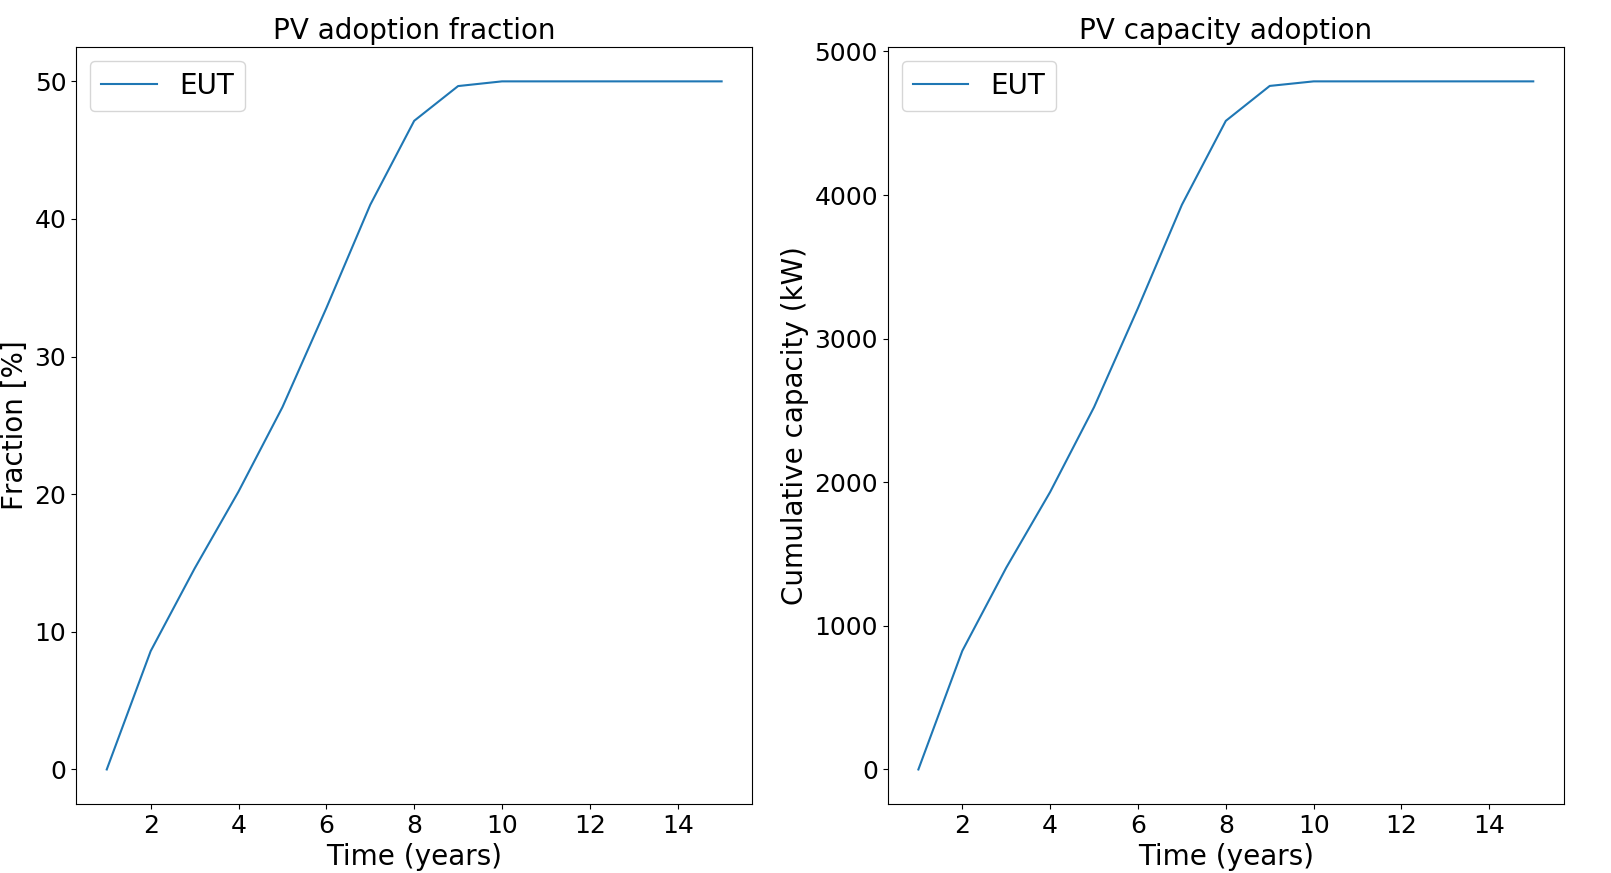
\includegraphics[width=12cm]{EUTCompar/PVEUT.png}
%\caption{PV adoption under EUT}
%\label{Figure:PVeut}
%\end{figure}
 %\noindent 
 Under CPT, the adoption is a gradual process where the technologies get adopted over a period of about 10 years. The adoption will also kick off in year 6-7, since the adoption threshold is only reached in this period. The EUT results, however, show an adoption process starting in year 1, followed by a very rapid adoption process to full adoption. Comparing the two simulations with each other, CPT does seem to create a more realistic simulation of the PV adoption process. Note that the adoption fraction is 50\% (i.e. full adoption) for both decision making theories, but the overall adopted capacity is higher for the CPT. This is mainly because the EUT simulation tends to focus the adoption on cheap/small configurations with a low capacity, which will be discussed in the next paragraphs.
\begin{figure}[h!]
\centering
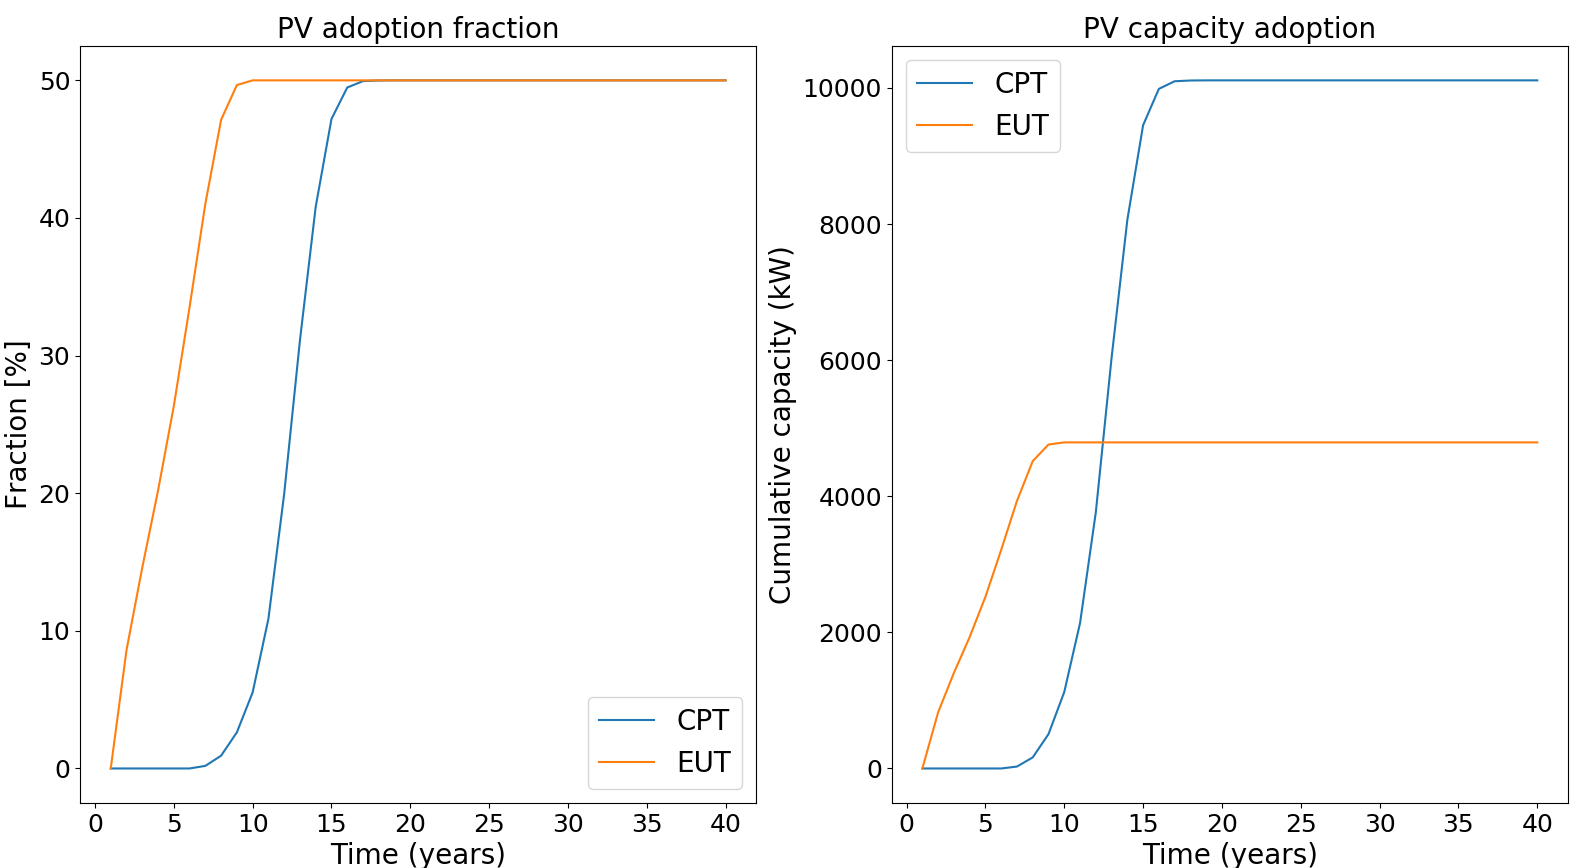
\includegraphics[width=12cm]{EUTCompar/PV.png}
\caption{PV adoption comparison}
\label{Figure:PVcompar}
\end{figure}
%\newline \newline
\noindent
Whereas the PV adoption shows an S-shaped adoption curve, this does not apply to the battery technology. The battery adoption results for the EUT remain equal to zero, as can be seen in Figure \ref{Figure:bateut}. A comparison of this adoption data with the data of the CPT can be found in \ref{Figure:batcompar}:
%\newline
%\begin{figure}[h!]
%\centering
%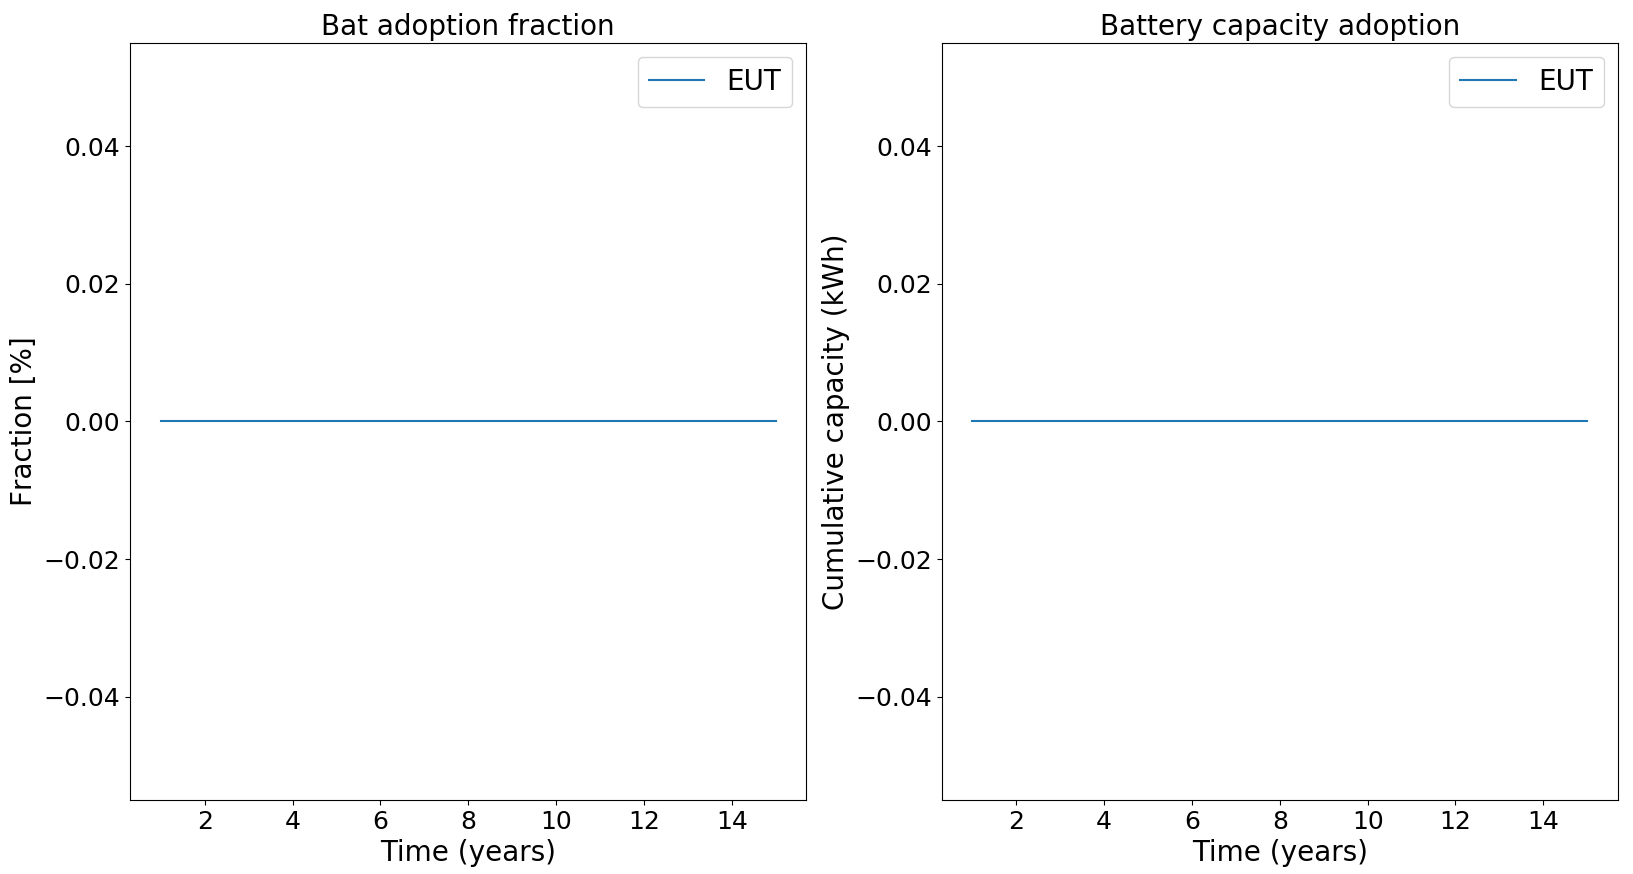
\includegraphics[width=12cm]{EUTCompar/BatEUT.png}
%\caption{Battery adoption under EUT}
%\label{Figure:bateut}
%\end{figure}
%\noindent
%\newline
\begin{figure}[h!]
\centering
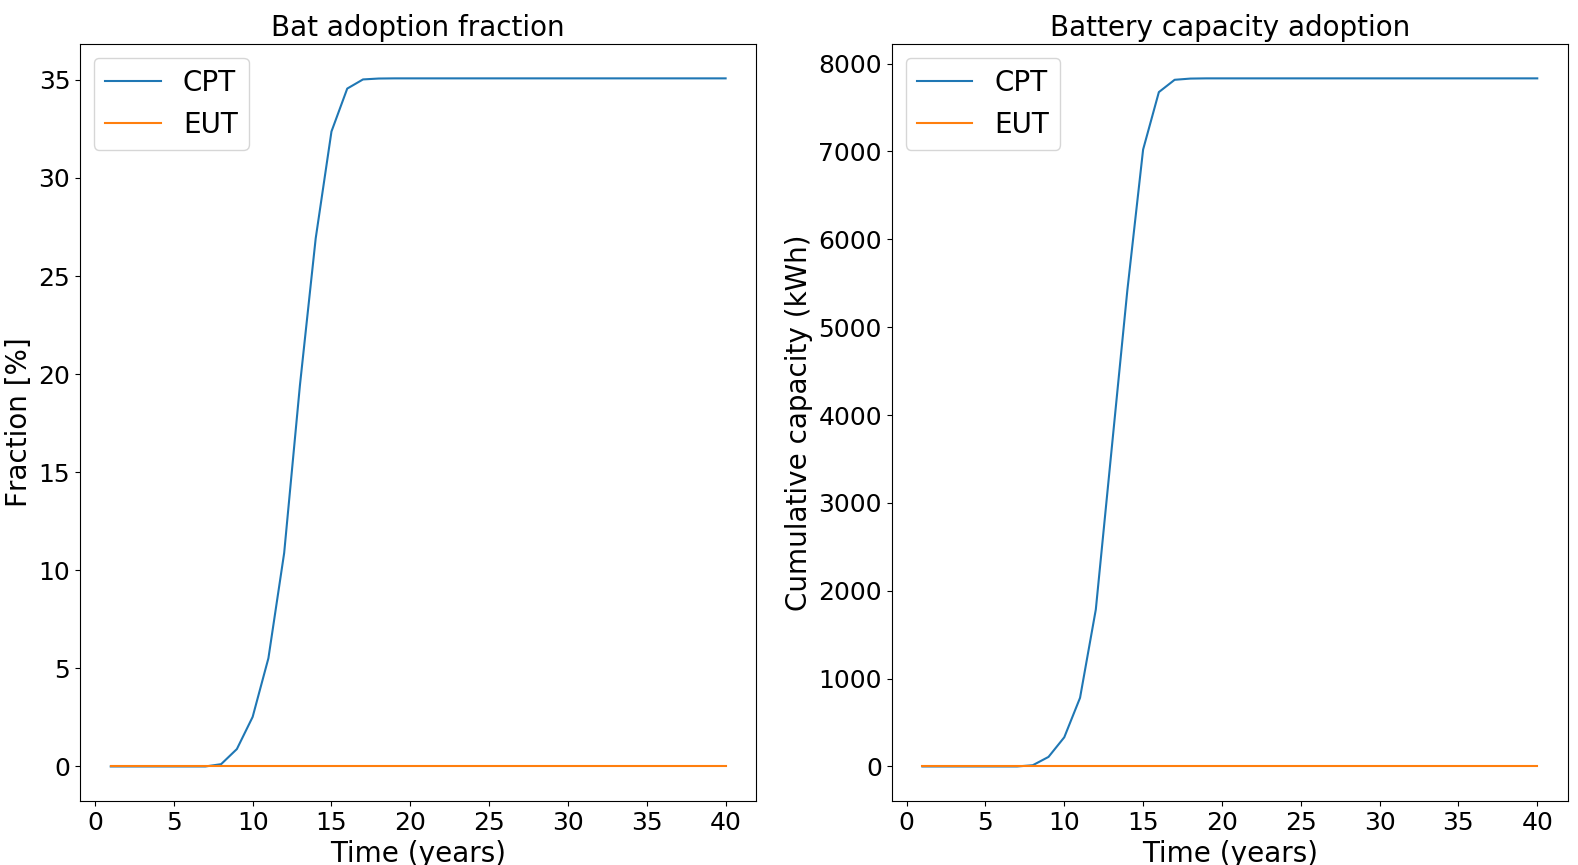
\includegraphics[width=12cm]{EUTCompar/Bat.png}
\caption{Battery adoption comparison}
\label{Figure:batcompar}
\end{figure}
%\newline 
\noindent
The main reason for this lack of battery adoption is because the adoption will happen according to the normalised payback period. The higher the payback period, the lower the normalised utility is, according to Equation \ref{EUTnorms}. The preferred options, therefore, will be those with the lowest overall payback. As can be seen from Figure \ref{Figure:payback}, the 1.5 \textit{kW} and 2.5 \textit{kW} configurations without any batteries have the lowest payback period. These technologies will, therefore, have the highest economic utility and will be the preferred options for the households. As a result, no batteries will be adopted under the EUT simulation. In fact, the EUT model would require battery subsidies that exceed the capital cost of the battery technology to encourage any adoption of battery configurations.
\newline 
\begin{figure}[h!]
\centering
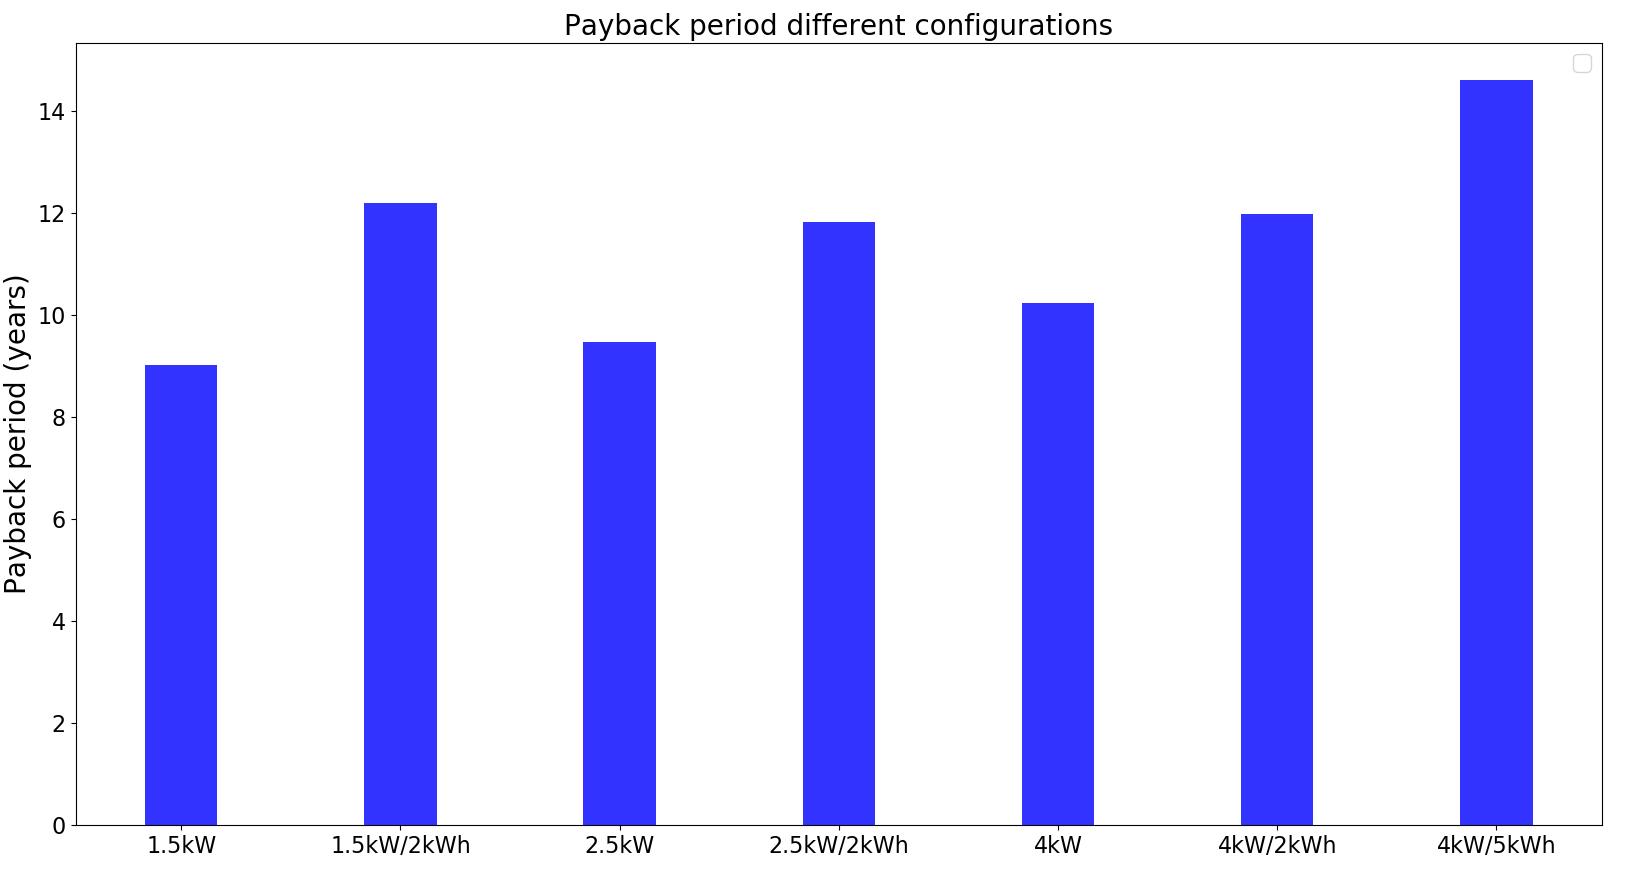
\includegraphics[width=12cm]{EUTCompar/Payback.png}
\caption{Initial payback periods}
\label{Figure:payback}
\end{figure}
\newline \newline \noindent
This shows how the EUT is less refined and complex as a decision-making theory, since there is a subtle bias in the selection. Due to the reference level incorporated in the CPT, different households have different utility patterns which will cause the adoption to be more diverse: laggards can have a completely different economic view on a certain configuration than innovators do. The added level of complexity that CPT modeling requires by incorporating loss aversion and reference levels, controversial though these concepts may be, seem to show their added value in the results, since results using this theory are less lopsided than the EUT results. 
\newline \newline \noindent
When looking at how the overall configuration distribution compares for both decision making theories, there is a very clear difference in the results, as can be seen in Figure \ref{Figure:configeut}. This data reconfirms the aforementioned bias of EUT towards small PV configurations without batteries: the overwhelming majority of configurations adopted under EUT is the 1.5\textit{kW} PV installation, with a small minority in 2.5\textit{kW} configurations adopted. When using the CPT, the adoption is more granular between the different technologies, both standalone PVs and PV-battery systems, with 4\textit{kW}/2\textit{kWh} and 4\textit{kW}/5\textit{kWh} being the most popular.
\begin{figure}[h!]
\centering
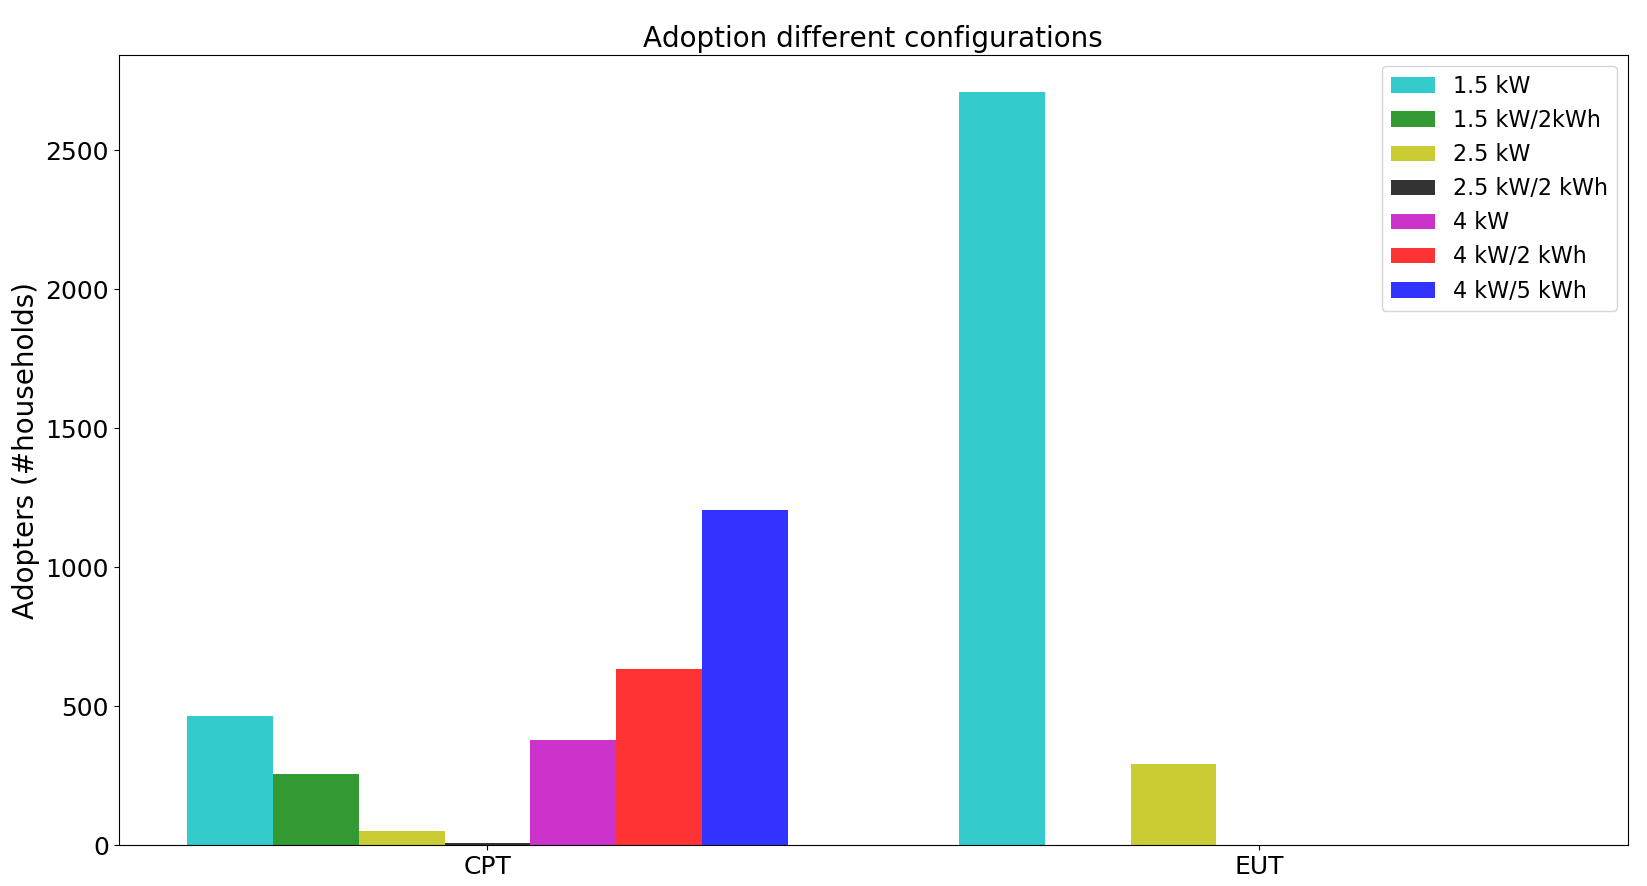
\includegraphics[width=12cm]{EUTCompar/Config.png}
\caption{Configurations comparison}
\label{Figure:configeut}
\end{figure}
\noindent
In parallel with the adoption for the different decision making theories, the network charge will evolve to very rapidly for the EUT and at a slower but more steady rate for the CPT.
\begin{figure}[h!]
\centering
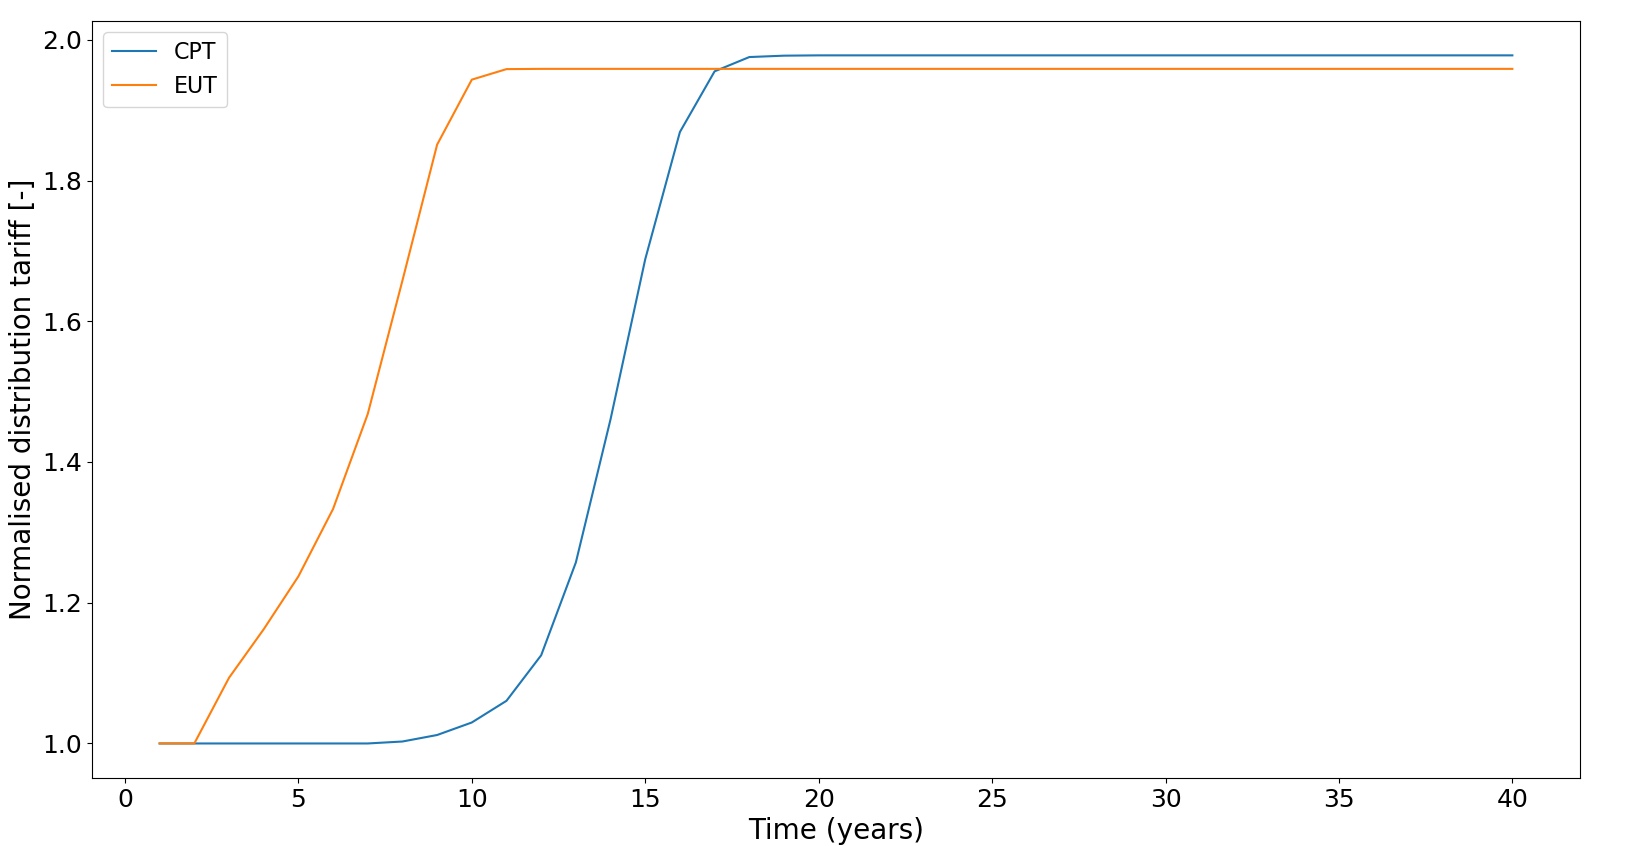
\includegraphics[width=10cm]{EUTCompar/Dist.png}
\caption{Distribution cost comparison}
\label{Figure:distcompar}
\end{figure}
\subsection{Annual capacity offtake tariff}
The PV adoption for the annual capacity offtake tariff can be found in Figure \ref{Figure:PVeutcap}. Here, the adoption trend of the PV technology can be seen, which starts quickly in the beginning (innovators and early adopters), followed by a period of rapid adoption, only to end with a period of saturated adoption (when the laggards will adopt). The adoption does, therefore, once again follow and S-shaped evolution, except for the start of the adoption. 
\newline
\begin{figure}[h!]
\centering
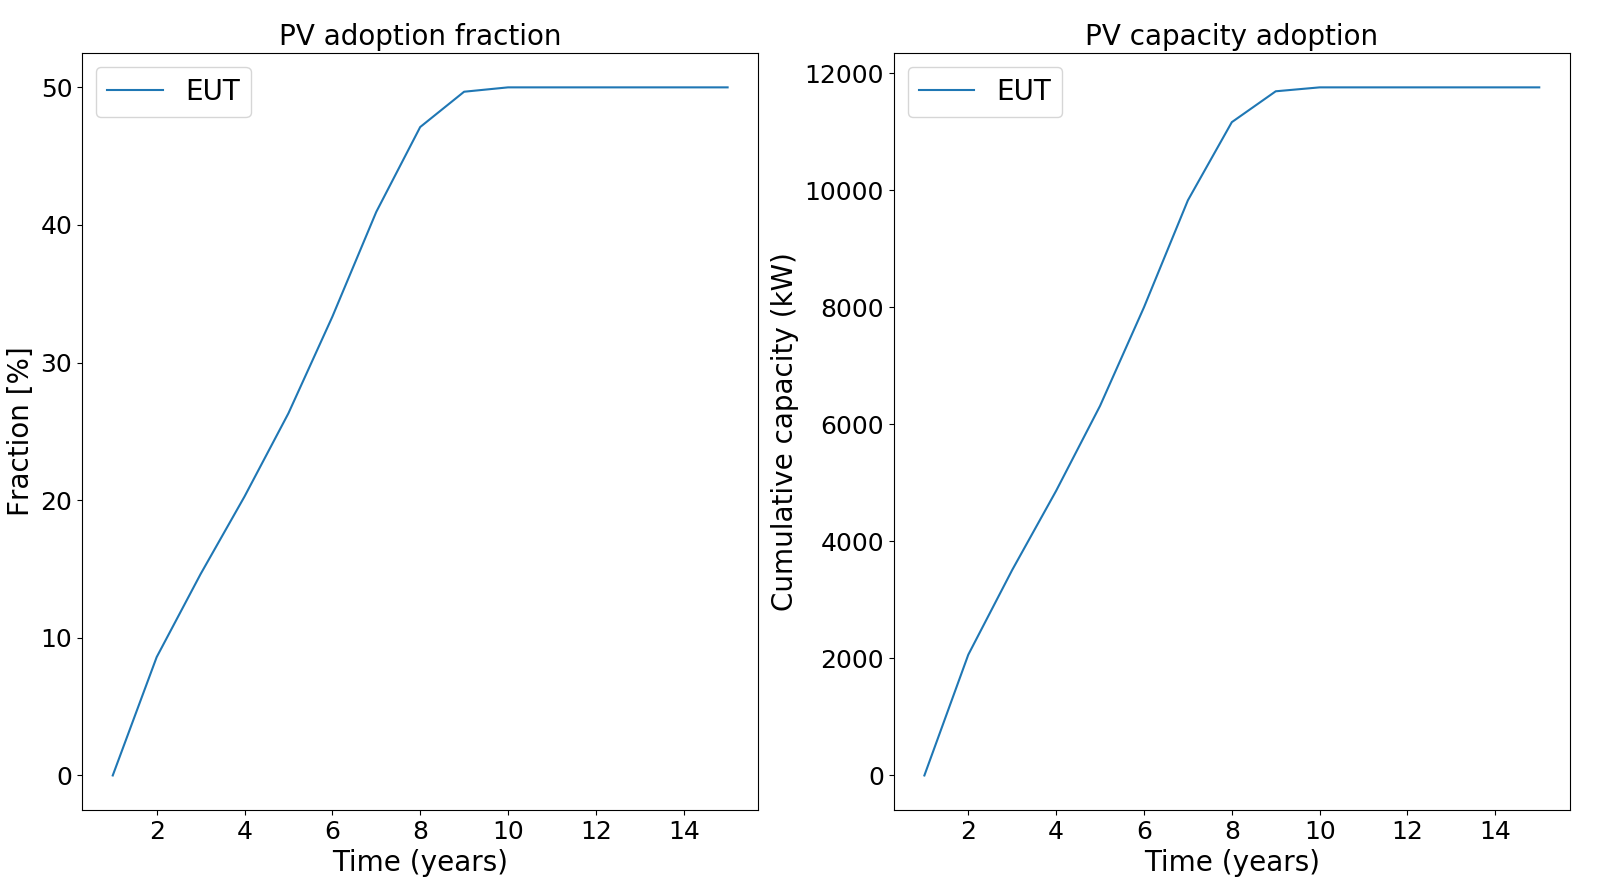
\includegraphics[width=14cm]{EUTCompar/PVEUTcap.png}
\caption{PV adoption under EUT}
\label{Figure:PVeutcap}
\end{figure}
\noindent 
When comparing the results of the EUT with those of the CPT, as can be seen in Figure \ref{Figure:PVcomparcap}, there is a big difference in the adoption trend. As was the case for the net volumetric distribution tariff, the adoption in the EUT case will happen both earlier in the simulation and more quickly, whereas the adoption in the case of the CPT will both happen in a later stage and happen at a slower but steadier rate. Despite both decision making theories providing results that correspond to the logic behind Rogers' adoption process of innovation diffusion, the scale of this adoption process is rather different. Both simulations start with lower adoption rates, followed by higher adoption rates only to saturate toward the final adoption rate. In the case of the EUT, however, this adoption process happens very sudden, whereas the process is much more gradual for the CPT simulation. As was the case with the net volumetric distribution tariff, these results both confirm the validity of the separate decision making theories with regards to the adoption process, but the vast difference in the overall adoption process gives rise to one major question, which is why the adoption process is so different for the two decision making theories.
 \newline \noindent
 \begin{figure}[h!]
\centering
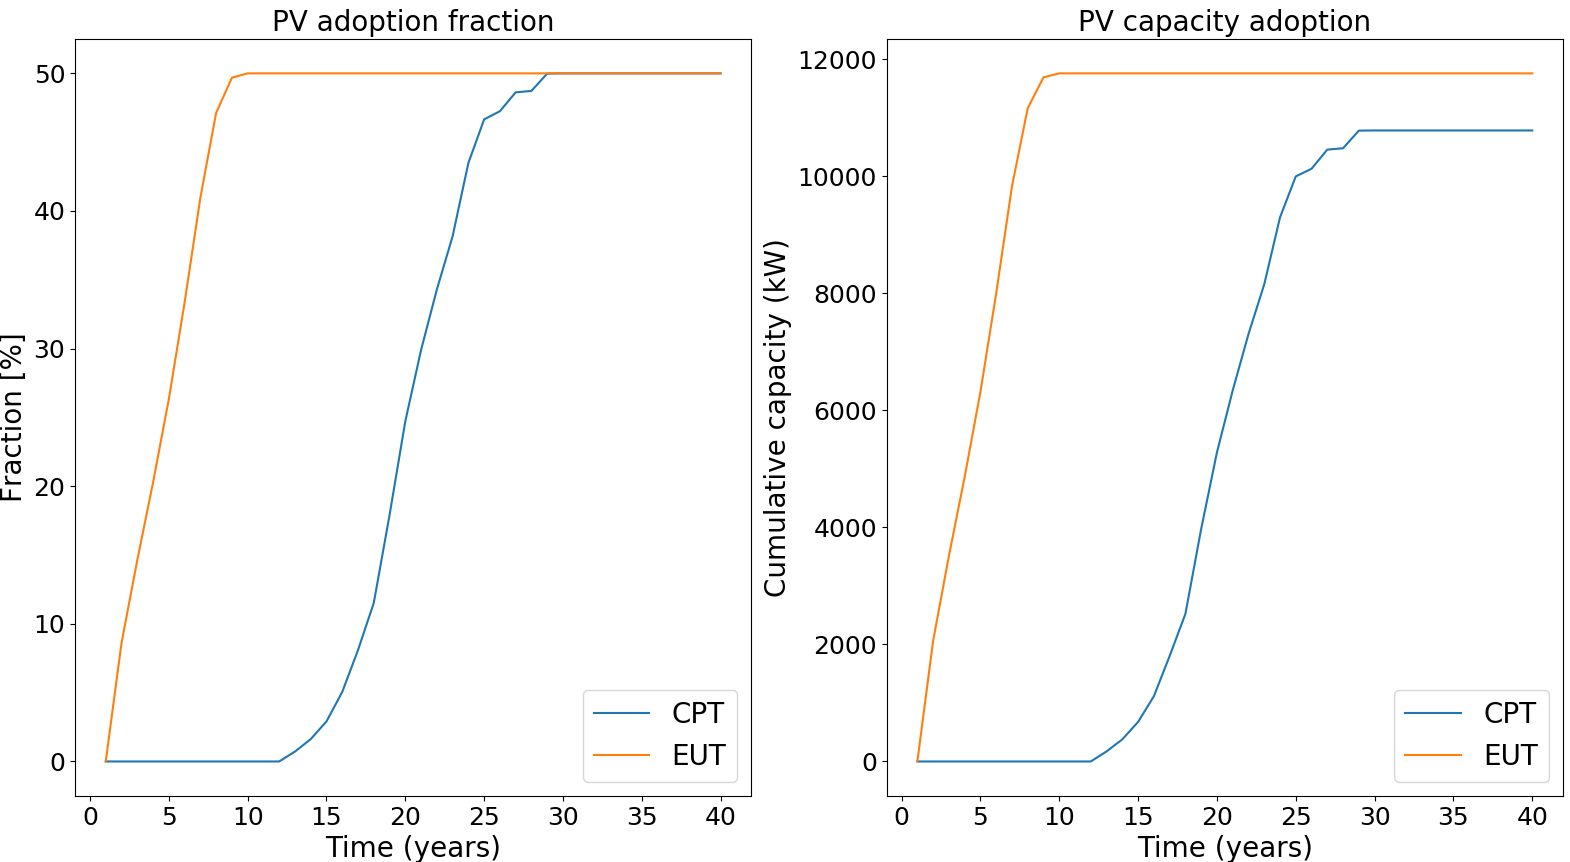
\includegraphics[width=14cm]{EUTCompar/Pvcap.png}
\caption{PV adoption comparison}
\label{Figure:PVcomparcap}
\end{figure}
\newline \newline \noindent
One of the main reasons, for this difference in adoption, as was the case with the net volumetric distribution tariff, is the incorporation of loss aversion into the simulation by using CPT. According to Equation \ref{EUTnorms}, the normalised economic utility of the configurations cannot be negative. This implies that however large the payback period of the different configurations, there will still be some level of positive economic utility to the investment options under consideration. This will implicitly make the household more prone to adopt one of the DERs available. When using the CPT, on the other hand, there will be a clear distinction between configurations that the household will consider as being economically attractive and those that he considers economically disadvantageous. Given the fact that the loss aversion will make the households "overweight" the negative prospects of those disadvantageous configurations by a factor of 2.25, households will be loss prone to adopt one of the DERs at hand. Since the households will initially be a bit "frightened" by the negative prospects of the DERs, adoption will only happen in a later stage, when cost reduction effects have manifested themselves sufficiently to make the overall prospects more positive. 
\newline \newline \noindent
The battery adoption for the capacity tariff under EUT can be found in Figure \ref{Figure:bateutcap}.
\newline
\begin{figure}[h!]
\centering
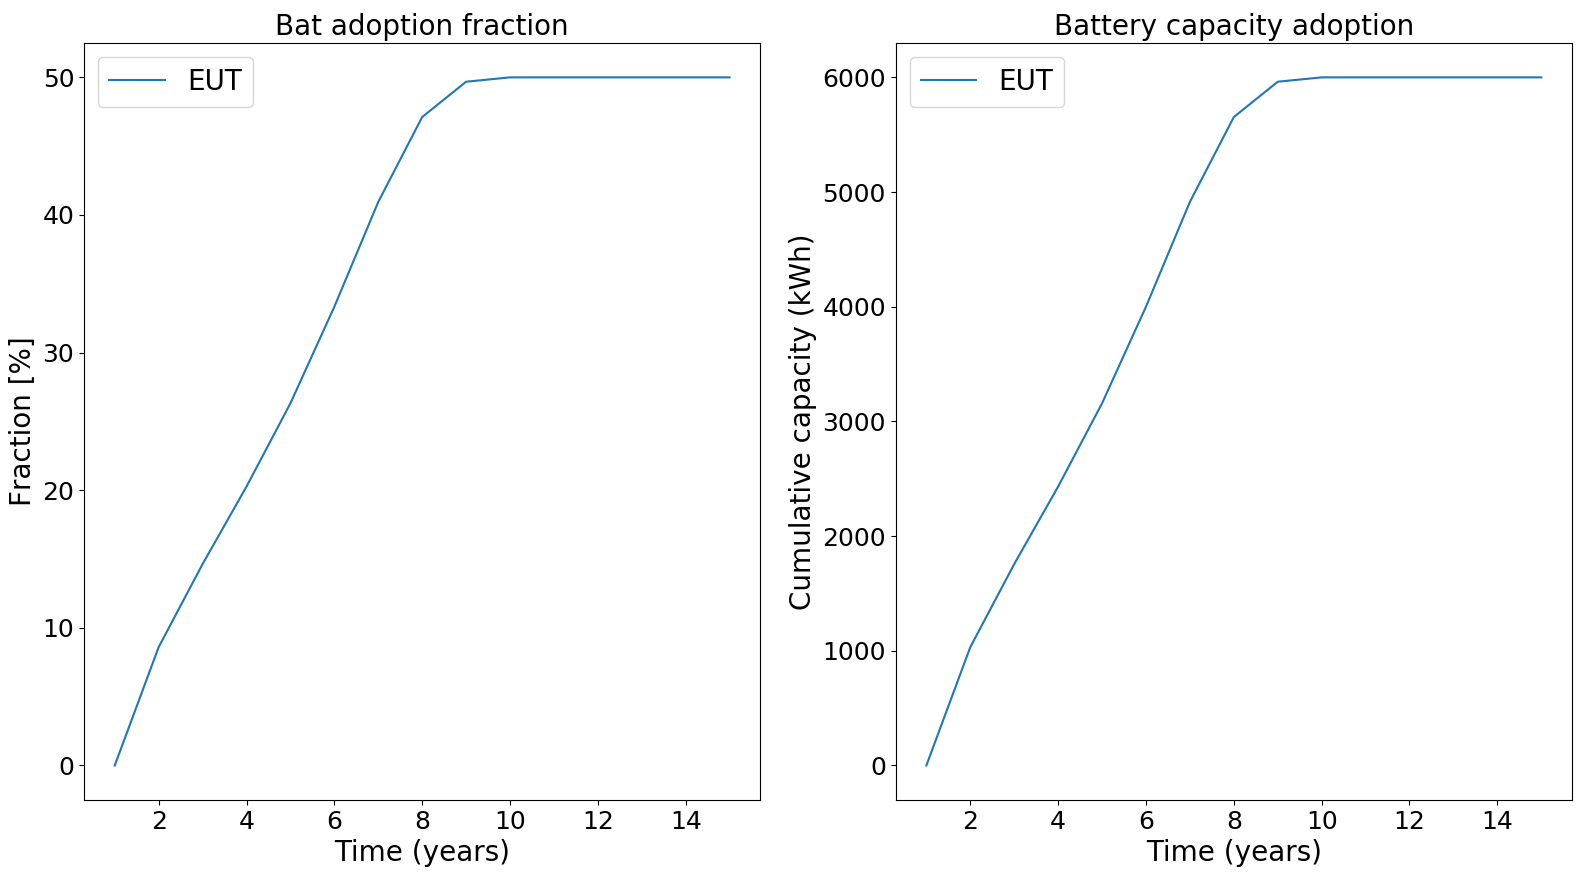
\includegraphics[width=14cm]{EUTCompar/BatEUTCap}
\caption{Battery adoption under EUT}
\label{Figure:bateutcap}
\end{figure}
\newline
\noindent 
Contrary to the net volumetric distribution tariff case, the EUT simulation under the annual capacity offtake tariff will result in battery adoption. This adoption process also saturates to a level of full adoption. The adoption process will also follow the known S-curved adoption process, except for the start of the adoption where the adoption rate is higher. When comparing this data to the CPT case, as can be seen in Figure \ref{Figure:batcomparcap}, the adoption data once again shows a big difference for the two different decision making theories. As was the case for PV adoption, the battery adoption using the EUT happens at an earlier stage and at quicker rates.
\begin{figure}[h!]
\centering
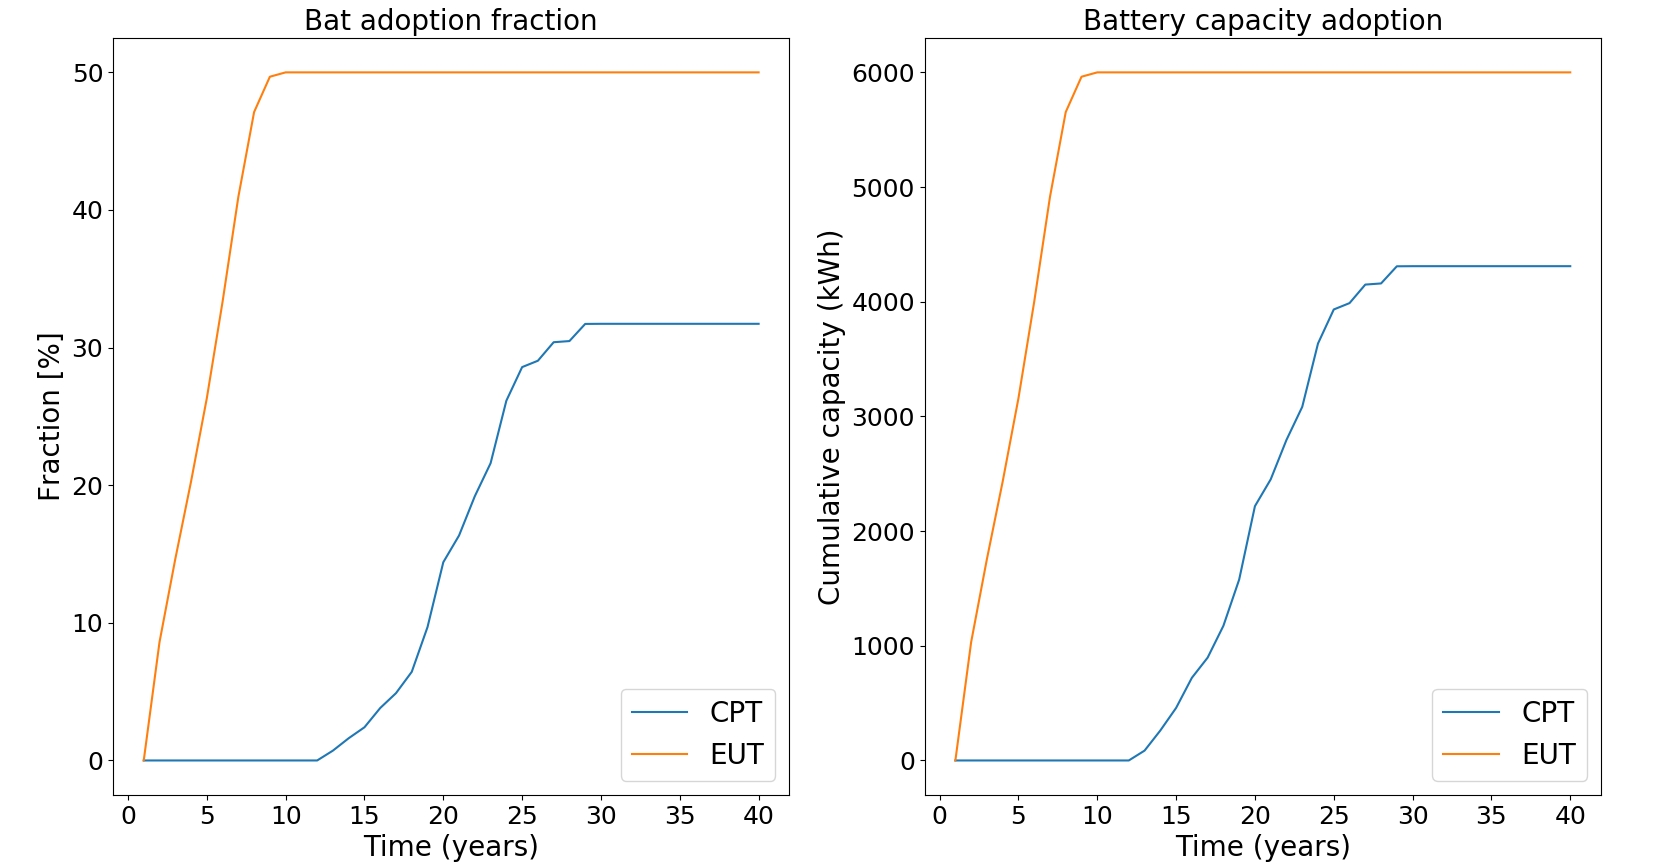
\includegraphics[width=14cm]{EUTCompar/BatCap.png}
\caption{Battery adoption comparison}
\label{Figure:batcomparcap}
\end{figure}
\noindent 
Once again, this is due to the popularity of certain configurations. Figure \ref{Figure:paycap} show how the 2.5\textit{kW}/2\textit{kWh} and 4\textit{kW}/2\textit{kWh} configuration have the lowest payback period in the EUT simulation for the annual capacity offtake tariff. This is due a combined effect of the low peak capacity (see Section \ref{distanal}) and the initial investment cost. Although the peak capacity of the 4\textit{kW}/5\textit{kWh} configuration is the lowest of all the options (see Figure \ref{Figure:peakdem}), the savings due to this lower peak capacity are not sufficient to compensate for the higher investment cost. 
\newline 
\begin{figure}[h!]
\centering
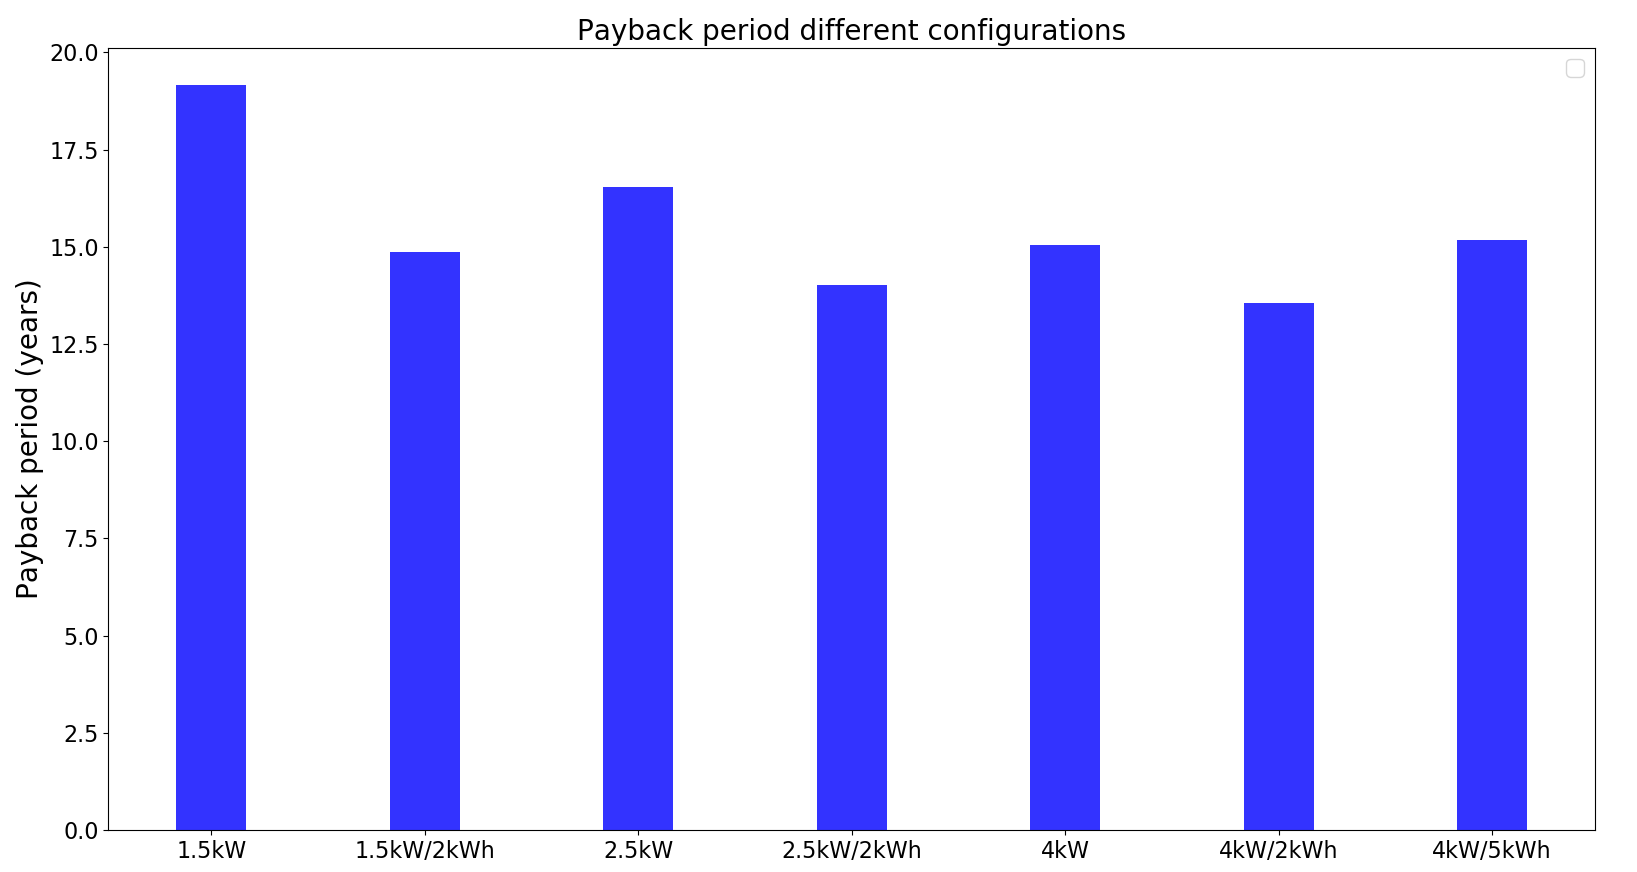
\includegraphics[width=10cm]{EUTCompar/PayCap.png}
\caption{Initial payback periods}
\label{Figure:paycap}
\end{figure}
 \newline \newline \noindent 
 This combined effect of savings and investment cost will make the 4\textit{kW}/2\textit{kWh} configuration the most popular, as can be seen in Figure \ref{Figure:comparcap}. Whereas the CPT simulation shows a distribution of the different configurations adopted, the EUT simulations shows a very clear adoption bias towards the two aforementioned configuration. 
 \begin{figure}[h!]
\centering
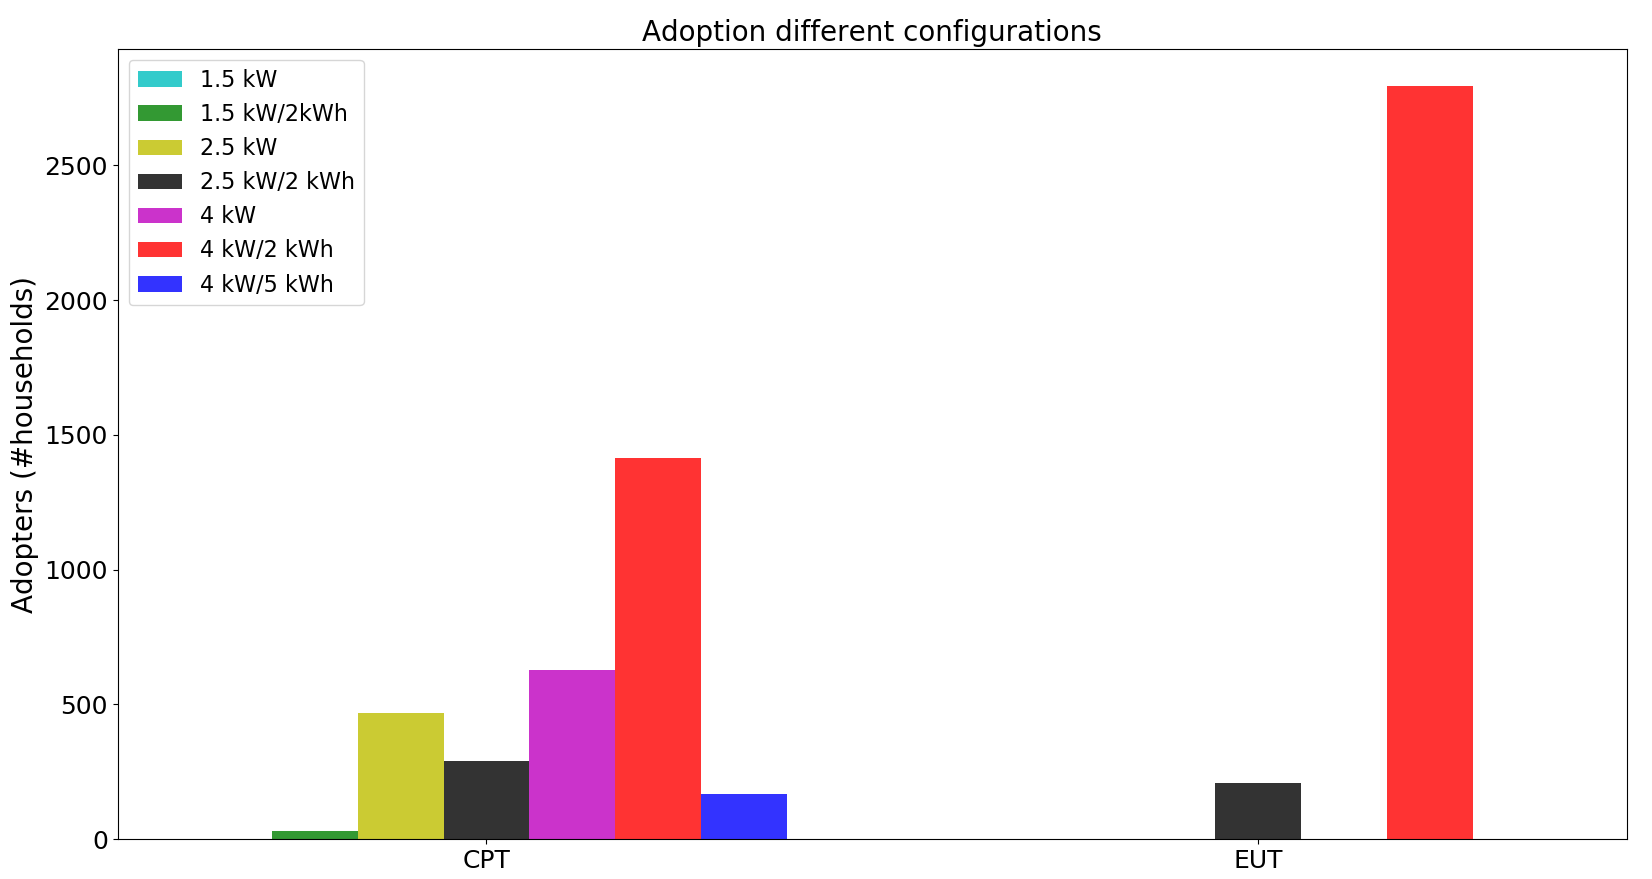
\includegraphics[width=10cm]{EUTCompar/ConfigCap.png}
\caption{Configurations comparison}
\label{Figure:comparcap}
\end{figure}
\newline \newline \noindent 
 As a final note, the capacity offtake tariff evolution can be found in Figure \ref{Figure:captar}.  Given the further stage of DERs adoption in the case of EUT, the capacity tariff will decrease further, due to reasons explained in Section \ref{distanal}. 
\begin{figure}[h!]
\centering
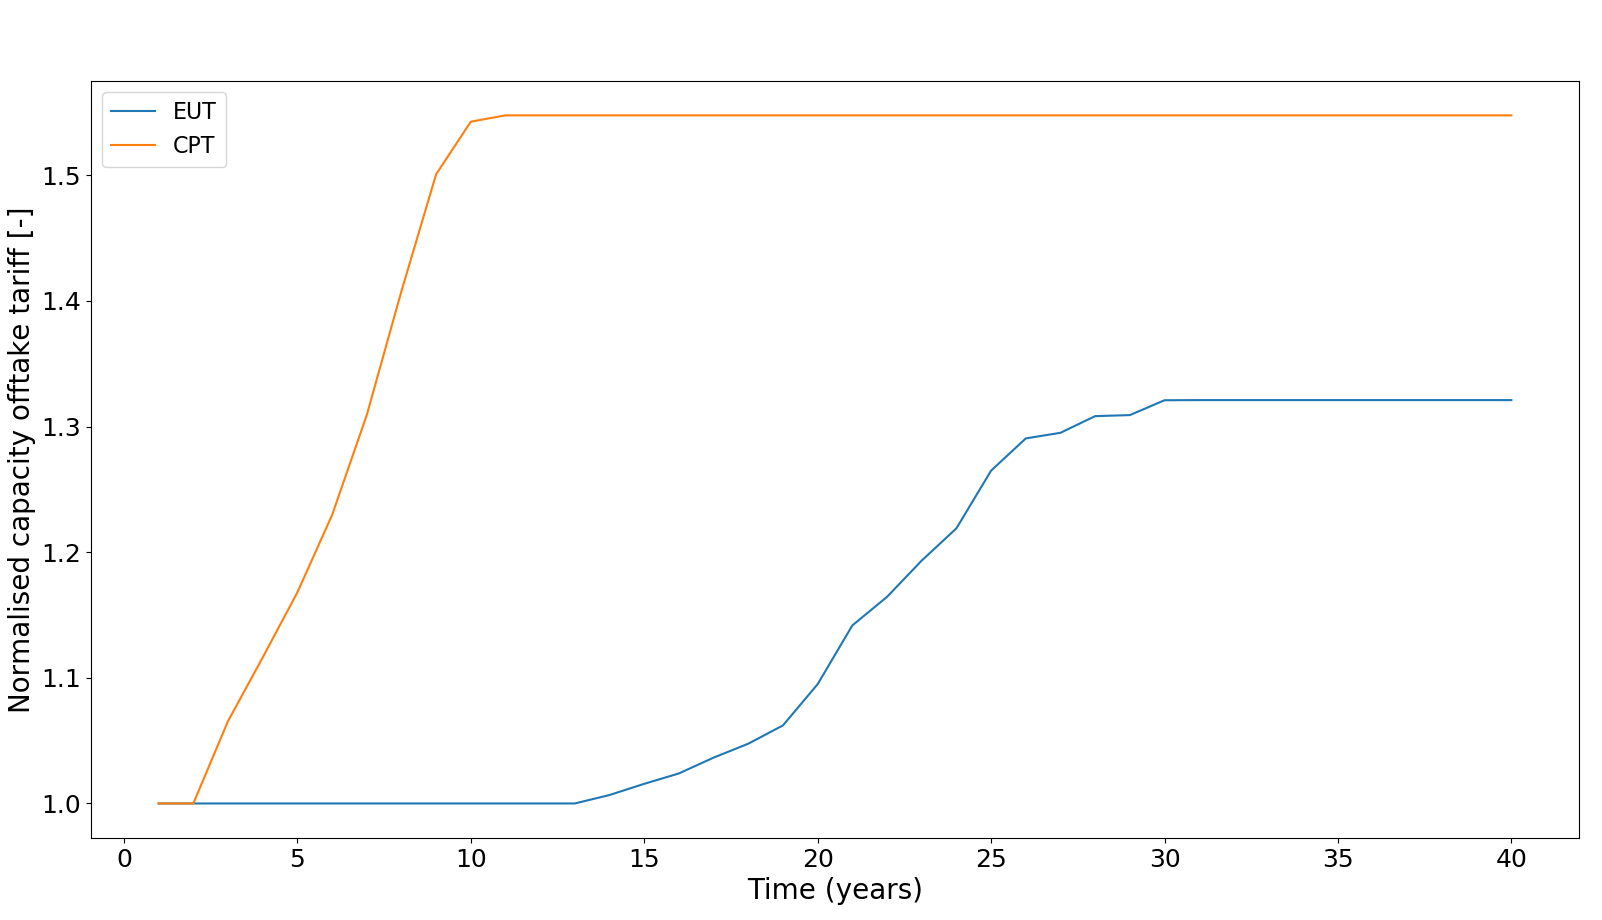
\includegraphics[width=10cm]{EUTCompar/CapTar.png}
\caption{Capacity tariff evolution}
\label{Figure:captar}
\end{figure}
\subsection{Preliminary analysis \& Conclusion}
With the previously discussed data in mind, EUT does seem to present much cruder results than the CPT. The added complexity of accounting for loss aversion and the reference level of each decision maker (by comparing the expected payback period with the actual payback period of configurations) clearly adds an additional level of complexity to the results. Given the more gradual adoption of technologies due to the loss aversion and the more granular adoption of different technologies by accounting for the reference level of each household, this added level of complexity does appear to add relevance to the results. 
\newline \newline \noindent
Considering the fact that only two utility attributes (economic and social utility) were used in this simulation, whereas other works use three or more utility attributes \footnote{Zhao et al. \cite{ABMPV} consider payback periods, household income, advertisement and neighborhood effects as utility attributes in their model whereas Palmer at al. \cite{ItalyAdoption} consider the payback period, environmental benefits, household income and communication effects as attributes in their model}, elaborating on these utility attributes using CPT could generate results of increased quality and resemblance to real-life adoption data. 
\newline \newline \noindent
Despite the fact that many items still need addressing in this setting, like a further diversification of the economic factors in the model, the constant weighting coefficients in the utility and the extent of the utility attributes themselves, the presented results have made a strong case for CPT as a decision making theory in the simulation of investments in DERs in consumer-centric energy systems.
\section{Discussion \& Future work} \label{future}
In this section, the results of the model were discussed in order to address the research question and the complementary sub-questions. This discussion was separated according to these research questions. The first research question related to the evaluation of different policies with regards to the DER adoption and utility death spiral. The main takeaways here are:
\begin{itemize}
\item The net billing policy can serve as an efficient way to encourage rapid adoption of small-scale DERs. These installations will predominantly serve the inflexible demand of the households and inject a limited amount of electricity into the grid.
\item The net metering policy and additional battery subsidies can serve as a way to encourage large cumulative adoption capacity of DERs installations. These policies will, however, cause larger amounts of grid injection. Their efficiency is, therefore, questionable.
\item The net volumetric distribution tariff will encourage larger and quicker adoption of PV and batteries due to larger savings. In parallel, the utility death spiral (i.e. tariff modification by the DSO) will manifest itself more clearly. The capacity offtake tariff, on the other hand, can partially mitigate the effects on this utility death spiral, indicating that this network charge is preferable in the future grid, where widespread DER adoption and the subsequent utility death spiral are extremely likely prospects. 
\end{itemize}
The second Research Question, which is a sub-question to the main Research Question, relates to the sensitivity of certain parameters embedded in the model. 
\begin{itemize}
\item The selected value for the loss aversion coefficient ($\lambda = 1.5$)  can provide a consistent set of results and suggest that future research into adequate values of this parameter can add valuable insights. 
\item The lower the residual load the DSO can rely on, the more the utility death spiral will manifest itself. In the future grid, where DER adoption becomes more pervasive, this effect will become increasingly present and is a threat that must be anticipated. The capacity tariff is a means to mitigate this utility death spiral effect.
\item Battery subsidies can help encouraging the adoption of residential batteries combined with PV, but the main effect of these subsidies is the increased adoption of the largest configurations available, causing large-scale grid injection. Given the amount of government resources these subsidy programs require, this subsidy may not be necessary if the battery technology sufficiently expands and scales in cost in the near future, since the battery cost reduction also is an important driver in the battery adoption process. 
\end{itemize}
The third Research Question, which also is a sub-question to the main Research Question, relates to the comparison of the model results with the EUT.
\begin{itemize}
\item  CPT as a decision making theory to simulate the adoption of DER in consumer-centric energy systems can complement the results provided by the EUT.
\item The results of EUT compared to the CPT are cruder and less refined, since the adoption does not follow the same adoption trend and tends to focus the adoption or one of two configurations. 
\item Despite uncertainty concerning some of the parameters in CPT, like the loss aversion, risk aversion and reference levels, this theory can capture more complex behavior of decision makers, like being able to describe a more diverse configuration adoption.
\end{itemize}
\newline \newline \noindent
Despite these insights, further work still needs to be done in this field. First and foremost, since this Thesis attempted to provide qualitative insights into this novel approach to the simulation of DER adoption by using CPT, a case test must be performed to relate this research to the real world. This must be complemented by field experiments where energy prosumers are the targets to be able to measure an accurate value of the loss aversion, risk aversion and reference levels. In addition, a number of items need further elaboration:
\begin{itemize}
\item Since the utility calculation only considers economic and social utility but many more factor have an effect on the adoption such as advertisements, household profiles etc, the utility attributes must be extended beyond the two considered in this Thesis.
\item Some implicit assumption made concerning the behavior of the households, like the absence of the rebound effect and the indifference of the residual households towards the increase in distribution tariffs, must be elaborated upon. 
\item Since the diversification of the household was limited to the financial wealth of the household, this diversification must be elaborated to social, geographical and cultural factors influencing the nature of the households and his position towards DERs adoption under uncertainty.
\item The assumption of constant weighting coefficients and the constant adoption nature of the different households must be elaborated to a model where these parameters also become endogenous to the model and change over time: initially the economic weighting coefficient should be larger, but as the adoption proceeds over time, the social weighting coefficient should be larger.
\item Whereas this Thesis considers the different policies separately, different combinations the presented policies should be examined to find an optimal structure that can combine the positive effects of the respective policies while minimizing the negative effects of these programs. An example could be a policy that combines the quick adoption rates of the net billing policy with the limited utility death spiral effects of the annual capacity offtake policy. 
\item In addition to the parameters tested in the model, the time preference behavior of the households, which is captured through the discount factor, must be included in the model analysis. In doing so, this must be related to the loss aversion of the households to test different configurations of this behavior. 
\end{itemize}
Despite these items that need further work in this field, the results in this chapter have made a strong case for further research into CPT in an ABM for the simulation of DER adoption in a consumer-centric energy system, which was assumed to be a CAS. 
